\documentclass{tufte-handout} 
\usepackage{amsmath,stmaryrd,amssymb,amsthm,url,booktabs,hyperref,enumerate}
\usepackage{color}
\usepackage{tikz}
\usetikzlibrary{decorations.markings}
\usepackage{stackrel}

% \usepackage{enumitem} \setlist[itemize]{noitemsep, topsep=0pt}

\makeatletter
% Paragraph indentation and separation for normal text
\renewcommand{\@tufte@reset@par}{% 
  \setlength{\RaggedRightParindent}{0pc}% 1.0pc 
  \setlength{\JustifyingParindent}{0pc}% 1.0pc 
  \setlength{\parindent}{0pc}% 1pc 
  \setlength{\parskip}{0pt}%
}
\@tufte@reset@par

\makeatother


\ifpdf 
	\usepackage[all,pdf,cmtip]{xy} %% NB this MUST be loaded last.
\else
	\input xy 
	\xyoption{all} 
	\xyoption{2cell} 
	\xyoption{v2}
\fi 
\CompileMatrices

\parskip = 10pt

\def\into {\hookrightarrow} 
\def\cE {\mathcal{E}} 
\def\cC {\mathcal{C}} 
\def\cR {\mathcal{R}} 
\def\cD {\mathcal{D}} 
\def\cP {\mathcal{P}} 
\def\cT {\mathcal{T}} 
\def\cN {\mathcal{N}}

\def\op {\mathrm{op}}
\def\pt {\mathrm{pt}}

\def\Set {\mathbf{Set}}
\def\Top {\mathbf{Top}}
\def\Ho {\mathbf{hTop}}
\def\slpcTop {\mathbf{slpcTop}}
\def\Cov {\mathbf{Cov}}
\def\Grp {\mathbf{Grp}}
\def\Gpd {\mathbf{Gpd}}
\def\Mod {\mathbf{Mod}}
\def\Ab {\mathbf{Ab}}
\def\Fin {\mathbf{Fin}}
\def\Vect {\mathbf{Vect}}


\def\RR{\mathbb{R}} 
\def\NN{\mathbb{N}}
\def\ZZ{\mathbb{Z}}
\def\QQ{\mathbb{Q}}
\def\CC{\mathbb{C}}
\def\BB{\mathbb{B}}

\newcommand{\lecturenum}[1]{\marginnote{\color{red}Lecture #1}}

\DeclareMathOperator{\disc}{disc}
\DeclareMathOperator{\codisc}{codisc}
\DeclareMathOperator*{\colim}{colim} 
\DeclareMathOperator{\Sh}{Sh} 
\DeclareMathOperator{\id}{id} 
\DeclareMathOperator{\Sub}{Sub} 
\DeclareMathOperator{\Aut}{Aut} 
\DeclareMathOperator{\Cont}{Cont}
\DeclareMathOperator{\im}{im}
\DeclareMathOperator{\pr}{pr}
\DeclareMathOperator{\ev}{ev}
\DeclareMathOperator{\Lift}{Lift}
\DeclareMathOperator{\Ad}{Ad}

\theoremstyle{definition} 
\newtheorem{prop}{Proposition} 
\newtheorem{lemma}{Lemma} 
\newtheorem{definition}{Definition} 
\newtheorem{example}{Example} 
\newtheorem{ex}{Exercise}
\newtheorem{construction}{Construction}
% \newtheorem{exercise}{Exercise} 
\newtheorem{theorem}{Theorem} 
\newtheorem{corollary}{Corollary} 
\newtheorem{q}{Question} 
\newtheorem*{conj}{Conjecture} 
\newtheorem*{rem}{Remark} 
\newtheorem*{fact}{Fact}

\newenvironment{psmallmatrix}
  {\left(\begin{smallmatrix}}
  {\end{smallmatrix}\right)}

\title{Algebraic Topology\thanks{This document is released under a CC-By license: 
\href{https://creativecommons.org/licenses/by/4.0/}{\texttt{creativecommons.org/licenses/by/4.0/}}.}
}
\author[D.M.~Roberts]{David Michael Roberts} 
\date{2019} 

\begin{document} 

\maketitle

\lecturenum{1} \section{What is it?}

Algebraic topology is the study of maps 
\[
	\{\text{Spaces}\} \longrightarrow \{\text{Algebraic objects}\},
\] 
%
or rather, `well-behaved' such maps. They should also send continuous functions between spaces to 
algebraic maps, respecting composition (so: \emph{functors}); they should send spaces built 
out of simpler spaces to algebraic objects built out of simpler components, in a compatible way, 
etc.

Here, `Spaces' roughly means topological spaces up to deformation (usually homotopy, but 
not always). Such equivalence classes are called \emph{homotopy types}. `Algebraic 
objects' means (abelian) groups, rings, modules, or even chain complexes of these 
\marginnote{a chain complex is a certain sequence of maps $\cdots \to V_0 \to V_1 \to 
V_2 \to \cdots$}.

\begin{example} 
	How can we tell if the sphere $S^2$ and the torus $S^1\times S^1$ can or 
	cannot be deformed into each other? How would you prove it cannot be done? 
\end{example}

\begin{example} 
	For a positive example, we \emph{can} squash $\RR^3 \setminus \{0\} \to S^2 \into 
	\RR^3 \setminus \{0\} $, sending $x\mapsto \frac{x}{|x|}$. This map continuously 
	deforms to the identity map. So dimension not necessarily preserved.
\end{example}

\begin{example} 
	Can we have $S^1 \sim S^2$? 
\end{example} 

\noindent We first need to understand how spaces are built

\section{Topological spaces}

Recall\ldots\marginnote{From Topology and Analysis III}

\begin{definition} 
	A \emph{topology} on a set $X$ is a collection $\cT$ of subsets of $X$ 
	such that 
	\begin{enumerate} 
	
		\item $\emptyset,X\in\cT$ 
		
		\item If $U,V\in \cT$ then $U\cap V\in \cT$ 

		\item If $\{U_\alpha\}_{\alpha\in I}$ is an arbitrary family of sets in $\cT$, then $\bigcup_{\alpha\in I} U_\alpha \in \cT$\marginnote{$I$ here is an indexing set}

	\end{enumerate}
 
	If $U\in \cT$ we say $U$ is \emph{open}. A \emph{topological space} is a set $X$ 
	eqipped with a topology $\cT$.
\end{definition}

\begin{example} 
	Take the set of real numbers, the \emph{Euclidean (`usual') topology} is 
	defined by saying a set is open iff it is a union of open intervals $(a,b)$ (including the 
	union of no sets ie $\emptyset$).\\ 
	The \emph{discrete topology} on a set $X$ is defined by 
	taking every $\cT$ to consist of all subsets. The \emph{indiscrete topology} is defined by 
	taking $\cT$ to consist of just $\emptyset$ and $X$. 
\end{example}

This definition is concise, but not always the best way to define a topology. We will also 
use \emph{neighbourhoods}

\begin{definition} 
	A set $N\subseteq X$ is a \emph{neighbourhood}\marginnote{`nhd' is a good 
	abbreviation} (in a given topology $\cT$) of a point $x\in X$ if there is an open 
	set $U\subseteq N$ with $x\in U$.
\end{definition}


\begin{example} 
	Take $\RR$ with the Euclidean topology. $(-1,1)$, $[-1,1]$, $[-1,1)$ are all 
	neighbourhoods of every $-1<x<1$, but $[0,1)$ is not a neighbourhood of $0$. More 
	complicated: $[0,1] \cup \{2\}\cup [5,6]$ is a nhd of all $0<x<1$ and $5<x<6$.
\end{example}

\begin{example} 	
	Consider a metric space $(X,d)$. The \emph{metric topology} is defined by saying a 
	subset $U\subseteq X$ is open iff for every $x\in U$ there is some $\varepsilon_x > 
	0$ with the open ball $B(x,\varepsilon_x) \subseteq U$. Open balls around $x$ are 
	neighbouhoods of $x$, as are closed balls.
\end{example}

Here is a more concrete approach that allows concise definitions of topologies:

\begin{definition} 
	A \emph{neighbourhood base} $\cN$ on a set $X$ is a family 
	$\{\cN(x)\}_{x\in X}$ where each $\cN(x)$ is a nonempty collection of subsets of $X$, 
	satisfying the following, for all $x\in X$: 

	\begin{enumerate} 

	\item For all $N\in \cN(x)$, $x\in N$;
 
	\item For all $N_1,N_2 \in \cN(x)$, there is some $N\in \cN(x)$ with $N\subseteq N_1 
	\cap N_2$;

	\item For all $N\in \cN(x)$ there is a subset $U\subseteq N$ such that $x\in U$ and for 
	all $y\in U$, there is some $V \in \cN(y)$ such that $V\subseteq U$. 

	\end{enumerate} 

	We say the sets in $\cN(x)$ are \emph{basic neighbourhoods} of $x$. 
\end{definition}

As an example: given a topological space $(X,\cT)$ defining $\cN(x)$ to consist of all nhds 
of $x$ gives a nhd base. Similarly, defining $\cN'(x)$ to consist of all open sets 
containing $x$ defines a nhd base.


Given a neighbourhood base $\cN$ on a set $X$, define a subset $U\subseteq X$ to be 
\emph{$\cN$-open} iff for all $x\in U$, there is an $N\in \cN(x)$ with $N\subseteq U$.

\begin{prop} 
The $\cN$-open sets define a topology on $X$. 
\end{prop} 

\begin{proof} 
We verify the axioms for a topology on $X$. 

\begin{enumerate}

\item The condition that $\emptyset$ is $\cN$-open is vacuously true. And since $\cN(x)$ is 
not empty, there is a basic nhd around every point, so $X$ is $\cN$-open.

\item Given $U,V$ both $\cN$-open, we want to show $U\cap V$ is $\cN$-open. So take $x\in 
U\cap V$. We know there is $N_U,N_V \in \cN(x)$ with $N_U \subseteq U$ and $N_V \subseteq 
V$, and also that $x\in N_U \cap N_V$, since it is in each of them. Thus there is some $N\in 
\cN(x)$ with $N \subseteq N_U \cap N_V \subseteq U\cap V$, and this is true for all $x\in 
U\cap V$. Hence $U\cap V$ is $\cN$-open.

\item Given a family $U_\alpha$, $\alpha\in I$, with each $U_\alpha$ $\cN$-open, we want to 
show $U := \bigcup_{\alpha\in I}U_\alpha$ is $\cN$-open. Take $x\in U$, so there is some 
$\alpha_0$ with $x\in U_{\alpha_0}$. But this set in $\cN$-open, so there is some nhd $N$ of 
$x$ with $N\subseteq U_{\alpha_0} \subseteq U$, and this is true for all $x\in U$. So $U$ is 
$\cN$-open. \qedhere

\end{enumerate} 
\end{proof}

We call the topology from this proposition the topology generated by $\cN$. Neighbourhoods 
in this topology are sets that contain a basic neighbourhood: $V$ is a neighbourhood of $x$ 
if there is some $N\in \cN(x)$ with $N\subseteq V$.

Given a neighbourhood base $\cN$ on $X$, we can identify the \emph{closure} of a set 
$S \subset X$ as the collection of points $x\in X$ such that for all $N\in \cN(x)$, 
$\exists s\in N\cap S$.


\begin{example} 
Given a metric space $(X,d)$ the open balls form a nhd base on $X$ and the 
topology they generate is the metric topology. 
\end{example}



Hence many definitions you are familiar with from metric spaces work for topological spaces, if 
they can be phrased in terms of basic nhds. In particular, continuity!

\begin{definition} 
Let $\cN_X$ and $\cN_Y$ be neighbourhood bases on sets $X$ and $Y$ 
respectively. A function $f\colon X\to Y$ is \emph{continuous} if for every $x\in X$ and 
$N\in \cN_Y(f(x))$, the set $f^{-1}(N)$ contains a basic nhd of $x$. 
\end{definition}

This is a big generalisation of the $\varepsilon$-$\delta$ definition of continuity.

\begin{ex} 
Show\marginnote{Recall a function is continuous for topologies if 
$f^{-1}(U)$ is open for all open $U$.} that if $f\colon (X,\cN_X)\to (Y,\cN_Y)$ is 
continuous as just defined, it is continuous for the topologies generated on $X$ and $Y$ by 
these nhd bases. 
\end{ex}

As a sanity check,\marginnote{You can check every function \emph{to} an indiscrete space 
is continuous, as is every function \emph{on} a discrete space} the identity function 
$\id_X$ on a space $X$ is indeed continuous.

\begin{definition}
A continuous function $f\colon X\to Y$ is a \emph{homeomorphism} if there is a continuous 
function $g\colon Y\to X$ with $g\circ f = \id_X$ and $g\circ f = \id_Y$. 
We then call $X$ and $Y$ \emph{homeomorphic}\marginnote{or just isomorphic, if I'm being lazy}
 if there is a homeomorphism between them.
\end{definition}


Now we need to show how to build new spaces, and continuous maps relating them to the 
original spaces.

\begin{definition} 
Let $X$ be a set, $(Y_\alpha,\cN_\alpha)$, $\alpha \in I$ a family of 
sets with nhd bases (not necessarily all unique), and $f_\alpha\colon X\to Y_\alpha$ a 
family of functions. The \emph{initial topology} on $X$ is generated by the following nhd 
base: a subset of $X$ is a basic nhd of $x$ iff\marginnote{Exercise: verify this is a nhd base!} 
 it is of the form $f_{\alpha_1}^{-1}(N_1) \cap \ldots \cap f_{\alpha_k}^{-1}(N_k)$ for 
some $\alpha_1,\ldots,\alpha_k$ and $N_i \in \cN_{\alpha_i}(f_{\alpha_i}(x))$. 
\end{definition}

This generalises the product topology, which is the case that $X = Y_1 \times Y_2$, and 
$f_i\colon X\to Y_i$ is the projection $f_i(y_1,y_2) = y_i$, where $i=1,2$. But this 
\emph{also} gives the subspace topology: take $f\colon X\into Y$ to be injective and define 
the initial topology on $X$.

\begin{lemma} 
Giving $X$ the initial topology, all the functions $f_\alpha\colon X\to 
Y_\alpha$ are continuous. Moreover, a function $k\colon Z\to X$ is continuous iff 
$f_\alpha\circ k\colon Z\to Y_\alpha$ is continuous for every $\alpha$. 
\end{lemma}

\begin{example}\lecturenum{2}
If the set of functions consists of a single \emph{injective} map, namely $\iota\colon X\into Y$, with
$Y$ a space, then the initial topology is the subspace topology: basic nhds of $x$ correspond 
to sets $\iota^{-1}(N)$ (basically $N\cap X$) for $N$ a basic nhd of $\iota(x)$.
\end{example}

\begin{example}
If however we have a constant function $c_{y_0}\colon X\to Y$, sending $x\mapsto y_0 \in Y$ for all $x$, then
for every nhd $N$ of $y_0$, $c_{y_0}^{-1}(N) = X$. So the only nhd of every $x\in X$ is $X$ itself.
Thus the initial topology is indiscrete in this case. 
\end{example}

In general, given the family of functions $f_\alpha\colon X\to Y_\alpha$, there is a function
$(f_\alpha)\colon X\to \prod_\alpha Y_\alpha$. If we give $\prod_\alpha Y_\alpha$ the product 
topology, then the initial topology on $X$ from the family of maps is the same as the initial
topology from the map $(f_\alpha)$ to the product space. So if this latter map is injective,
$X$ inherits the subspace topology from the product topology. This is the major use-case we
will come across for the initial topology.

\begin{example}
A submanifold $M\subseteq \RR^n$ gets its topology from the coordinate functions 
$M\into \RR^n \xrightarrow{x_i} \RR$, and a map to $M$ is continuous iff the composite with
the maps to each factor of $\RR^n$ are continuous.
\end{example}


\begin{ex}
Given a set $X$, a space $Y$ and a function $f\colon X\to Y$, if two points $x_1,x_2$ 
satisfy $f(x_1)=f(x_2)$, show that a subset $V\subseteq X$ is a nhd of $x_1$ iff it is a nhd
of $x_2$, in the initial topology.
\end{ex}

The following will be even more important for us, and will be new to most.

\begin{definition} 
Let $X$ be a set, $(Z_\beta,\cN_\beta)$, $\beta \in J$ a family of topological spaces 
(not necessarily all unique), and $g_\beta\colon Z_\beta\to X$ a family of 
functions (note the other direction!). The \emph{final topology}\marginnote{this really is 
easier to describe using open sets, rather than nhds} on $X$ has open sets as 
following: $U\subset X$ is open iff for all $\beta\in J$, $g_\beta^{-1}(U)$ is open in 
$Z_\beta$. 
\end{definition}

\begin{lemma} 
Giving $X$ the final topology, all the functions $g_\beta\colon Z_\beta\to X$ 
are continuous. Moreover a function $h\colon X\to W$ is continuous for the final topology on 
$X$ iff $h\circ g_\beta\colon Z_\beta\to W$ is continous for every $\beta\in J$. 
\end{lemma}

We will give two special cases of this, and we will see them often.

\begin{example} 
Let $Z$ be a topological space, and let $\sim$ be an equivalence 
relation on $Z$, and define $X = Z/\!\sim$ to be the quotient by this relation. There is a 
function $ \pi\colon Z\to X$ sending $y\mapsto [y]$. The final topology on $X$ has as open 
sets those $U\subseteq X$ such that $\pi^{-1}(U)$ is open in $Z$. 
\end{example}

For instance, we can give $S^2$ the initial topology for the maps $x_i\colon S^2 \to \RR^3 
\xrightarrow{\pr_i} \RR$ (this is the usual topology on $S^2$), and then define an equivalence relation on 
$S^2$ by $x\sim y$ iff $x = - y$. The quotient is $\mathbb{RP}^2$, the real projective 
plane, and we give it the final topology coming from $S^2\to \mathbb{RP}^2$. This is the 
topology it carries as a manifold. Incidentally, $S^2$ is an example of a \emph{covering 
space} of $\mathbb{RP}^2$, the study of which will occupy the first section of the course.


Recall the definition of disjoint union of sets: given $Z_\beta$, 
 $\beta\in J$, a family of sets, we have $\mathrm{in}_\gamma \colon Z_\gamma \into 
 \bigsqcup_{\beta} Z_\beta$ with $Z_\beta \cap Z_\gamma = \emptyset$ for $\beta\neq \gamma$. 
 If $Z_\beta$ are spaces, then we give $\bigsqcup_{\beta} Z_\beta$ the final topology for 
 the maps $\mathrm{in}_\gamma$. This is \emph{disjoint union} or \emph{sum} 
topology,\marginnote{an important fact is that the map 
$\bigsqcup_\beta X\times Z_\beta \to X\times \bigsqcup_\beta Z_\beta$ 
is a homeomorphism (exercise!)} and $\bigsqcup_{\beta} Z_\beta$ is sometimes called the 
\emph{topological sum}. A point in $\bigsqcup_{\beta} Z_\beta$ can be described by a pair 
$(\beta,z)$, where $z \in Z_\beta$.

\begin{ex} 
Given continuous functions $h_\beta\colon Z_\beta \to W$, there is a unique continuous function $h = 
\langle h_\beta \rangle \colon \bigsqcup_\beta Z_\beta\to W$ with $h_\beta = h\circ 
\mathrm{in}_\beta$, or in other words this diagram commutes: 
\[
	\xymatrixnocompile{ 
		Z_\gamma \ar[r]^{\mathrm{in}_\gamma} \ar[dr]_{h_\gamma} & \bigsqcup_\beta 
		Z_\beta \ar[d]^h \\ & W
	}
\] 
\end{ex}

\begin{lemma} 
The final topology on $X$ for $g_\beta\colon Z_\beta \to X$ agrees with the 
final topology on $X$ for $g = \langle g_\beta \rangle\colon \bigsqcup_\beta Z_\beta \to X$, 
using the sum topology. 
\end{lemma}

\begin{proof} 
We have that $U\subseteq X$ is open iff $\forall \beta$ $g_\beta^{-1}(U)$ is 
open iff $\forall \beta$, $(g\circ \mathrm{in}_\beta)^{-1}(U) = 
\mathrm{in}_\beta^{-1}\left(g^{-1}(U)\right)$ is open iff $g^{-1}(U)$ is open in the sum 
topology. 
\end{proof}

The idea behind the final topology, when $g_\beta\colon Z_\beta \to X$ are jointly 
surjective,\marginnote{%
this means $\forall x\in X$, $\exists \beta, x\in Z_\beta$ with 
$g_\beta(z) = x$} 
is that we can put an equivalence relation on $\bigsqcup_\beta Z_\beta$ 
with $(\beta_1,z_1)\sim (\beta_2,z_2)$ iff $g_{\beta_1}(z_1) = g_{\beta_2}(z_2)\in X$. As a 
set, $X$ is the set of equivalence classes under this relation, so you can think of it as 
gluing together the \emph{underlying sets} of the spaces $Z_\beta$. The final topology on $X$ is 
then the only sensible topology to described the space we get by gluing together the 
\emph{spaces} $Z_\beta$. 

\begin{ex}
Given an open cover $\{U_\alpha\}$ of a space $X$, then $X$ carries the final topology for 
the inclusion maps $U_\alpha \into X$, or equivalently for the map 
$\bigsqcup_\alpha U_\alpha\to X$.
\end{ex}

\begin{example}
An arbitrary manifold $M$ has the final topology arising from any choice of atlas.
\end{example}

\begin{ex}\label{ex:closed_cover_gluing_lemma}
Given a \emph{finite} closed cover $\{V_i\}_{i=1}^n$ of $X$, then $X$ carries the final 
topology for $\bigsqcup_{i=1}^n V_i \to X$.
\end{ex}

\begin{example}\label{example:interval_final_topology}
Any closed interval $[a,b]\subset \RR$ with the subspace topology has the final topology 
arising from a collection of subintervals $[a,t_1]$, $[t_1,t_2]$,\ldots,$[t_k,b]$, each
with the subspace topology from $\RR$.
\end{example}

These exercises give us what is sometimes known as the \emph{gluing lemma}:

\begin{lemma}\label{lemma:gluing_lemma}
Consider a space $X$ and an arbitrary open cover $\{U_\alpha\}_{\alpha\in I}$ 
(respectively a finite closed cover $\{V_i\}_{i=1}^n$) and suppose $Y$ is some other 
topological space. Then if a function $f\colon X\to Y$ is continuous when restricted to each 
$U_\alpha$ (resp.\ to each $V_i$) then $f$ is continuous.
\end{lemma}

Later we'll see spaces that are built up by gluing together lots 
of `simple' spaces, like disks $D^n := \{x\in \RR^n\mod |x|\leq 1\}$ (with the subspace 
topology from $\RR^n$). But what does `simple' here mean? Roughly, ``shrinkable to a 
point''.

\section{Homotopy}

``Shrinkable'' implies a kind of continuous process in time. Consider the function $I\times D^n \to D^n$. Consider the map
\begin{align*}
	H\colon I \times D^n & \to D^n\\
	(t,\mathbf{x}) & \mapsto (1-t)\mathbf{x}
\end{align*}
Note that this gives maps $H_0\colon D^n\to D^n$ (the identity map) and $H_1$ (constant at $0$).
The function $H$ is continuous! 
How should we see this? 
The topology on $D^n$ is the subspace topology $D^n \subset \RR^n$,\marginnote{And $I\subset \RR$ has subspace topology}  and $\RR^n$ has the product topology. 
so the topology on $D^n$ is also the initial topology for the coordinate functions 
$x_i\colon D^n \to \RR^n \to \RR$. 
So $H\colon I\times D^n \to D^n$ is continuous iff
\[
	\xymatrix@R=0.5pc{
	I\times D^n \ar[r]^{\id\times x_i} & I\times \RR \ar[r]& \RR\times\RR \ar[r]& \RR\\
	(t,\mathbf{x}) \ar@{|->}[rr] && (t,x_i) \ar@{|->}[r] & tx_i 
	}
\]
But $I\times D^n \to \RR \times \RR$ is continuous by definition of initial topology, and the following result:

\begin{ex}
	If $f\colon X\to W$ and $g\colon Y\to Z$ are continuous, then so is $f\times g\colon X\times Y\to W\times Z$. 
	If both $X$ and $Y$ have at least one point each, then the reverse implication also holds.
\end{ex}

So if we can prove that multiplication $\RR\times \RR \to \RR$ is continuous, then $H$ is continuous.
But the standard topology on $\RR$ comes from the metric space structure, so can use sequential criterion for continuity.
Take $(a_n,b_n)\to (a,b)$ in $\RR\times \RR$, then:
\begin{align*}
	|a_nb_n - ab| 	& = |a_nb_n -ab_n + ab_n - ab| \\
			& \leq |a_n - a|\,|b_n| + |a|\,|b_n - b| \\
			& \leq |a_n-a| \sup|b_n| + |a| \, |b_n - b|\qquad\text{(as $(b_n)$ converges, it is bounded)} \\
			& \to 0+0  
\end{align*}
Hence $H$ is continuous.

\begin{definition}
	A space $X$ is \emph{contractible}\marginnote{or, \emph{contractible to $x_0\in X$}} if there is a point $x_0\in X$ and a continuous function $H\colon I\times X\to X$ such that $H(0,x) = x$ and $H(1,x) = x_0$ for all $x\in X$. 
Such a function is called a \emph{contraction}.
\end{definition}

We have shown $D^n$ is contractible.

\begin{ex}
$\RR$ is contractible. An arbitrary product of contractible spaces is contractible.
\end{ex}

\begin{example}
Consider what it would mean if a discrete space $S$ were contractible: there would be an element $*\in S$ and a continuous function $h\colon I\times S \to S$ such that $h(0,s) = s$ and $h(1,s) = *$. 
Restricting $h$ to $I\times \{s\}$ for some given $s$, we get a continuous function $I \into I\times S \to S$, whose range includes $*$ and $s$.
Since all functions with discrete domain are continuous, let us compose with the continuous function $\chi_{\{*\}}\colon S\to \RR$ that sends $*\mapsto 1$ and $s\mapsto 0$ for all $s\neq *$. 
So we have a continuous function $\widetilde{h}\colon I\to \RR$ with $\widetilde{h}(0)=0$ and range contained in $\{0,1\}$.
By the intermediate value theorem, we must have $\widetilde{h}(1) = \chi_{\{*\}}(h(1,s))= 0$, so that $h(1,s) = *$, and hence $s=*$ for all $s\in S$. 
Thus $S$ has exactly one element.
\end{example}

\begin{q}
If $X$ is contractible, does the choice of point $x_0\in X$ matter? Is $X$ also contractible
to $x\in X$ for $x\neq x_0$?
\end{q}

The interval can only map continuously to a discrete space if it is constant at some 
element, or equivalently, its image consists of a single point, and this property is 
important enough to have a name.

\begin{definition}\label{def:connected}
A space $X$ is \emph{connected}\marginnote{If you know the `usual' definition, this is 
equivalent to it} if every continuous map to a discrete space has image a single point.
\end{definition}

So the interval $I$ is an example of a connected space. Even better: if a pair of points $x,y\in X$ 
have a \emph{path} between them (a map $I\xrightarrow{\gamma} X$ with $\gamma(0) = x$, $\gamma(1)=y$)
then any function $f\colon X\to S$ to a discrete space has $f(x)=f(y)$.

\begin{example}
Every contractible space is connected. This is because in a contractible space $X$, for every point $y$ 
there is the path $t\mapsto H(t,y)$ joining $y$ to the point $x_0$, so that $f(y)=f(x_0)$ for every map 
$X\xrightarrow{f}S$ to discrete $S$.
\end{example}

There are however lots of spaces that are connected but not contractible, but we cannot 
yet prove this.



This\lecturenum{3} is our first example of an invariant of spaces,\marginnote{%
Consider $\xymatrix@=1pc{X\ar[r]^\simeq \ar[d] & Z \ar[dl]\\ S}$ with $S$ discrete.
}
namely whether they are connected or not: a connected space $X$ cannot be homeomorphic 
to a space $Z$ that is not connected. But, how can we tell non-connected spaces apart?

\begin{definition}
\begin{enumerate}

	\item For any space $X$, a subset $Y\subseteq X$ is a \emph{connected component} 
	of $X$ if $Y$ is connected and for any connected $Y'\subseteq X$ such that $Y\subseteq Y'$,
	then $Y= Y'$.
	
	\item Put an equivalence relation on $X$ generated\marginnote{%
		Exercise: If $C,D\subseteq X$ are connected, and $\exists x \in C\cap D$, then
		$C\cup D$ is connected. Also show: the equivalence classes are the 
		connected components.}
		by $x_1\sim x_2$ iff $x_1$ and $x_2$ 
		are both contained in a connected subset $C\subseteq X$. Then define 
		$\pi_0(X) = X/\sim$, the \emph{set of connected components}. 

\end{enumerate}
\end{definition}

Every connected space $X$ has $\pi_0(X) = *$, but now we can tell apart non-connected 
spaces, by comparing their $\pi_0$.\marginnote{Such spaces are called `locally 
connected', but we will eventually be 
assuming a slightly stronger condition. Be warned: $\mathbb{Q}$ with the Euclidean 
topology is \textbf{not} locally connected, nor are many very interesting examples!} 
Every space that we will be consider in this 
course can be written as $X = \bigsqcup_{\alpha\in\pi_0(X)} X_\alpha$, with $X_\alpha$ 
connected, and have a continuous function $X\to \pi_0(X)$ where $\pi_0(X)$ has the discrete
topology. 
As a result, we need to try to understand \emph{connected} spaces, though we 
will still \emph{use} non-connected spaces.

Can we get more out of the idea of contractions? Given $H\colon I\times X\to X$, we have 
maps $H_i$ for $i=0,1$, namely $H_0 = \id_X$ and $H_1$ is constant at $x_0$. What if 
$H_0$ and $H_1$ were other sorts of continuous maps? \medskip

\begin{example}\label{eg:annulus}
Consider the annulus $A(r,R) := \{x \in \mathbb{R}^2\mid r\leq |x| \leq R\}$, and the function 
$H(t,x) = ((1-t)r + tR)x/|x|$.
\end{example}

What if we considered general continuous maps $X\to Y$ instead of just $X\to X$?

\begin{definition}
	A \emph{homotopy} is a\marginnote{%
	A useful picture is: $\xymatrix{
		\{0\}\times X \ar[dr]^f\ar[d]\\
		I\times X \ar[r]^H & Y\\
		\{1\}\times X \ar[u] \ar[ur]_g
	}$
	} continuous function $H\colon I \times X\to Y$. 
	If $f = H(0,-)$ and $g = H(1,-)$, we say $H$ is a \emph{homotopy from $f$ to $g$}, and that $f$ and $g$ are \emph{homotopic}, written $f\sim g$.
\end{definition}

Example \ref{eg:annulus} gives a homotopy between the two `retraction' maps $A(r,R) \to 
A(r,R)$, mapping points to the inner and outer circles respectively.

Algebraic topology most of the time considers functions \emph{up to homotopy}, and also 
``spaces up to homotopy''.

\begin{definition}
A continuous function $f\colon X\to Y$ is called a \emph{homotopy equivalence} if there is a continuous function $g\colon Y\to X$ such that $g\circ f\sim \id_X$ and $f\circ g\sim \id_Y$. We then say $X$ and $Y$ are \emph{homotopy equivalent}.
\end{definition}

\begin{example}
A contractible space is homotopy equivalent to a one-point space.
\end{example}

You should think of homotopy equivalences as being `kinda like isomorphism', but coarser.
Going back to our original motivation, the maps
\[
	\{\text{Spaces}\} \longrightarrow \{\text{Algebraic objects}\}
\]
under consideration should take homotopy equivalent spaces to isomorphic algebraic objects. 
To make this more rigorous we will use the language of category theory.


%
Here is a super-important property of homotopies we will use continuously.

\begin{prop}
Given homotopies $H\colon I \times X \to Y$ and $H'\colon I \times X \to Y$ such that $H_1 = H'_0\colon X\to Y$, there is a homotopy $H''$ from $H_0$ to $H_1$, and a homotopy $\widetilde{H}$ from $H_1$ to $H_0$.
\end{prop}

\begin{proof}
We will use Exercise~\ref{ex:closed_cover_gluing_lemma} applied to the closed cover $\{[0,\frac12]\times X, [\frac12,1]\times X\}$ of $I\times X$. 
Since $I \simeq [0,\frac12]$ and $I\simeq [\frac12,1]$, $H$ and $H'$ give us maps $[0,\frac12]\times X \simeq I\times X\xrightarrow{H} Y$ and $[0,\frac12]\times X \simeq I\times X\xrightarrow{H'} Y$ respectively. By the assumption on $H_1$ and $H'_0$, we get a well-defined function $H''\colon I\times X\to Y$, which is then continuous by the Exercise. It is a simple check to see it is a homotopy from $H_0$ to $H'_1$. \\
For the second part, let $c\colon I\to I$ be the function $c(t) = 1-t$. Then define $H''$ to be the composite $I\times X \xrightarrow{c\times \id_X} I \times X \xrightarrow{H}Y$, which has the required properties.
\end{proof}

Contractible spaces supply many homotopies.

\begin{lemma}
Every continuous function $f\colon X\to Y$, with $Y$ a contractible space (say to $y_0\in Y$), is homotopic to a function with range contained in $\{y_0\}$.
\end{lemma}

\begin{proof}
Let $H\colon I\times Y \to Y$ be a homotopy witnessing the contractility of $Y$. Then the composite $I\times X \xrightarrow{\id_I \times f} I\times Y \xrightarrow{H} Y$ is a homotopy from $f$ to the the desired function.
\end{proof}

As a corollary, every pair of functions to a contractible space are homotopic.
Since contractible spaces are in some sense trivial, maps to them are in the same sense trivial.

An important intermediate version of this is when we consider only the case where $X$ is discrete, or is even just $\pt$:

\begin{definition}
A space $Y$ is \emph{path-connected}\marginnote{This condition is equivalent to requiring 
it for \emph{all} discrete spaces in place of $\pt$ (Exercise!)} if every map $\pt \to Y$ is homotopic 
to every other such map.
\end{definition}

Unpacking this, we see this means that for any two points $\pt \to Y$ there is a path 
$I\to Y$ connecting them, i.e.\ $H\colon I \simeq I \times \pt \to Y$.

\begin{prop}
A path-connected space is connected
\end{prop}


Let us define $[X,Y] = \{\text{continuous }f\colon X\to Y\}/\text{homotopy}$. 
The set of \emph{path components} of $Y$ is then the set $[\pt,Y]$. 
% If equipped with the final topology arising from the surjective function $Y\to [\pt,Y]$, we 
% denote the resulting topological space by $[\pt,Y]^{top}$.
The space $Y$ is called \emph{path connected} if $[\pt,Y]=*$.

We have been discussing topological spaces and continuous maps, but also implicitly sets 
and functions, not necessarily continuous, and passing between these two pictures. In 
both cases we have composition that is associative, and identity maps. Later we shall be 
using different classes of topological spaces in order to ensure the behaviour we 
require will hold.

\begin{definition}
A \emph{category} $\cC$ consists of a collection of \emph{objects} $W,X,Y,Z,\ldots$ and for each pair of objects $X,Y$ a collection of \emph{morphisms}, denoted $\cC(X,Y)$, together with the following data:
\begin{enumerate}[i)]
	
	\item For each pair $f\in \cC(X,Y)$ and $g\in \cC(Y,Z)$, a specified morphism $g\circ f\in \cC(X,Z)$,

	\item For every object a specified morphism $\id_X\in\cC(X,X)$,

\end{enumerate}
\noindent
such that:
\begin{enumerate}

	\item For every triple $h\in \cC(W,X)$, $f\in \cC(X,Y)$ and $g\in \cC(Y,Z)$ we have $g\circ(f\circ h) = (g\circ f)\circ h$,

	\item For every object $X$ and $h\in \cC(W,X)$, $f\in \cC(X,Y)$ we have $\id_X\circ h = h$ and $f\circ \id_X = f$.

\end{enumerate}
For $f\in \cC(X,Y)$ we say $X$ is the \emph{source} of $f$, $Y$ is the \emph{target} of 
$f$, and write $X=s(f)$, $Y=t(f)$. We also write $f\colon X\to Y$ or $X\xrightarrow{f} 
Y$ to indicate that $f\in \cC(X,Y)$. If $\cC(X,Y)$ is a set\marginnote{Most categories 
you will encounter are locally small} for all $X,Y$, then $\cC$ is called \emph{locally 
small}, and each $\cC(X,Y)$ is called a \emph{hom-set}.
\end{definition}


Many examples of categories have objects sets carrying extra structure (for instance a 
topology) and morphisms that are functions compatible with that structure---but not all 
categories. We have seen $\Top$, the category of topological spaces (and continuous 
maps) and $\Set$, the category of sets (and functions), and you implicitly already 
know\marginnote{Vector spaces, (abelian) groups, manifolds, rings, \ldots}
 many other examples.

\begin{example}
The category $\Set_*$ of pointed sets $(X,x)$ ($x\in X$ a specified element) and pointed maps 
$(X,x) \to (Y,y)$ (functions $f\colon X\to Y$ with $f(x) = y)$) can be considered as consisting
of algebraic objects of the weakest sort (compare homomorphisms, linear transformations, ring 
maps, etc, which preserve distinguised elements).
\end{example}


The whole point of categories is how they relate to each other, an isolated category can 
only tell us so much.

\begin{definition}
Given categories $\cC$ and $\cD$, a \emph{functor} from $\cC$ to $\cD$, denoted $F\colon \cC\to \cD$ consists of the data:

\begin{enumerate}[i)]

	\item For every object $X$ of $\cD$, a specified object $F(X)$ of $\cD$,

	\item For every morphism $f\colon X\to Y$ of $\cC$, a specified morphism $F(f)\colon F(X) \to F(Y)$ of $\cD$

\end{enumerate}
\noindent
such that for every object $X$ of $\cC$, $F(\id_X)=\id_{F(X)}$, and for every pair $f\colon X\to Y$ and $g\colon Y\to Z$ of morphisms of $\cC$, $F(g\circ f) = F(g)\circ F(f)$. This latter property is called `functoriality'. For locally small categories, the assignment on morphisms gives a function $\cC(X,Y) \to \cD(F(X),F(Y))$.\marginnote{We will use this notation even without making that assumption}
\end{definition}

We have already see at least four examples of functors:
\begin{itemize}

	\item The underlying set functor $U\colon \Top \to \Set$
	\item The discrete topology functor $\mathrm{disc}\colon \Set \to \Top$\marginnote{the indiscrete topology also gives rise to a functor $\Set \to \Top$, but we won't be using it}
	\item The set of connected components functor $\pi_0\colon \Top \to \Set$

\end{itemize}

\noindent
although we haven't yet seen why $\pi_0$ is a functor. We can compose functors in the 
obvious way, so get functors $\mathrm{disc}U\colon\Top\to \Top$ and 
$\mathrm{disc}\pi_0\colon\Top\to\Top$, for instance.

Here is a trivial-seeming example (aside from the identity functor).

Let $\cC$ be a category, and $\cD$ a \emph{subcategory}: a collection of some of the 
objects of $\cC$ and some of the morphisms of $\cC$ that form a category by themselves. 
Then the inclusion of the objects and the morphisms forms a functor $\cD\into \cC$, the 
\emph{subcategory inclusion}. An important special case of this is when for every $X$ 
and $Y$ that are objects of $\cD$, every $\cD(X,Y) = \cC(X,Y)$; then $\cD$ is call a 
\emph{full} subcategory. More generally we can consider a functor that is injective on 
objects and morphisms to define a subcategory.

\begin{example}
The\marginnote{we have used and will use this result without comment} functor 
$\mathrm{disc}\colon \Set \to \Top$ makes $\Set$ a full subcategory of $\Top$.
\end{example}

We will be later restricting attention to certain full subcategories of $\Top$.

\begin{lemma}\label{lemma:image_of_connected}
Let $X$ be a connected space, and let $f\colon X\to Y$ be a continuous function. 
Then $\im(f) \subset Y$ is connected.
\end{lemma}

\begin{proof}
Let $S$ be a discrete space and let $g\colon \im(f)\to S$ be a continuous function.
Then the composite $X\to \im(f) \to S$ has image $\{s\}\subseteq S$, hence $\im(g)=\{s\}$
and so $\im(f)$ is connected.
\end{proof}

\begin{prop}
The assignment $X\mapsto \pi_0(X)$ is a functor $\Top \to \Set$.
\end{prop}

\begin{proof}
We need to show there is an assignment 
$(f\colon X\to Y)\mapsto (\pi_0(f)\colon \pi_0(X) \to \pi_0(Y))$, 
for an arbitrary continuous function $f$. 
Fix $f\colon X\to Y$ and let $\alpha\in \pi_0(X)$. Then this corresponds to a connected
component $X_\alpha \subseteq X$, and we know $f\big|_{X_\alpha}$ has connected image.
Thus this image is contained inside a single connected component of $Y$, and we define
$\pi_0(f)(\alpha)$ to be the corresponding element of $\pi_0(Y)$.

Given another map $g\colon Y\to Z$, and the corresponding function 
$\pi_0(g)\colon \pi_0(Y)\to\pi_0(Z)$, one can check that $\pi_0(g)\pi_0(f)(\alpha)$, for 
$\alpha\in \pi_0(X)$ is the same as $\pi_0(g\circ f)(\alpha)$, and $\pi_0(\id)$ is also
the identity map. This proves that $\pi_0$ is a functor $\Top \to \Set$.
\end{proof}

Here is a bonus second proof for locally connected spaces.
\begin{proof} 
We already know we have a map $X\to Y \to \pi_0(Y)$, where we give $\pi_0(Y)$ the discrete
topology. This is continuous since $Y$ is 
locally connected, and we want to show this 
\emph{descends} along $X\to \pi_0(X)$ to a map $\pi_0(X) \to \pi_0(Y)$. 
Given any $\alpha \in \pi_0(X)$, it corresponds to a 
connected component $X_\alpha$ of $X$. Look at the restriction of $X\to Y\to\pi_0(Y)$ to 
$X_\alpha$: since $X_\alpha$ is connected, its image is exactly one point in $\pi_0(Y)$. 
So define $\pi_0(f)(\alpha)=[f(x)]$ for an arbitrary $x\in X_\alpha$.
This defines $\pi_0(f)$. Moreover, the following diagram \emph{commutes}:
\[
	\xymatrix{
		X\ar[r]^f \ar[d] & Y \ar[d]\\
		\pi_0(X) \ar[r]_{\pi_0(f)} & \pi_0(Y) 
	}
\]
Since the discrete topology on $\pi_0(X)$ is the same as the quotient topology, this is
a map between discrete spaces, hence continuous, but we are thinking of it as a map between 
sets.

Now we want to show that $\pi_0(g\circ f) = \pi_0(g)\circ \pi_0(f)$. Given $\alpha \in 
\pi_0(X)$, and $x\in X_\alpha$, then $\pi_0(f)(\alpha) = [f(x)]$. To define 
$\pi_0(g)\left(\pi_0(f)(\alpha)\right)$, we need to choose a point in the component 
$Y_{[f(x)]}$, so take it to be $f(x)$. Then $\pi_0(g)\left(\pi_0(f)(\alpha)\right) = 
[g(f(x))]$, but this is just $\pi_0(g\circ f)(\alpha)$.
\end{proof}

\begin{ex}
Show that $[\pt,-]\colon \Top \to \Set$ is a functor.\marginnote{Or more generally, 
$[X,-]\colon \Top\to \Set$!}
\end{ex}

Another important example of a category is the \emph{homotopy category} $\Ho$. 
\marginnote{Exercise: prove this is a category} The objects are topological spaces, but 
$\Ho(X,Y) = [X,Y]$. There is a functor $\Top \to \Ho$, which is the identity on objects, 
and sends a map to its homotopy class. Objects are isomorphic in $\Ho$ iff they are 
homotopy equivalent.

\begin{prop}
The\lecturenum{4} functor $\pi_0$ descends to a functor $\Ho \to \Set$
\end{prop}

\begin{proof}
We will prove that this is well-defined on morphism on hom-sets, the rest is routine. 
For $f,g\colon X\to Y$ to be homotopic via $H\colon I\times X\to Y$, we need to show that for all $\alpha \in \pi_0(X)$, $\pi_0(f)(\alpha) = \pi_0(g)(\alpha)$. 
Take $x$ in the connected component $X_\alpha$, then we have a map $I \to I \times X \xrightarrow{H} Y$, namely a path 
$f(x) \rightsquigarrow g(x)$. 
But $I$ is connected, so the image of the path is connected, so that $f(x)$ and $g(x)$ are in the same connected component. As $x$ was arbitrary $f(X_\alpha)$ and $g(X_\alpha)$ are both contained in the same connected component
of $Y$. Thus $\pi_0(f)(\alpha)=\pi_0(g)(\alpha)$.
\end{proof}

As a result, if $\pi_0(X) \not\simeq \pi_0(Y)$, the spaces $X$ and $Y$ cannot be homotopy equivalent, let alone homeomorphic.

\begin{ex}
Show the functor $[\pt,-]\colon \Top\to \Set$ descends to $\Ho\to\Set$.
\end{ex}

Here is a useful fact about spaces.

\begin{lemma}\label{lemma:pi0s_preserve_coprods}
For all families $X_\beta$, $\beta\in J$, of spaces, we have isomorphisms
\[
	\bigsqcup_{\beta\in J} \pi_0(X_\beta) \xrightarrow{\simeq}
	\pi_0(\bigsqcup_{\beta\in J} X_\beta)
	\quad\text{and}\quad
	\bigsqcup_{\beta\in J} [\pt,X_\beta] \xrightarrow{\simeq}
	[\pt,\bigsqcup_{\beta\in J} X_\beta],
\]
with inverses induced by the family of maps $\mathrm{in}_\beta$. 
That is, $\pi_0$ and $[\pt,-]$ \emph{preserve coproducts}.
\end{lemma}



Recall last time:\marginnote{$\xymatrix{\Top\ar[d] \ar[r]^{\pi_0}&\Set\\ \Ho\ar[ur]_{\pi_0}}$} 
we had functors $\pi_0\colon \Top\to \Set$ and (abusing notation) $\pi_0\colon \Ho\to \Set$.

\begin{example}
If $X$ and $Y$ are spaces with $|\pi_0(X)|< |\pi_0(Y)|$, no continuous map $X\to Y$ is 
surjective.
\end{example}

Here is an instructive example

\begin{example}

The \emph{topologist's sine curve} is the image $C$ of $[-1,1]\sqcup (0,1]\to \RR^2$ defined by
\[\begin{cases}
	y \mapsto (0,y) & y\in [-1,1]\\
	x \mapsto (x,\sin(\tfrac{1}{x})) & x\in (0,1]
\end{cases}\]
equipped with the \textbf{subspace topology}. This is a compact metric space, using the 
inherited Euclidean metric. Fact: \emph{every} continuous function $f\colon C\to \{0,1\}$ is constant.
If $f(1,\sin(1))=1$, then $f(x,\sin(x))=1$ for every $x\in (0,1]$ (as intervals are connected).
If $f(0,0)=b \in \{0,1\}$, then $f(0,y) = b$ also, for all $y\in [-1,1]$.
The sequence $(\frac{1}{n\pi},0)$ converges to $(0,0)$ in $C$, so 
$b = f(0,0) = \lim_{n\to\infty} f(\frac{1}{n\pi},0) = 1$ as $f$ is continuous and we are in a metric space.

Hence $C$ is connected, but there is \emph{no}\marginnote{Exercise: prove this by considering 
$\lim_{n\to\infty}\gamma(\frac{1}{n})$} continuous function $\gamma\colon [0,1]\to C$ with 
$\gamma(0)=(0,0)$ and $\gamma(1) = (1,\sin(1))$. Since intervals are path connected, we can 
show $[\pt,C]=\{0,1\}$, but $\pi_0(C)=*$.
\end{example}

So we have two different invariants here, and there is always a surjective map 
$[\pt,X]\to \pi_0(X)$. Moreover, the following square of functions between sets always commutes, 
for any map $X\xrightarrow{f}Y$:
\[
\xymatrix{
	[\pt,X] \ar[r]^{[\pt,f]} \ar[d] & [\pt,Y]\ar[d]\\
	\pi_0(X) \ar[r]_{\pi_0(f)} & \pi_0(Y) 
}
\]
This is thus an example of a \emph{natural transformation}.

\begin{definition}
Given functors $F,G\colon \cC \to \cD$, a natural transformation $\alpha\colon F\Rightarrow G$
consists of the data:
\begin{enumerate}[i)]
	\item For every object $X$ of $\cC$, a specified morphism 
		$\alpha_X\colon F(X) \to G(X)$ (the \emph{components} of $\alpha$)
\end{enumerate}
such that for every morphism $f\colon X\to Y$ in $\cC$, the following square commutes:
\[
\xymatrix{
	F(X) \ar[r]^{F(f)} \ar[d]_{\alpha_X} & F(Y)\ar[d]^{\alpha_Y}\\
	G(X) \ar[r]_{G(f)} & F(Y) 
}
\]
A natural transformation is called a \emph{natural isomorphism} if all of its components are 
isomorphisms.
\end{definition}

For example, there are natural transformations 
$\mathrm{disc}\;U \Rightarrow \id\colon \Top \to \Top$, 
with component at $X$ the identity map $\mathrm{disc}(U(X)) \to X$, and 
$U\Rightarrow \pi_0\colon \Top \to \Top$, with component $U(X)\to \pi_0(X)$.

We seek conditions that will define a full subcategory of $\Top$ such that the components
$[\pt,X] \to \pi_0(X)$ of the natural transformation $[\pt,-]\Rightarrow \pi_0$ 
are isomorphisms for all spaces $X$ in the subcategory.

\begin{definition}
A space $X$ is \emph{semilocally path connected} (slpc) if it has a neighbourhood base of sets $N$ such that for any two $x,y\in N$, there is a path in $X$ from $x$ to $y$.
\end{definition}

Note that a space is slpc iff every connected component is slpc, and if $X$ is homeomorphic to $Y$, 
and one of them is slpc, then so is the other.

\begin{prop}
If $X$ is a semilocally path connected space, then $[\pt,X]\to \pi_0(X)$ is 
an isomorphism.
\end{prop}

\begin{proof}
We are reduced to the case $X$ is connected ($\pi_0(X) = *$) and slpc, by Lemma~\ref{lemma:pi0s_preserve_coprods}, 
and the fact the case $X=\emptyset$ is trivial.
Since $X$ is connected, take $x\in X$ and define $\chi\colon X\to \{0,1\}$ by
\[
	\chi(y) = \begin{cases}
			1 & \exists y \rightsquigarrow x \\
			0 & \text{otherwise}
		\end{cases}
\]
where by $y\rightsquigarrow x$ I mean a path $\gamma\colon I\to X$ with $\gamma(0)=y$ and $\gamma(1)=x$.
We will show $\chi$ is continuous. Note that $\chi$ continuous $\Leftrightarrow$ $p^{-1}(0)$ and $p^{-1}(1)$ open $\Leftrightarrow$ $p^{-1}(1)$ open and closed. But $p^{-1}(1)=:C_x$ is the path component containing $x$.
Take $y\in C_x$ (so $\exists y\rightsquigarrow x$), and $V\ni y$ a path-connected nhd. Given $z\in V$, $\exists z\rightsquigarrow y$. Concatenate these paths to give
$z\rightsquigarrow x$, so that $z\in C_x$. This is true for all $z\in V$, so that $V\subseteq C_x$, hence $C_x$ contains a neighbourhood of each of its points, and so is open.

Conversely, take $y\in \overline{C_x}$, $V\ni y$ a path connected nhd. As $\exists z\in V\cap C_x \subseteq V$,
$\exists z\rightsquigarrow y$. But also have $V\cap C_x \subseteq C_x$, so $\exists z\rightsquigarrow x$. Concatenate paths to get $y\rightsquigarrow x$, so that $y\in C_x$.
This is true for all $y\in \overline{C_x}$, so $\overline{C_x} \subseteq C_x$ and $C_x$ is closed. Hence $\chi$ is continuous.

But $X$ is connected, and $\chi(x) = 1$, so that $\im\chi=\{1\}$, and so $C_x = \chi^{-1}(1) = X$. 
Thus $[\pt,X] \to \pi_0(X) = *$ is an isomorphism.
\end{proof}

So we will consider for the rest of this section of the course only slpc spaces, which form a full 
subcategory $\slpcTop \hookrightarrow \Top$.
Note that discrete spaces are slpc, so $\Set \hookrightarrow \slpcTop$ is a subcategory.

\begin{example}
Any path-connected space $X$ is slpc, since for any nhd $N$ and points $x,y\in N$, we know there is a
path $I\to X$ between $x$ and $y$.
\end{example}

\begin{ex}
Show that the product of two slpc spaces is slpc, and that any locally convex topological vector space is slpc.
\end{ex}

\begin{example}
Any manifold is slpc, since every point lives in a chart homeomorphic to some $\RR^n$, and $\RR^n$ is path-connected.
\end{example}

Be warned: subspaces of slpc spaces may not be slpc, for instance the topologist's sine curve is a subspace of the contractible $\RR^2$.

\begin{q}
If $X$ is slpc and $q\colon X\to Y$ is a quotient map,\marginnote{so $Y$ has the final topology wrt $q$}
 then is $Y$ slpc?
\end{q}

%Here is a condition that can be used to transfer slpc-ness.

%\begin{definition}
%A \emph{local homeomorphism} $X\xrightarrow{p} Y$ is a map of spaces such that for all $x\in X$ there is basis of nhds $U$ of $x$ such that for each such $U$
%$\exists$ $V$ a nhd of $p(x)$ such that $p\big|_U\colon U \xrightarrow{\sim}V$.
%\end{definition}

%Examples include:\marginnote{A trivial example is the inclusion of an open subspace}
% maps $\sqcup U_\alpha \to X$ induced by open an open cover $\{U_\alpha\}$ of $X$, 
%the exponential map $\exp\colon \CC \to \CC^\times$, the $n^\text{th}$-power map $U(1) \xrightarrow{(-)^n} U(1)$
%and the projection $S\times X\to X$ for $S$ discrete.

%\begin{lemma}
%If $X\xrightarrow{p}Y$ is a local homeomorphism, then $Y$ lpc implies  $X$ is lpc. If $p$ is surjective
%then $X$ lpc implies $Y$ lpc. [[TRUE FOR SLPC??]]
%\end{lemma}

One last technical point

\begin{definition}
A \emph{pointed space} is a pair $(X,x)$ where $X$ is a topological space and $x\in X$. 
A pointed map is a pointed map between the underlying pointed sets that is continuous.
These define a category $\Top_*$.
\end{definition}

A \emph{pointed homotopy} of pointed map $I\times X\to Y$, for $(X,x_0)$ and $(Y,y_0)$ pointed spaces, is required 
to satisfy $H(t,x_0) =y_0$ for all $t\in I$.
Pointed homotopy classes of pointed map are denoted $[(X,x_0),(Y,y_0)]_*$.
The category $\Ho_*$ is defined analogously to $\Ho$. 
We get a functor $\pi_0\colon \Ho_* \to\Set_*$. 

\section{Covering spaces}

Sometimes when we are thinking about a particular space $X$, we need to construct other spaces 
related to $X$ to study objects of interest.

\begin{example}
Take $X = \CC^\times :=\CC \setminus \{0\}$. Then the function $x\mapsto\sqrt{x}$ is
not well-defined, and if we take a branch cut to give an actual function, it is not continuous on $X$.
Even worse, if have a continuous function $f\colon \CC^\times \to \CC$, we may or may not have $x\mapsto f(\sqrt{x})$ continuous.
However, we \emph{do} get a continuous function if we change the domain somewhat. 
The problem is that the function $Z :=\CC^\times \ni z\mapsto z^2 = x \in \CC^\times$ is not injective, so not invertible.
But if we are willing to take the domain to be $Z$, and so pass into $f$ the argument $z$ (which satisfies $z^2 = x$)
then we are now just dealing with a continuous function.
If $f$ is such that $f(z) = f(-z)$ for all $z\in Z$, then we get a well-defined function on $X$.
\end{example}

The properties of the map $z\mapsto z^2$ (at least away from $0$) and others like $z^n$, $\exp(z)$, rational functions away from poles and critical points and so on, lead to the notion of 
covering spaces of certain domains in $\CC$. We have a general definition for arbitrary spaces.


%Given a local homeomorphism $X\xrightarrow{p}Y$, the \emph{fibre} $p^{-1}(y)\subset X$ over $y$ has the discrete topology for every $y\in Y$.
%We have no idea how $p^{-1}(\gamma(t))$ varies along a path $\gamma \colon I\to Y$. 
%For example, given an arbitrary collection $B(x_\alpha,r_\alpha)\subset \RR^2$ of open balls,
%$\sqcup_\alpha B(x_\alpha,r_\alpha) \to \RR^2$ is a local homeomorphism, but the fibres can
%jump in size arbitrarily.
%We would like fibres `close' to a given $p^{-1}(y)$ to `vary continuously'. For spaces `vary continuously' really means homotopy equivalence.
%But for discrete spaces, homotopy equivalence is isomorphism.

\begin{definition}
A\marginnote{%
\[
\xymatrix{\pi^{-1}(V_x) \ar[r]^-\simeq \ar[d]_{\pi} & V_x \times \pi^{-1}(x)\ar[dl]^{\pr_1}\\V_x}
\]
}
\emph{covering space} $Z\xrightarrow{\pi} X$ of $X$ is a space $Z$ equipped with a map 
$\pi$ such that for all $x\in X$ there is a nhd $V_x \ni x$ such that $\pi^{-1}(V_x) 
\simeq V_x \times \pi^{-1}(x)$ \emph{over} $V_x$ (ie the diagram at right commutes), where 
$\pi^{-1}(x)$ has the discrete topology.\marginnote{NB: $V_x \times \pi^{-1}(x)\simeq \bigsqcup_{\pi^{-1}(x)}V_x$, for free}
(We will also call $\pi$ itself a 
\emph{covering map}.)
\end{definition}

For a covering space $Z\xrightarrow{\pi}X$ and $x\in X$, let $Z_x :=\pi^{-1}(x)$ denotes the
\emph{fibre} over $x$.
We will also call $X$ the \emph{base space}.

Examples include: $\exp\colon \CC \to \CC^\times$, $S^2 \to \RR\mathbb{P}^2$, 
$U(1) \xrightarrow{(-)^n} U(1)$, covers of the join $\infty$ of two circles.

\begin{ex}
Show that if $Z\xrightarrow{\pi} Y$ is a covering map, and $Y\xrightarrow{\rho} X$ is a 
covering map with finite fibres (that is: $Y_x$ is finite for all $x\in X$), 
then $Z\xrightarrow{\rho\pi} X$ is a covering map.
\end{ex}


\begin{prop}\label{prop:iso_fibres_of_cov_sp}
For a covering space $Z\xrightarrow{\pi}X$, if $\exists x_0 \rightsquigarrow x_1$, then $Z_{x_0} \simeq Z_{x_1}$.
\end{prop}

\lecturenum{5}

\begin{proof}
(First proof of Proposition~\ref{prop:iso_fibres_of_cov_sp}) Take $\gamma \colon I \to 
X$, $\gamma(i) = x_i$, and an open cover $\{U_\alpha\}$ of $X$ over which $Z$ 
trivialises. We thus get an open cover $\gamma^{-1}(U_\alpha)$ of $I$, which has a 
finite subcover $U_0,\ldots, U_N$, with $x_0 \in U_0$, $x_1 \in U_N$. The ordering is 
chosen\marginnote{we can shrink the cover slightly to make this ordering well-defined, 
if need be} so that the path enters $U_i$ before it enters $U_{i+1}$, and $U_i\cap 
U_{i+1}$ has at least one point of the path in it.

We have isomorphisms $Z_{U_i} := \pi^{-1}(U_i) \xrightarrow{\phi_i} U_i \times F_i$ with 
discrete spaces $F_i$. We have $Z_{x_0} \simeq F_0$, and for all $t\in 
\gamma^{-1}(U_0)$, $Z_{\gamma(t)} \simeq F_0$. So for $\gamma(t) \in U_0\cap U_1$, we 
have $F_0 \simeq Z_{\gamma(t)} \simeq F_1$. We can then prove by induction on $N$ that 
$F_0 \simeq F_1 \simeq \cdots \simeq F_N$.
\end{proof}

So for slpc $X$ and each $\alpha \in \pi_0(X)$, there is associated to $Z\xrightarrow{\pi}X$ 
an isomorphism class of sets, the \emph{typical fibre} over all $x$ in the connected component 
$X_\alpha\subseteq X$.

\textbf{Note:} Fibres can be empty! But we usually don't think about this case too much. For 
$X$ pointed (by $x\in X$), we can consider pointed covering spaces $(Z,x) \to (X,x)$.
This is from one perspective just a choice of point $z\in Z_x$. For $X$ connected and slpc, 
a pointed covering space has every fibre contain at least one point, namely the image of $z$ under
$Z_x \simeq Z_{x'}$.

We have categories $\Cov_X$ and $\Cov_{(X,x)}$ with objects covering spaces of $X$ 
(resp.\ pointed covering spaces of $(X,x)$) and maps
\[
\xymatrix{Z_1 \ar[rr] \ar[dr] && Z_2\ar[dl]\\& X}
\]
and analogously in the pointed case. We will study these categories and see what they 
tell us about the topology of $X$.

\begin{example}
For $X = \CC \setminus \{p_1,\ldots,p_n\}$, the study of $\Cov_X$ tells us about possible
Riemann surfaces for holomorphic functions with critical values precisely $p_1,\ldots , p_n$.
\end{example}

For slpc and connected $X$, the fact that for a covering space $Z$ of $X$, 
there merely \emph{exists} some $Z_{x_0} \simeq Z_{x_1}$ 
for arbitrary $x_0,x_1\in X$ can be improved. We first need a construction on covering spaces.

\begin{definition}\label{def:pullback_of_cov_sp}
Given a covering space $Z\xrightarrow{\pi} X$ and a map $Y\xrightarrow{f} X$, the \emph{pullback} 
of $Z$\marginnote{actually $\pi$ doesn't have to a covering map; the space $Y\times_X Z$ is defined for any pair of maps to $X$} is the subspace 
\[
f^*Z := Y\times_X Z = \{ (y,z)\in Y\times Z \mid f(y) = \pi(z)\}\subseteq Y\times Z.
\]
 It fits in a commutative square
\[
\xymatrix{
f^*Z \ar[d]_{p} \ar[r]^{\pr_2} & Z \ar[d]^\pi \\
Y \ar[r]_f & X
}
\]
\end{definition}

\begin{prop}
In the setting of Definition~\ref{def:pullback_of_cov_sp}:
\begin{enumerate}
\item $f^*Z\to Y$ is a covering space.\marginnote{Of these, only 1.\ relies on having a covering space to start with, 2.\ and 3.\ are general facts about pullbacks, where for 2.\ we replace $\Cov_X$ by the \emph{slice category} $\Top/X$, whose objects are maps to $X$, and morphisms are commuting triangles}
\item $f^*$ is a functor $\Cov_X \to \Cov_Y$.
\item Given $Y_2 \xrightarrow{g} Y_1 \xrightarrow{f} X$ and $Z\xrightarrow{\pi} X$, there is 
a canonical isomorphism $(f\circ g)^*Z \simeq g^*f^*Z$ in $\Cov_{Y_2}$.
\end{enumerate}
\end{prop}

\begin{corollary}
The fibre $(f^*Z)_y$ is canonically isomorphic to $Z_{f(y)}$.
\end{corollary}

Now given a path $\gamma\colon I \to X$ and a covering space $Z\xrightarrow{\pi}X$, we can 
pull back $Z$ to get a covering space $\gamma^*Z \to I$.
So let us try to understand covering spaces of $I$. 
Certainly for discrete $S$, the projection $S\times I \to I$ is a covering space.


\begin{prop}\label{prop:covering_sp_of_interval_triv}
A covering space $Z\xrightarrow{\pi} I$ is isomorphic to the trivial covering space $\pi^{-1}(0) \times I \xrightarrow{\pr_2} I$ 
in $\Cov_I$.
\end{prop}

We first need a little helper lemma

\begin{lemma}
A covering space of a compact space $X$ trivialises\marginnote{might as well take the nhds to be open, and then consider a finite subcover} over a \emph{finite} cover of $X$ by nhds.
\end{lemma}

\begin{proof}(of Proposition~\ref{prop:covering_sp_of_interval_triv})
We use the lemma to trivialise $Z\to I$ over a finite cover of $I$, 
which we can take to be by intervals $[0,t_1]$, $[s_2,t_2]$, \ldots, $[s_N,1]$ 
for $s_1=0<s_2<t_1<s_3<t_2<\cdots<s_N <t_{N-1} <1=t_N$.
We will proceed by induction on $N$, but this quickly reduces to the case of $N=2$.
So take a cover of $I$ by $[0,t]$ and $[s,1]$, where $\tau\colon Z_0 \times [0,t] \xrightarrow{\simeq}Z_{[0,t]}$ 
and we are given $\sigma\colon F\times [s,1]\xrightarrow{\simeq} Z_{[s,1]}$.\marginnote{we know abstractly that $F\simeq Z_0$, but this 
proof will construct an isomorphism}

By restriction there is the composite map
\[
Z_0\times [s,t] \underset{\simeq}{\xrightarrow{\tau|_{[s,t]}}} Z_{[s,t]} 
\underset{\simeq}{\xrightarrow{\sigma^{-1}|_{[s,t]}}} F\times [s,t] \xrightarrow{\pr_1} F.
\]
If we fix $z\in Z_0$, we get a continuous map $\{z\}\times [s,t] \to F$, which is thus 
constant, say at $p_z\in F$. The function $z\mapsto p_z = \sigma^{-1}(\tau(z,s))$ is 
then a bijection $\phi\colon Z_0 \xrightarrow{\simeq} F$.

We thus get maps $Z_0\times [0,t] \hookrightarrow Z \hookleftarrow F\times [s,1] 
\xleftarrow{\phi\times \id} Z_0\times [s,1]$, which by construction agree on $Z_0\times 
[s,t]$. There is thus a continuous map $Z_0 \times [0,1] \to Z$. Moreover, you can check 
this map is a morphism of $\Cov_I$. There are likewise maps
\[
Z_{[0,t]}\xrightarrow{\simeq} Z_0\times [0,t] \hookrightarrow Z_0\times I 
\hookleftarrow Z_0\times [s,1] \xleftarrow{\phi^{-1}\times \id} F\times [s,1] 
\xleftarrow{\simeq} Z_{[s,1]}
\]
which agree on $Z_{[s,t]}$, hence a continuous map $Z\to Z_0\times I$. 
This map is in $\Cov_I$ and can be checked by pointwise evaluation to be inverse to the 
first one.
Hence we have an isomorphism $Z\simeq Z_0\times I$ in $\Cov_I$.
\end{proof}

%The isomorphism the proof constructs is even unqiue if we assume the isomorphism $\tau$ is the identity on $Z_0$.

\begin{corollary}
Given a covering space $Z\xrightarrow{\pi}I$ and a point $z\in Z_0$, there is a unique path
$\eta_z\colon I \to Z$ with $\eta_z(0)=z$ such that $\pi\circ \eta_z = \id$ (i.e.\ $\eta_z$ is a section of $\pi$).
\end{corollary}

\begin{proof}
We can construct \emph{a} path, given $\tau\colon Z_0 \times I \xrightarrow{\simeq} Z$, by $\eta(t) = \tau(z,t)$. Since $\pi\circ\tau = \pr_2$, this has the required property.
Connectedness of $I$ and discreteness of $Z_0$ implies that given any other path $\eta'\colon I \to Z$ with $\eta'(0) = z$ and $\pi\circ \eta'=\id$, we must have $\tau^{-1}\circ \eta = \tau^{-1}\circ \eta'\colon I\to Z_0\times I$ which implies $\eta'=\eta$.
\end{proof}

And now we have a really important property of covering spaces

\begin{theorem}\label{prop:unique_path_lifting}
Given any covering space $Z\xrightarrow{\pi}X$, path $\gamma\colon I\to X$ and point $z\in Z_{\gamma(0)}$, 
there is a unique lift $\widetilde{\gamma_z}\colon I\to Z$\marginnote{a \emph{lift} of a path $\gamma\colon I\to X$ is a path $\widetilde{\gamma}\colon I \to Z$ with $\pi\widetilde{\gamma}=\gamma$}  with $\widetilde{\gamma_z}(0)=z$.
\end{theorem}

\begin{proof}
We can pull back $Z$ to get $p\colon \gamma^*Z\to I$. We have unique $\eta_z\colon I\to \gamma^*Z$
so that $\eta_{(0,z)}(0) = (0,z)$. Define $\widetilde{\gamma_z} = \pr_2\circ \eta_{(0,z)}\colon I \to Z$.
This path satisfies $\pi\circ\widetilde{\gamma_z} = \gamma\circ p\circ\eta_{(0,z)} = \gamma$.
Given any other lift $\lambda\colon I\to Z$, we get a second section of $p$ by $t\mapsto (t,\lambda(t))$, which by uniqueness of $\eta_{(0,z)}$ has to be equal to it, so that $\lambda = \widetilde{\gamma_z}$.
\end{proof}

We can then give a second, more explicit proof of Proposition~\ref{prop:iso_fibres_of_cov_sp}.

\begin{corollary}
A path $\gamma\colon I\to X$ defines a bijection 
$\gamma_*\colon Z_{\gamma(0)} \xrightarrow{\simeq} Z_{\gamma(1)}$, by 
$\gamma_*(z) = \widetilde{\gamma_z}(1)$.
\end{corollary}

\begin{proof}
We only have to start with that $\gamma_*$ is a function $Z_{\gamma(0)} \to 
Z_{\gamma(1)}$, but the function $(-\gamma)_*\colon Z_{\gamma(1)} \to Z_{\gamma(0)}$, 
where $-\gamma\colon I \to X$ is the path $-\gamma(x) = \gamma(1-x)$, is inverse to 
$\gamma_*$. This is because the path $-\widetilde{\gamma_z}$ is a lift of $-\gamma$, 
hence $(-\gamma)_*(\gamma_*(z)) = \widetilde{(-\gamma)_{\gamma_*(z)}}(1) = 
\widetilde{\gamma_z}(0) = z$. A symmetric argument shows that 
$\gamma_*\left((-\gamma)_*(z)\right)=z$ for $z\in Z_{\gamma(1)}$.
\end{proof}

A first observation is that this bijection is invariant\marginnote{consider 
$\psi$ as a path in $I$ and see what happens in that case} under reparameterisations of $\gamma$:
given $\psi\colon I\xrightarrow{\simeq} I$ with $\psi(0)=0$ and $\psi(1)=1$, then clearly 
$(\gamma\circ \psi)_*=\gamma_*\colon Z_{\gamma(0)} \to Z_{\gamma(1)}$.

Even\lecturenum{6} better, we get a function 
\[
\{\text{paths }x_0 \rightsquigarrow x_1\text{ in }X\} \times Z_{x_0} \to Z_{x_1}
\]
If\marginnote{we can take quotient by reparametrisations if desired, in each of these functions} we take $x_0 = x_1 = x$, then this is a map
\[
\{\text{loops }x \rightsquigarrow x\text{ in }X\} \times Z_x \to Z_x
\]
such that each loop $x\rightsquigarrow x$ gives a bijection $Z_x\to Z_x$. So we can think of this instead as 
\[
\{\text{loops }x \rightsquigarrow x\text{ in }X\} \to \Aut(Z_x).
\]
Alternatively, if we have a pointed covering space $(Z,z) \to (X,x)$, we have a canonical function
\begin{equation}\label{eq:loops_to_fibre}
\{\text{loops }x \rightsquigarrow x\text{ in }X\} \to Z_x
\end{equation}

\begin{example}
For $Z = S\times X$, $(\gamma)_* = \id_S$ always, and the image of (\ref{eq:loops_to_fibre}) 
(given some $(s,x)\in Z$) is just a single point. For instance, if $X=I$, we have seen this 
will be the case for every covering space.
But for $X=S^1$, $Z=\RR \xrightarrow{\exp} S^1$, and taking 
$x=1\in S^1$, $z = 0\in \RR$, then $Z_1 = \exp^{-1}(0) = 2\pi i \ZZ$, then 
\[
	\{\gamma\colon I\to S^1\mid \gamma(0) = \gamma(1) = 1\} \to 2\pi i \ZZ
\]
is \emph{onto}. The path $\widetilde{\gamma}_n = 2\pi inx$ lifts the path 
$\gamma(x) = \exp(2\pi inx)$,
and $\widetilde{\gamma}_n(0) = 0$, $\widetilde{\gamma}_n(1) = 2\pi inx$. 
The difference is that $\RR$ is path connected, but $X\times S$ is not, for $|S| > 1$. 
\end{example}

In fact, for a covering space $(Z,z)\xrightarrow{\pi} (X,x)$ with $Z$ path connected 
and $z'\in Z_x$, there is $\widetilde{\gamma}\colon I\to Z$ with $\widetilde{\gamma}(0)=z$, 
$\widetilde{\gamma}(1)=z'$. Since $\widetilde{\gamma}$ lifts $\gamma = \pi\circ \widetilde{\gamma}$, 
which satsfies $\gamma(0) = x = \gamma(1)$, the map (\ref{eq:loops_to_fibre}) is \textbf{onto}.
Thus paths constrain the sizes of fibres of connected covering spaces and vice versa. 
Notice also that the set of loops is independent of the choice of covering space!

More generally, given points $z_\alpha$ in $Z_x$,\marginnote{that is: a section of $Z\to [\pt,Z]$} one per path component of $Z$,\label{eq:fibre_quotient_of_loops}
\[
\{\text{loops }x \rightsquigarrow x\text{ in }X\}\times [\pt,Z] \simeq \{\text{loops }x \rightsquigarrow x\text{ in }X\}\times\{z_\alpha\} \to Z_x
\]
is always onto. There are a huge number of paths, and reparameterisations cuts things down somewhat. 
But we shall go even better, and put a topology on the space of paths.


The fibres $Z_x$ of a covering space $Z$ are discrete spaces, but the set 
$\Top(I,X)$ of paths $I\to X$ carries a topology when $X$ is a metric space; we can 
consider $C(I,X)$ with the sup metric $d_\infty$. The aim is to give $\Top(I,X)$ a 
topology for \emph{any} space, not necessarily metric.

\begin{lemma}\label{lemma:compact_open_base}
Let $X$ be a topological space, fix $\gamma\in \Top(I,X)$ a path. Let 
$0=t_0 < t_1 < \cdots < t_n < t_{n+1} = 1$ be a partition of $[0,1]$, and $U_0, \ldots, U_n \subseteq X$ 
a\marginnote{The interior $V^o$ of a nhd $V$ is the union of all the open sets contained in $V$} collection of basic nhds such that $\gamma([t_i,t_{i+1}]) \subseteq U_i^o$.
Define the subsets
\[
	N_\gamma(t_1<\cdots<t_n;U_0,\ldots,U_n) :=\{\eta\colon I\to X\mid\forall i=0,\ldots n,\ 
		\eta([t_i,t_{i+1}]) \subseteq U_i^o\} \subseteq \Top(I,X)
\]
Then define $\cN_{co}(\gamma)$ to be the family of subsets of $\Top(I,X)$ consisting of the sets above, as the partition and the collection of basic nhds vary. So defined the families $\cN_{co}(\gamma)$ give a neighbourhood base on $\Top(I,X)$.
\end{lemma}

\begin{definition}
The \emph{path space} $X^I$ is the set $\Top(I,X)$ equipped with the topology defined by
Lemma~\ref{lemma:compact_open_base}, which we call the \emph{compact-open topology}.
\end{definition}

When $X$ is a metric space, then the compact-open topology and the topology arising from the 
sup metric coincide. A key property of the compact-open topology is that homotopies $H\colon 
I\times I \to X$ give continuous paths $h\colon I \to X^I$ (defined by $h_t\colon s\mapsto H(t,s)$) and vice-versa. Moreover:

\begin{lemma}

\begin{enumerate}
\item The evaluation map $\ev\colon X^I \times I\to X$, $\ev(\gamma,t) = \gamma(t)$ is continuous, and 
\item given a map $X\xrightarrow{f} Y$, the post-composition map $f_*\colon X^I \to Y^I$, $f_*(\gamma) = f\circ \gamma$, is continuous.
\end{enumerate}
\end{lemma}

Then given $t\in I$, the composite map $\ev_t\colon X^I \simeq X^I\times\{t\} \into X^I \times I \xrightarrow{\ev} X$ is continuous.
Usually we care just about the cases $t=0,1$. 
We can then look at various subspaces of $X^I$, for a given $x\in X$:
\begin{align*}
P_xX & := \{\gamma \in X^I\mid \gamma(0)=x\} = \ev_0^{-1}(x)\\
P_x^yX & := \{\gamma \in X^I\mid \gamma(0)=x,\ \gamma(1)=y\} = \ev_0^{-1}(x)\cap \ev_1^{-1}(y)\\
\Omega_x X & := P_x^x X = \{\gamma \in X^I \mid \gamma(0) = x = \gamma(1)\}
\end{align*}
In particular, we have already seen the last two, albeit without their topologies. We also see that path 
components of these spaces have something to do with homotopy classes of paths, perhaps with
constraints on endpoints.

A key property of the natural transformation $\id \Rightarrow \disc\pi_0\colon \slpcTop\to\slpcTop$
is that it has a universal property: given a discrete space $S$, an slpc space $X$ and a continuous
map $X\xrightarrow{f} S$, there is a \emph{unique} function $\pi_0(X)\to U(S)$ such that
\[
\xymatrix{
X \ar[r] \ar[d] & S\\
\disc(\pi_0(X)) \ar[ur]
}
\]
commutes. Hence if we take our function 
\begin{equation}\label{eq:path_space_action_fibres}
P_x^yX \times Z_x \to Z_y
\end{equation}
from the previous lecture, 
arising from a covering space $Z\to X$, and if we can show it is continuous, we would get a 
factorisation
\[
P_x^y X\times Z_x\to \pi_0(P_x^y X\times Z_x) \simeq \pi_0(P_x^yX)\times Z_x \to Z_y
\]
where the unmarked isomorphism exist due to $Z_x$ being discrete.
If $Z$ is path connected, a fixing some $z\in Z_x$, we get a surjective map $\pi_0(P_x^y X)\to Z_y$,
which further constrains both the topology of the space of paths, and the possible fibres of 
$Z\to X$. However, there are two issues:
\begin{enumerate}[(i)]
\item We yet don't know our path lifting function is continuous
\item We don't know if $P_x^y X$ is slpc, hence if path components and components agree.
\end{enumerate}

To address (i), the unique path lifting property from last lecture will be promoted to a
\marginnote{here $X^I \times_X Z = \{(\gamma,z)\mid \gamma(0) = \pi(z)\}$} 
\emph{continuous function} $\Lift\colon X^I\times_X Z \to Z^I$. Combined with $Z^I \xrightarrow{\ev} Z$
we will be able to reconstruct (\ref{eq:path_space_action_fibres}) as
\[
P_x^y X \times Z_x \into X^I \times_X Z \xrightarrow{\Lift} Z^I \xrightarrow{\ev_1} Z
\]
factors through $Z_y \subset Z$. We already have the definition of $\Lift$, but we need to show 
continuity.

\begin{theorem}
The function $\Lift\colon X^I\times_X Z \to Z^I$ is continuous.
\end{theorem}

\begin{proof}
We need to set up the ingredients, so take $\gamma \in X^I$, 
define $x=\gamma(0)$, $y=\gamma(1)$, and take $z\in Z_x$.
Let $\widetilde{\gamma} = \Lift(\gamma,z)$, and $z'=\widetilde{\gamma}(1)\in Z_y$.
Take a basic nhd $N_{\widetilde{\gamma}} = N_{\widetilde{\gamma}}(t_1 < \cdots<t_n;U_0,\ldots, U_n)$.
We want to construct a basic nhd
\[
M(\gamma,z) \subseteq X^I \times_X Z
%:= \left(N_\gamma(s_1<\cdots<s_m;V_0,\ldots, V_m)\times W \right) \cap X^I \times_X Z
\]
of $(\gamma,z)$ such that $M(\gamma,z) \subseteq \Lift^{-1}(N_{\widetilde{\gamma}})$.

Since $Z\xrightarrow{\pi} X$ is locally trivial and $I$ is compact, we can find a sequence $W_0,\ldots,W_m\subseteq Z$ (with $m\geq n$) of nhds such that
\begin{itemize}
	\item $\pi\big|_{W_i} \colon W_i \xrightarrow{\simeq} \pi(W_i)$ and each $\pi(W_i)$ is a nhd in $X$, and
	\item $\forall i=0,\ldots, m$ $\exists j=j(i)$ with $W_i \subseteq U_j$.
\end{itemize}

There is then a refinement $0<s_1<\cdots<s_m < 1$\marginnote{so that $[s_i,s_{i+1}]\subseteq [t_j,t_{j+1}]$} such that $W_i$ is a nhd of $\widetilde{\gamma}(t)$ for all $t\in[s_i,s_{i+1}]$.
The set $\widetilde{N}_{\widetilde{\gamma}} := N_{\widetilde{\gamma}}(s_1<\cdots<s_m;W_0,\ldots,W_m) \subseteq Z$ is then contained in $N_{\widetilde{\gamma}}$.

But, defining $V_i := \pi(W_i)$, the partition $0<\cdots s_1 <s_m<1$ and the sets $V_0,\ldots,V_m$ satisfy the conditions required to define the basic nhd $N_\gamma(s_1<\cdots<s_m;V_0,\ldots, V_m)\subseteq X^I$. Also note that $z=\widetilde{\gamma}(0) \in W_0$, so we can define a nhd
\[
M(\gamma,z):= \left(N_\gamma(s_1<\cdots<s_m;V_0,\ldots, V_m)\times W \right) \cap X^I \times_X Z
\]
of $(\gamma,z)$. By construction $\pi(\widetilde{N}_{\widetilde{\gamma}}) \subseteq N_\gamma(s_1<\cdots<s_m;V_0,\ldots, V_m)$, but in fact $\Lift(M(\gamma,z)) = \widetilde{N}_{\widetilde{\gamma}} \subseteq N_{\widetilde{\gamma}}$, as desired.
\end{proof}

\begin{rem}
In fact, by the uniqueness of lifts, the map $\Lift$ is a bijection, and even a homeomorphism, with inverse $(\pi_*,\ev_0)\colon Z^I \to X^I \times _X Z$.
\end{rem}

So we have a continuous map $P_x^y X\times Z_x \to Z_y$, and thus get a function $\pi_0(P_x^yX) \times Z_x \to Z_y$.
But we would like to know that for any two points $\gamma,\eta\in P_x^yX$ in the same connected component, there is a path between them.
Such a path, recall, is a homotopy $H\colon I \times I \to X$ satisfying $H(s,0)=x$ and $H(s,1)=y$ $\forall x\in I$. Such a homotopy between paths will be said to \emph{fix endpoints}.

% We will give a sufficient condition, but the proof it is indeed sufficient will be relegated to a handout.

\begin{definition}
A space $X$ is called \emph{semilocally simply-connected}\marginnote{this is the last technical 
condition on spaces we require in this section of the course}
 (or \emph{slsc}) if every point has a basis of nhds $N$ that are path connected, and given 
$x,y\in N$ and two paths $\gamma,\eta \in P_x^y N$, there is an endpoint-fixing homotopy 
$I\times I \to X$ from $\gamma$ to $\eta$.
\end{definition}

Notice that if a space $X$ is slsc, then it is slpc.

\begin{example}
Any manifold is slsc, since every point has a nhd homeomorphic to some $\RR^n$, 
which is convex.
\end{example}

\begin{example}
The \emph{Hawaiian earring} is the subspace 
\[
	\bigcup_{n\in \mathbb{N}} \left\{(x,y)\in \RR^2 \left| 
			||(x,y) - (\tfrac1n,0)|| = \tfrac1n\right.\right\}
\]
and is not slsc. Every nhd of the point $(0,0)$ contains loops that are not contractible, and
stay non-contractible in the full space.
\end{example}


\begin{theorem}[Wada 1955, improved in Roberts 2010]
If\marginnote{H.~Wada, ``Local connectivity of mapping spaces'', Duke Math. J. \textbf{22}, 
Number 3 (1955) pp 419--425. DMR ``Fundamental bigroupoids and 2-covering spaces'', Theorem 5.12.} 
the space $X$ is semilocally simply-connected, 
the spaces $X^I$, $P_xX$ and $P_x^yX$ (hence $\Omega_xX$) are semilocally path connected.
\end{theorem}

\begin{proof}(Non-examinable)
See Handout 1.
\end{proof}


A\lecturenum{7} question that may have occurred to you is what happens with the isomorphism 
$\gamma_*\colon Z_x\to Z_y$ if we break the path $\gamma\colon I\to X$ into two 
subpaths, say $x\rightsquigarrow x' \rightsquigarrow y$, and then compose the 
corresponding isomorphisms $Z_x\xrightarrow{\simeq}Z_{x'}\xrightarrow{\simeq}Z_y$. Or, 
starting from paths $\gamma,\eta\colon I\to X$ such that $\gamma(1) = \eta(0)$ and 
defining the \emph{concatenation} $\gamma\#\eta\colon I\to X$ by
\[
	\gamma\#\eta(t) = \begin{cases}
		\gamma(2t) & t\in[0,\frac12]\\
		\eta(2t-1) & t \in[\frac12,1]
	\end{cases} 
\]
how do $Z_{\gamma(0)} \xrightarrow{\gamma_*} 
Z_{\gamma(1)}=Z_{\eta(0)}\xrightarrow{\eta_*}Z_{\eta(1)}$ and 
$Z_\gamma(0) \xrightarrow{(\gamma\#\eta)_*}Z_{\eta(1)}$ relate?

\begin{lemma}
For paths $\gamma,\eta\colon I\to X$ such that $\gamma(1) = \eta(0)$, 
$(\gamma\#\eta)_* = \eta_*\circ\gamma_*\colon Z_{\gamma(0)}\to Z_{\eta(1)}$.
\end{lemma}

In particular, for $\gamma,\eta\in \Omega_xX$, $\gamma\#\eta\in \Omega_xX$ and we have 
the map $\Omega_x X \to \Aut(Z_x)$, which is compatible with path concatenation. But 
$\#$ is not associative!

\begin{example}
Take $X=S^1$, and let $\gamma(t)=\exp(2\pi it)$.
\[
	(\gamma\#\gamma)\#\gamma = \begin{cases}
		\exp(8\pi it) & t\in[0,\frac12]\\
		\exp(4\pi it) & t \in[\frac12,1]
	\end{cases} \quad \text{but}\quad
	\gamma\#(\gamma\#\gamma) = \begin{cases}
		\exp(4\pi it) & t\in[0,\frac12]\\
		\exp(8\pi it) & t \in[\frac12,1]
	\end{cases}
\]
\end{example}

Let us re-examine how paths concatenate. Given $\gamma,\eta\colon I \to X$ 
such that $\gamma(1) = \eta(0)$, then we get a continuous function 
$\langle\gamma,\eta\rangle\colon [0,2] \to X$. The concatenation $\gamma\#\eta$ is then 
the precomposition of $\langle\gamma, \eta\rangle$ with the map $I=[0,1] 
\xrightarrow{t\mapsto 2t} [0,2]$. If we had a third map, $\lambda\colon I\to X$ with 
$\lambda(0)=\eta(1)$, then there is naturally a continuous function $\langle\gamma, 
\eta,\lambda\rangle\colon [0,3]\to X$. But the concatenations $( \gamma \# \eta ) \# 
\lambda$ and $\gamma \# ( \eta \# \lambda)$ arise from precomposing with two different 
maps $I=[0,1]\to [0,3]$. These are\marginnote{%
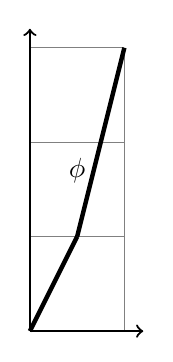
\begin{tikzpicture}[scale=1.2]
\draw[step=1,gray,very thin] (0,0) grid (1,3);
\draw [thick,->] (0,0) -- (1.2,0);
\draw [thick,->] (0,0) -- (0,3.2);
\draw [domain=0:0.5, ultra thick] plot (\x, 2*\x);
\draw [domain=0.5:1, ultra thick] plot (\x, 4*\x-1);
\draw (0.5,1.7) node {$\phi$};
\end{tikzpicture}
\qquad
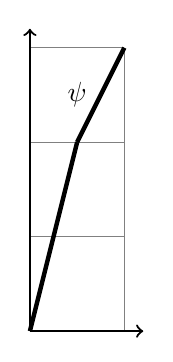
\begin{tikzpicture}[scale=1.2]
\draw[step=1,gray,very thin] (0,0) grid (1,3);
\draw [thick,->] (0,0) -- (1.2,0);
\draw [thick,->] (0,0) -- (0,3.2);
\draw [domain=0:0.5, ultra thick] plot (\x, 4*\x);
\draw [domain=0.5:1, ultra thick] plot (\x, 2*\x+1);
\draw (0.5,2.5) node {$\psi$};
\end{tikzpicture}
}
\begin{align*}
\phi\colon t& \mapsto \begin{cases}
4t & t\in [0,\frac12]\\
2t+1 & t\in [\frac12,1]
\end{cases}\\
\psi\colon t& \mapsto \begin{cases}
2t & t\in [0,\frac12]\\
4t-1 & t\in [\frac12,1]
\end{cases}
\end{align*}
with graphs as at right.

These two paths $I\to [0,3]$ are homotopic fixing endpoints by the homotopy $h_a(s,t) = 
s\phi(t) + (1-s) \phi(t)$. If we then precompose 
$\langle\gamma,\eta,\lambda\rangle\colon [0,3]\to X$ with $h_a\colon I\times I \to [0,3]$, 
we get a homotopy between $( \gamma \# \eta ) \# \lambda$ and $\gamma \# ( \eta 
\# \lambda)$. Path concatenation in $X$ is then \emph{homotopy associative}. But what 
about inverses or an identity element? We will play the same trick, by considering a 
`universal' case.

Given a path $\gamma\colon I \to X$, we have the reverse path $-\gamma$,
\marginnote{recall $-\gamma(t) := \gamma(1-t)$\\%} 
%\marginnote{%
\noindent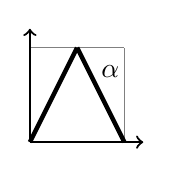
\begin{tikzpicture}[scale=1.2]
\draw[step=1,gray,very thin] (0,0) grid (1,1);
\draw [thick,->] (0,0) -- (1.2,0);
\draw [thick,->] (0,0) -- (0,1.2);
\draw [domain=0:0.5, ultra thick] plot (\x, 2*\x);
\draw [domain=0.5:1, ultra thick] plot (\x, 2-2*\x);
\draw (0.85,0.75) node {$\alpha$};
\end{tikzpicture}
\qquad
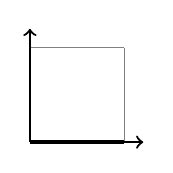
\begin{tikzpicture}[scale=1.2]
\draw[step=1,gray,very thin] (0,0) grid (1,1);
\draw [thick,->] (0,0) -- (1.2,0);
\draw [thick,->] (0,0) -- (0,1.2);
\draw [domain=0:1, ultra thick] plot (\x, 0);
% \draw [domain=0.5:1, ultra thick] plot (\x, 2-2*\x);
\end{tikzpicture}

\medskip

\noindent
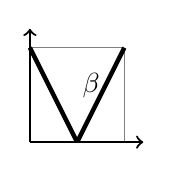
\begin{tikzpicture}[scale=1.2]
\draw[step=1,gray,very thin] (0,0) grid (1,1);
\draw [thick,->] (0,0) -- (1.2,0);
\draw [thick,->] (0,0) -- (0,1.2);
\draw [domain=0:0.5, ultra thick] plot (\x, 1-2*\x);
\draw [domain=0.5:1, ultra thick] plot (\x, 2*\x-1);
\draw (0.65,0.6) node {$\beta$};
\end{tikzpicture}
\qquad
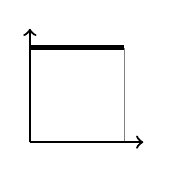
\begin{tikzpicture}[scale=1.2]
\draw[step=1,gray,very thin] (0,0) grid (1,1);
\draw [thick,->] (0,0) -- (1.2,0);
\draw [thick,->] (0,0) -- (0,1.2);
\draw [domain=0:1, ultra thick] plot (\x, 1);
% \draw [domain=0.5:1, ultra thick] plot (\x, 2-2*\x);
% \draw (0.5,2.5) node {$\psi$};
\end{tikzpicture}

\medskip

\noindent
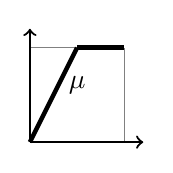
\begin{tikzpicture}[scale=1.2]
\draw[step=1,gray,very thin] (0,0) grid (1,1);
\draw [thick,->] (0,0) -- (1.2,0);
\draw [thick,->] (0,0) -- (0,1.2);
\draw [domain=0:0.5, ultra thick] plot (\x, 2*\x);
\draw [domain=0.5:1, ultra thick] plot (\x, 1);
\draw (0.5,0.6) node {$\mu$};
\end{tikzpicture}
\qquad
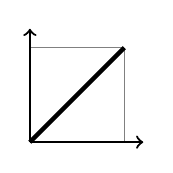
\begin{tikzpicture}[scale=1.2]
\draw[step=1,gray,very thin] (0,0) grid (1,1);
\draw [thick,->] (0,0) -- (1.2,0);
\draw [thick,->] (0,0) -- (0,1.2);
\draw [domain=0:1, ultra thick] plot (\x, \x);
% \draw [domain=0.5:1, ultra thick] plot (\x, 2-2*\x);
% \draw (0.5,2.5) node {$\psi$};
\end{tikzpicture}

\medskip

\noindent
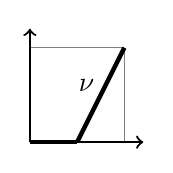
\begin{tikzpicture}[scale=1.2]
\draw[step=1,gray,very thin] (0,0) grid (1,1);
\draw [thick,->] (0,0) -- (1.2,0);
\draw [thick,->] (0,0) -- (0,1.2);
\draw [domain=0:0.5, ultra thick] plot (\x, 0);
\draw [domain=0.5:1, ultra thick] plot (\x, 2*\x-1);
\draw (0.6,0.6) node {$\nu$};
\end{tikzpicture}
\qquad
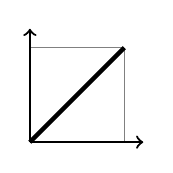
\begin{tikzpicture}[scale=1.2]
\draw[step=1,gray,very thin] (0,0) grid (1,1);
\draw [thick,->] (0,0) -- (1.2,0);
\draw [thick,->] (0,0) -- (0,1.2);
\draw [domain=0:1, ultra thick] plot (\x, \x);
% \draw [domain=0.5:1, ultra thick] plot (\x, 2-2*\x);
% \draw (0.5,2.5) node {$\psi$};
\end{tikzpicture}}
%
and the composite $\gamma \# (-\gamma)\colon I \to X$ can be factored as 
$I\xrightarrow{\alpha} I \xrightarrow{\gamma} X$ for a certain path $I\xrightarrow{\alpha} 
I$. If we instead concatenate in the other direction, namely $(-\gamma)\# \gamma\colon 
I\to X$, then this factors as $I\xrightarrow{\beta} I\xrightarrow{\gamma}X$. Again 
$\beta$ is a certain path in $I$. The graphs of both $\alpha$ and $\beta$ are shown at 
right, and both of them are homotopic, fixing endpoints, to the constant functions at 
$0$ and $1$ respectively, by taking an affine combination as in the definition of $h_a$ 
above. Then by composing the homotopies here with $\gamma$, we get homotopies between 
the path $\gamma\#(-\gamma)$ and the constant path at $\gamma(0)$, and also between 
$(-\gamma)\#\gamma$ and the constant path at $\gamma(1)$. So we have \emph{homotopy 
inverses}.

If we want to think about a homotopy identity element, then we should use the constant 
path $c_x\colon I\to X$ at a point $x\in X$, with $c_x(t)= x$, $\forall t\in I$. We can 
factor the composite $\gamma\# c_{\gamma(1)}$ as $I\xrightarrow{\mu} I 
\xrightarrow{\gamma} X$ for $\mu$ as shown at right, and factor $c_{\gamma(0)}\#\gamma$ 
as $I\xrightarrow{\nu} I \xrightarrow{\gamma} X$. As above, $\mu$ and $\nu$ are 
homotopic, fixing endpoints, to the identity map $I\to I$.

If we turn the five homotopies $I\times I \to X$ described above into paths $I\to X^I$, then if we start from elements of $\Omega_x X$, these homotopies correspond to paths in $\Omega_x X$.
Thus $\Omega_x X$, which has a concatenation binary operator $\#\colon \Omega_xX \times \Omega_xX\to \Omega_xX$, acts like a group, except the group axioms only hold up to the existence of paths\marginnote{More is true, though we won't prove it: there are homotopies assembled out of these paths for all possible cases, for instance $I \times \Omega_x X \times \Omega_x X \times \Omega_x X \to \Omega_x X$} 
\begin{align*}
( \gamma \# \eta ) \# \lambda & \rightsquigarrow \gamma \# ( \eta \# \lambda)\\
\gamma\# (-\gamma) &\rightsquigarrow c_{\gamma(0)}\\
(-\gamma)\# \gamma &\rightsquigarrow c_{\gamma(1)}\\
\gamma\# c_{\gamma(1)}&\rightsquigarrow \gamma \\
c_{\gamma(0)}\#\gamma &\rightsquigarrow \gamma
\end{align*}
in $\Omega_x X$. As a result we have proved most of

\begin{prop}
Let $(X,x)$ be a pointed space, with $X$ slsc.\marginnote{If we fall back on the default, namely just slpc, then we can use $[\pt,\Omega_x X]$ instead} The set $\pi_0(\Omega_x X)$ carries the 
structure of a group, its product arising from concatenation of loops and identity element 
represented by the constant path at $x$.
\end{prop}

\begin{proof}
To exhibit the multiplication, consider the functor $\pi_0$ applied\marginnote{This requires knowing that $\#$ is continuous! See Assignment 2.} to $\#\colon \Omega_x X 
\times \Omega_x X \to \Omega_x X$, giving $\pi_0(\Omega_x X \times \Omega_x X) \xrightarrow{\#} 
\pi_0(\Omega_x X)$. But since $\pi_0(M\times N) \xrightarrow{\simeq} 
\pi_0(M)\times\pi_0(N)$, for all slpc spaces $M$ and $N$, we get a composite 
$\pi_0(\Omega_x X) \times \pi_0(\Omega_x X) \simeq \pi_0(\Omega_x X \times \Omega_x X) 
\to \pi_0(\Omega_x X)$. This is associative and unital, and inverses exist, by the 
existence of the paths above.
\end{proof}

\begin{definition}
For\marginnote{Recall we also proved $[\pt,-]$ descends to a functor $\Ho \to \Set$ in Assignment 1}
 $(X,x)$ a pointed space its \emph{fundamental group at $x$} is 
$\pi_1(X,x) := [\pt,\Omega_xX]$, which for $X$ a slsc space coincides with $\pi_0(\Omega_xX)$.
\end{definition}

From\marginnote{As a point of clarification, everything here works for arbitrary slpc spaces with small adjustments, but for slsc spaces the approach is slightly cleaner, as components and path components coincide for the function spaces} the previous reasoning, we have constructed from a covering space $Z\to X$ and 
chosen basepoint $x\in X$ a permutation representation $\pi_1(X,x) \to \Aut(Z_x)$. If 
$Z$ is path connected, and we choose $z\in Z_x$, we get a surjective map $\pi_1(X,x) \to 
Z_x$, given by $\gamma\mapsto \gamma_*(z)$. This implies we have an upper bound on the 
cardinality of fibres of any path connected covering space, and conversely, given a 
connected covering space, the fibres give a lower bound on the number of distinct 
homotopy classes of loops in $X$.

\begin{example}
The projection map $S^2 \to \mathbb{RP}^2$ is a covering space and $S^2$ is connected, 
so there exist at least two non-homotopic loops in $\mathbb{RP}^2$ at any given 
basepoint. One of these is the constant loop, so there exists a loop in $\mathbb{RP}^2$ 
not homotopic to it.
\end{example}

\begin{example}\label{eg:piS^1_infinite}
We have the covering space $\exp(2\pi i-)\colon \RR\to S^1$ with fibre
$\ZZ$ over $1\in S^1$, which implies $\pi_1(S^1,1)$ is an infinite group.
\end{example}

\begin{prop}
The loop space construction is a functor $\Omega\colon \Top_*\to \Top_*$.
\end{prop}


\begin{corollary}
The fundamental group\marginnote{Exercise: This functor is naturally isomorphic to $[(S^1,1),(X,x)]_*$} gives a functor 
\[
	\pi_1 := [\pt,-] \circ \Omega\colon \Top_*\to \Grp.
\]
which for slsc spaces is naturally isomorphic to $\pi_0\circ \Omega$.
\end{corollary}


However,\lecturenum{8} as we have seen, we don't just get an action of $\pi_1(X,x)$ on the fibre $Z_x$ 
of a covering space. We also get what looks like an action of paths between different 
points on fibres, but now points in one fibre are taken to points of another fibre. In 
fact, if $X$ is not equipped with a basepoint to start with, or there are several 
natural options and no one of those is canonical, then we can create an even richer 
invariant, namely a \emph{groupoid}.

\begin{definition}
A \emph{groupoid} is a category where every morphism has an inverse.
\end{definition}

So that we have an idea of what kinds of groupoids arise, let us consider some examples. 
We will be considering only \emph{small} groupoids: those locally small groupoids 
$\Gamma$ where there is a set $\Gamma_0$ of objects. We can then take the disjoint union 
of all the hom-sets to get the set $\Gamma_1= \bigsqcup_{x,y\in \Gamma_0} \Gamma(x,y)$ of morphisms, and specify the source and 
target functions $s,t\colon \Gamma_1\rightrightarrows \Gamma_0$. Groupoids and functors 
form a category $\Gpd$.

\begin{example}
\begin{enumerate}
\item Every set $S$ gives a groupoid $\disc(S)$, by taking the set of objects to be $S$, and to only have identity
morphisms. This gives a full subcategory inclusion $\disc\colon \Set \into \Gpd$, and such groupoids are called \emph{discrete}.
\item Every set $C$ also gives another groupoid $\codisc(C)$ with set of objects $C$, but with exactly 
one morphism from any object to any other object. The set of morphisms is $C\times C$, and every 
object $c\in C$ has the trivial group of automorphisms. Such groupids are called \emph{codiscrete}.
\item Let $G$ act on the set $Y$ on the right. Then there is a groupoid $Y/\!/G$ with object set $Y$, and set of 
morphisms $Y\times G$. The source and target are given by $s(y,g)=y$, $t(y,g)=yg$, and composition is $(y,g)(yg,h) = (y,gh)$.
\begin{enumerate}
\item If $G=1$, then this recovers the first example.
\item If $Y=\pt$, then the information in the groupoid is essentially just that of the group $G$. Groupoids of this form will be denoted $\BB G$, and $\BB\colon \Grp \into \Gpd$ is the inclusion of a full subcategory.
\end{enumerate}
\end{enumerate}
\end{example}

A slogan people sometimes use is that a groupoid is like a group with `many identities', 
but you can also usefully think of them as being a generalisation of a group action, 
where you have different groups acting on different parts of the set. Here is a useful 
lemma about the structure of groupoids.

\begin{lemma}
For any groupoid $\Gamma$, and given $x,y\in \Gamma_0$,\marginnote{using algebraic order of composition}
\begin{align*}
	\Ad_a\colon \Gamma(x,x) & \xrightarrow{\simeq} \Gamma(y,y)\\
			g & \mapsto a^{-1}ga
\end{align*}
is an isomorphism for any $a\in \Gamma(y,x)$\marginnote{$(\Ad_a)^{-1} = \Ad_{a^{-1}}$\\\bigskip\noindent transitive: $(ba^{-1},a) \mapsto b$;\\ 
\noindent free: $ga=a$ implies $g = gaa^{-1} = aa^{-1} =\id_x$} and 
the function
\begin{align*}
	\Gamma(x,x)\times \Gamma(x,y) & \to \Gamma(x,y)\\
		(g,a) & \mapsto ga
\end{align*}
defines a free and transitive action of the group $\Gamma(x,x)$.
\end{lemma}

As a reminder: a free group action $G\times S\to S$ is one where $g\cdot p = p$ implies 
$g$ is the identity element, and a transitive action one where given any two elements 
$p,q\in S$, there is some group element $g\in G$ such that $g\cdot p = q$.

\begin{definition}
Given an slsc space $X$ and a specified subset $A\subseteq X$, the \emph{fundamental groupoid 
based at $A$}
is the groupoid $\Pi_1(X,A)$ with set of objects $A$, and the set of morphisms from $x$ to $y$ is $\Pi_1(X,A)(x,y) := \pi_0(P_x^yX)$. 
The\marginnote{the definition makes sense for more general slpc spaces, using $[\pt,-]$ in place of $\pi_0$, but we are only consider slsc spaces here} composition map is induced from concatenation of paths:
\[
	\pi_0(P_x^yX) \times \pi_0(P_y^zX) \simeq \pi_0(P_x^y X\times P_y^zX) \to \pi_0(P_x^zX)
\]
and 
constant paths are the identity morphisms.
\end{definition}


As with other invariants, the fundamental groupoid is a functor. Define the category 
$\Top^{(2)}$ to be the category with objects pairs $(X,A)$ where $X$ is a topological 
space and $A\subseteq X$ is a subspace, and a morphism $(X,A) \to (Y,B)$ is a continuous 
function $f\colon X\to Y$ such that $f(A) \subseteq B$. We have a full subcategory inclusion 
$\Top_*\into \Top^{(2)}$.

\begin{prop}
The fundamental groupoid gives a functor $\Pi_1\colon \Top^{(2)}\to \Gpd$ such that
\[
	\xymatrix{
		\Top_* \ar[r]^{\pi_1} \ar[d] & \Grp \ar[d]^{\BB}\\
		\Top^{(2)} \ar[r]_{\Pi_1} & \Gpd
	}
\]
and moreover:\marginnote{The product/disjoint union of groupoids is 
what you think it is: take the products/disjoint unions of the objects and the morphisms, respectively} 
\begin{align*}
	\Pi(X\times Y,A\times B) & \xrightarrow{\simeq} \Pi_1(X,A) \times \Pi_1(Y,B)\\
	\Pi_1(X,A) \sqcup \Pi_1(Y,B) & \xrightarrow{\simeq} \Pi(X\sqcup Y,A\sqcup B)
\end{align*}
\end{prop}

We can include \emph{unbased} spaces $X$ into pairs, by taking $(X,X)$, giving another 
fully faithful functor, $\Top \to \Top^{(2)}$. In this case, if the space $X$ has 
\emph{no} preferred basepoints whatsoever, we can still define the fundamental groupoid 
of $X$ itself as $\Pi_1(X,X)$, which is a functor $\Top \to \Gpd$.


We haven't yet seen how to calculate the fundamental group(oid) in 
examples, so we will turn to that now. We need a name for spaces $X$ that have 
$\Pi_1(X)$ trivial, in the sense of being codiscrete.

\begin{definition}
A space $X$ that satisfies $\Pi_1(X) = \codisc(X)$\marginnote{such spaces 
also have $\Pi_1(X,A) = \codisc(A)$ for all $A\subseteq X$} is called 
\emph{simply-connected}.
\end{definition}

If we unpack this definition, it tells us that a) given any two points $x,y\in X$, there is a (homotopy class of some) path from $x$ to $y$, so that $X$ is path-connected, and b) all paths between any two given points are endpoint-fixed homotopic, hence a unique morphism in the fundamental groupoid. 
As a result, $\pi_1(X,x) = \Pi_1(X)(x,x)$ is the trivial group.

\begin{example}
Convex subspaces $C\subseteq \RR^n$ are simply-connected, because any two points $v,w\in C$ 
can be joined by a path in $C$, and given two paths $\gamma,\eta\colon v\rightsquigarrow w$
the map $(s,t)\mapsto s\gamma(t)+(1-s)\eta(t)$ is a homotopy between them.
\end{example}

In particular, the interval $I$ is simply-connected. The fundamental groupoid $\Pi_1(I,\{0,1\})$
is important enough to have its own name: $\mathbf{2}$, sometimes denoted 
$(0\xrightarrow{\sim} 1)$, as it has two objects $0,1$ and a unique isomorphism between them.

\begin{ex}
Define a \emph{star-shaped region}\marginnote{For $\mathcal{H} \subset \CC$ the
(open) upper half-plane, the set $\mathcal{H}\cup\mathbb{Q}$ is star-shaped, but not convex} 
in a (real or complex) vector space $V$ to be a set 
$K\subseteq V$ such that there is a point $v_0\in K$ such that for every $v\in K$ and $t\in I$,
$tv_0+(1-t)v\in K$. Prove that star-shaped regions are simply-connected.
\end{ex}

Simply-connected spaces are special for the following reason.

\begin{prop}
If $X$ is a simply-connected space, then every path connected covering space 
$Z\xrightarrow{\pi} X$ is trivial, in the sense that $\pi$ is a homeomorphism.
\end{prop}

\begin{proof}
Recall that $\pi_1(X,x) \to Z_x$ is surjective for any $x\in X$, so $X$ simply-connected implies
$Z_x = \pt$ for all $x$. Thus $\pi$ is a bijection. The local triviality condition implies 
that every $x\in X$ has an open set $U\ni x$ such that $\pi^{-1}(U) \to U$ is a homeomorphism. 
Letting $U_\alpha$ range over such an cover of $X$, we can glue the inverses of these local 
homeomorphisms into a into an inverse for $\pi$.
\end{proof}



\begin{example}
If $X$ is contractible then it is simply-connected. Let $H\colon I\times X \to X$ be a 
contraction to $x_0\in X$. Consider the induced map $h= \Pi_1(H)\colon \Pi_1(I\times X, 
\{0,1\}\times X) \to \Pi_1(X,X) = \Pi_1(X)$. The domain simplifies to be 
$\Pi_1(I,\{0,1\})\times \Pi_1(X) = \mathbf{2}\times \Pi_1(X)$. Consider the induced maps 
$\{i\}\times \Pi_1(X)\to \mathbf{2}\times \Pi_1(X) \to \Pi_1(X)$ for $i=0,1$. Since 
$H\big|_{\{0\}\times X}=\id_X$, so $h_{\{0\}\times \Pi_1(X)}=\id_{\Pi_1(X)}$; and as 
$H\big|_{\{1\}\times X}$ is constant at $x_0$, so $h(0,x) = x_0$ for all $x\in X$, and 
$h\big|_{\{1\}\times \Pi_1(X)}$ sends every path to the constant path at $x_0$. We 
already know that $X$ is path connected, so that for any $x,y\in X$ there is some path 
between them. Given a path $\gamma\colon x\rightsquigarrow y$ consider the commutative square
\[
	\xymatrix{
	(0,x) \ar[r]^{(\id_0,[\gamma])} \ar[d] & (0,y) \\
	(1,x) \ar[r]_{(\id_1,[\gamma])} & (1,y) \ar[u]
	}
\]
in $\mathbf{2}\times \Pi_1(X)$ (recall all morphisms are invertible). Under $h$ this is sent to
\[
	\xymatrix{
	x\ar[r]^{[\gamma]} \ar[d] & y \\
	x_0 \ar[r]_{\id} & x_0 \ar[u]
	}
\]
The vertical arrows are independent of $[\gamma]$, so that every path $\gamma$ in $X$ is 
homotopic to the composite the long way around the square, hence to every other path.
\end{example}

So\lecturenum{9} in some sense, we are interested in spaces that are path connected, though this is 
useful when building spaces out of disjoint components. Here is another way we can get 
information about the fundamental groupoid of a space from the fundamental groupoid of 
other spaces.

\begin{theorem}\label{thm:cov_space_gives_faithful_functor}
Let $Z\xrightarrow{\pi} X$ be a covering space.\marginnote{thus the funtor $\Pi_1(\pi)$ is \emph{faithful}} 
Then $\Pi_1(Z)(z_1,z_2) \to \Pi_1(X)(\pi(z_1),\pi(z_2))$ is injective for all $z_1,z_2\in Z$.
\end{theorem}

We will prove this theorem in a little bit, but let us give an important result that follows.

\begin{corollary}
Given a covering space $(Z,z)\xrightarrow{\pi}(X,x)$, the induced homomorphism between fundamental groups identifies $\pi_1(Z,z)$ with a subgroup of 
$\pi_1(X,x)$.
\end{corollary}

This allows us, given a covering space whose fundamental groupoid we know, to place a 
lower bound on the size of the fundamental group of the base space. Alternatively, it 
places an upper bound on the size of the fundamental group of the covering space, so if 
$\pi_1(X,x)$ is finite, then so is $\pi_1(Z,z)$.

\begin{prop}\label{prop:cov_space_of_IxX}
Let $Z\to I\times X$ be a covering space. Then $Z\xrightarrow{\simeq} I\times Z_0$ over 
$I\times X$, where $Z_0 := Z_{\{0\}\times X}$.
\end{prop}

\begin{proof}
The function $Z\to I\times Z_0$ is given by $(\pr_1\circ \pi,\tau)$, for some 
$\tau\colon Z\to Z_0$, which we need to construct.
The idea is similar to the situation where we constructed the trivialisation of a 
covering space of $I$, which is the special case of $X=\pt$. 
Given $x\in X$, we get a trivisalisable covering space $Z_{I\times \{x\}}\to X$, and so 
a function $\tau_x\colon Z_{I\times \{x\}} \to I\times Z_{(0,x)} \xrightarrow{\pr_2}Z_{(0,x)}$. 
Hence we have a (potentially discontinuous) function $Z \to Z_0$ using the various $\tau_x$. 
We will write down a global version of this function using ingredients we already know to be 
continuous.

Given $(t,x)\in I\times X$, there is a path $(0,x) \rightsquigarrow (t,x)$ given by
$\eta_{(t,x)}(s) = (ts,x)$, which we want to vary continuously with $(t,x)$. We know that 
$I\times I \times X\to I\times X$, $(s,t,x) \mapsto (ts,x)$ is continuous, so that by the 
\begin{align*}
	I\times X & \to (I\times X)^I\\
	(t,x) & \mapsto \eta_{(t,x)}
\end{align*}
is continuous. We can now define the composite
\begin{align*}
	\tau\colon Z & \xrightarrow{\simeq} (I\times X)\times_{I\times X} Z \to (I\times X)^I \times_{I\times X} Z 
	\xrightarrow{\Lift} Z^I\xrightarrow{\ev_1} Z\\
	z&\mapsto (\pi(z),z)\qquad \mapsto\quad (-\eta_{\pi(z)},z)
\end{align*}
This map factors through $Z_0$, as if $(t,z) :=\pi(z)$, then $-\eta_z$ is a path in $I\times X$ 
from $(t,x)$ to $(0,x)$ and so the evaluation of the lift of $-\eta_z$ at $1$ sits over $(0,x)$.
Since all the maps here are continuous, $\tau$ is continuous.

We need to supply a continuous inverse to $(\pr_1\circ \pi,\tau)$, which is built the 
same way, except now using $\eta_z$ itself to lift, rather than $-\eta_z$:
\[
	\sigma\colon I\times Z_0 \to (I\times X)^I\times_{I\times X} Z \xrightarrow{\Lift}
	Z^I \xrightarrow{\ev_1} Z.
\]
This is manifestly continuous, and one can check that this map is the required inverse by
considering the composite at each point separately, where it reduces to considering $Z$ 
restricted to $I\times \{x\}$.
\end{proof}

\begin{corollary}\label{prop:pullback_by_homotopic_maps_iso}
If $f,g\colon X\to Y$ are homotopic, say by $H\colon I\times X \to Y$, and $Z\to Y$ is a 
covering space, then $f^*Z\simeq g^*Z$ over $X$.
\end{corollary}

\begin{proof}
If we form $H^*Z\to I\times X$, then we have by Proposition~\ref{prop:cov_space_of_IxX}
that $H^*Z \simeq I\times f^*Z$. But $g^*Z \to X$ is (isomorphic to)  
$(H^*Z)_{\{1\}\times X}$, hence is isomorphic to $(I\times f^*Z)_{\{1\}\times X}$, but this
is isomorphic to $f^*Z$.
\end{proof}

This gives us a criterion whereby we know that no interesting covering spaces exist

\begin{corollary}
If $X$ is contractible, then every covering space $Z\to X$ is isomorphic to $X\times Z_x$ 
for any $x\in X$.
\end{corollary}

\begin{proof}
Let $H\colon I\times X \to X$ be a contraction to $x\in X$\marginnote{Exercise: such a contraction exists for all $x\in X$}. Then for $c_x\colon X\to X$ the 
constant map at $x$, $c_x^*Z = X\times Z_x$. But $H$ is a homotopy between $\id_X$ and $c_x$,
and $\id^*Z = Z$, so by Corollary~\ref{prop:pullback_by_homotopic_maps_iso} we have the required
isomorphism.
\end{proof}

\begin{example}
Any locally convex topological vector space has no interesting covering spaces, likewise any convex or even star-shaped region therein.
The unit sphere in a separable, infinite-dimensional Hilbert space has no interesting covering
spaces. The infinite-dimensional Stiefel manifolds likewise.
\end{example}


\begin{corollary}
Let\marginnote{%
$\xymatrix{
\{0\}\times X \ar[d] \ar[r]^-{\widetilde{f}} & Z \ar[d]^\pi\\
I\times X \ar@{-->}[ur]^{\widetilde{H}} \ar[r]_-{H} &Y
}$}
$Z\xrightarrow{\pi} Y$ be a covering space, $f,g\colon X\to Y$ a pair of maps and 
$H\colon I\times X\to Y$ a homotopy from $f$ to $g$. If $\widetilde{f}\colon \{0\}\times 
X\to Z$ is a lift of $f$, in the sense that the diagram at right commutes, then there is 
a unique homotopy $\widetilde{H}\colon I\times X \to Z$ lifting $H$ from $\widetilde{f}$ 
to a lift of $g$.
\end{corollary}

\begin{proof}
Since $I\times f^*Z \xrightarrow{\simeq} H^*Z$, and we have a section $X\to f^*Z$, then 
we get a section $I\times X \to I\times f^*Z$. Composing with the isomorphism we get a 
map $I\times X \to I\times f^*Z \to H^* Z \to Z$, and this both restricts to 
$\widetilde{f}$ on $\{0\}\times X$ and covers $H$. To show uniqueness, notice that 
$H(-,x)$ gives a path in $Y$ for each fixed $x\in X$. Any lift $\widetilde{H}'$ of $H$ 
likewise gives a path $\widetilde{H}'(-,x)$ for fixed $x$. Since lifts of paths are unique, the 
$\widetilde{H}'(-,x)$ must agree with $\widetilde{H}(-,x)$ for all $x$, hence 
$\widetilde{H}'=\widetilde{H}$.
\end{proof}

We can now give the promised proof of Theorem~\ref{thm:cov_space_gives_faithful_functor}.

\begin{proof}
(of Theorem~\ref{thm:cov_space_gives_faithful_functor}) Given paths $\gamma,\eta\colon z_1 \rightsquigarrow z_2$ in $Z$, and an endpoint-fixing homotopy 
$H\colon I\times I \to X$ between $\pi\circ \gamma$ and $\pi\circ\eta$, we can lift $H$ to give
a homotopy from $\gamma$ to a lift of $\pi\circ \eta$. Since $H$ fixes endpoints, the lifts of
the constant paths $H\big|_{I\times\{i\}}$, for $i=0,1$ are path in the fibre, discrete spaces.
Hence these paths are constant, and $\widetilde{H}$ is a homotopy fixing endpoints.
Since $\eta$ is a lift of $\pi\circ \eta$, unique path lifting gives that $\widetilde{H}$ is 
in fact a homotopy (fixing endpoints) from $\gamma$ to $\eta$. Thus $\gamma$ and $\eta$ give
the same element in $\Pi_1(Z)(z_1,z_2)$, and the induced map in injective as required. 
\end{proof}

Until now, a lot of our resuls only give bounds on or estimates between the fibres of a covering
space and the fundamental group of the base space. However, we can actually get an exact result, given a certain kind of covering space

\begin{theorem}
If $\pi\colon (Z,z) \to (X,x)$ is a covering space with $Z$ path connected, then  
\[
Z_x \simeq \pi_1(X,x)/\pi_1(Z,z),
\]
as sets with $\pi_1(X,x)$-action.
\end{theorem}

\lecturenum{10}

\begin{proof}

There\marginnote{For a group $G$, sets with a $G$-action will be called 
\emph{$G$-sets}.}  is in fact a canonical isomorphism, induced in the following way. For 
group $G$ and any transitive $G$-set $S$, and a point $p\in S$, then the map $G \to S$, 
$g\mapsto g\cdot s$ induces a well-defined bijection $G/\mathrm{Stab}(s) \to S$, where 
$\mathrm{Stab}(s) < G$ is the subgroup of elements $g$ such that $g\cdot s = s$ (the 
\emph{stabiliser subgroup}). Notice that for \emph{any} subgroup $H< G$, $G/H$ inherits 
a $G$-action from the multiplication in $G$. And the bijection $G/\mathrm{Stab}(s) \to S$ is 
compatible with the $G$-actions\marginnote{that is, \emph{equivariant}}.

We apply this to the transitive $\pi_1(X,x)$-set $Z_x$, where we know the action is 
transitive as $Z$ is path-connected. This gives an isomorphism 
$\pi_1(X,x)/\mathrm{Stab}(z) \xrightarrow{\simeq} Z_x$, and it remains to identify 
$\mathrm{Stab}(z) < \pi_1(X,x)$. But note that if for some $[\gamma] \in \pi_1(X,x)$, 
$\gamma_*(z)=z$, this means that the lift $\widetilde{\gamma_z}$ beginning at $z$ also 
ends at $z$, so is a loop in $Z$. Thus $\mathrm{Stab}(z)$ consists of the homotopy 
classes of loops in $X$ that come from loops in $Z$, that is, $\mathrm{Stab}(z) = 
\pi_1(Z,z)$.
\end{proof}




\begin{corollary}\label{cor:fibre_of_univ_cov_space}
If $\pi\colon (Z,z) \to (X,x)$ is a covering space with $Z$ simply-connected, then the map
\[
\pi_1(X,x) \to Z_x
\]
is an isomorphism of $\pi_1(X,x)$-sets.
\end{corollary}


\begin{proof}
Since $Z$ is simply-connected, $\pi_1(Z,z) = 1$, and so $\pi_1(X,x) \to Z_x$ is an isomorphism
of sets with $\pi_1(X,x)$-action.
\end{proof}

\begin{example}
We now can say that $\pi_1(S^1,1)$ is not just infinite (see Example~\ref{eg:piS^1_infinite})
 but countable, since it is in bijection with the fibre $\ZZ$ of the simply-connected covering space $\RR \to S^1$.
\end{example}

But even better, we have not just a bijection, but Corollary 
\ref{cor:fibre_of_univ_cov_space} gives a \emph{faithful permutation representation}: 
given $[\gamma],[\eta]\in \pi_1(X,x)$, there is some $z\in Z_x$ such that 
$\gamma_*(z)\neq \eta_*(z)$, which is equivalent to $\pi_1(X,x) \to \Aut(Z_x)$ being 
injective. Thus we have represented the fundamental group of $(X,x)$ as a permutation 
group, where we can do more concrete computations.

\begin{corollary}
For $(Z,z)\to (X,x)$ a simply-connected covering space, $\pi_1(X,x)$ acts freely on $Z_x$.
\end{corollary}

And now we can give the first example of an actually calculated, non-trivial fundamental group.

\begin{theorem}
$\pi_1(S^1,1) \simeq \ZZ$.
\end{theorem}

\begin{proof}
We have the simply-connected covering space $\RR \to S^1 = \RR/\ZZ$, with fibre over 
$1\in S^1$ being the integers. The inclusion $[0,1]\to \RR$ is a lift of the loop $\gamma$ 
going once around the circle, and all lifts are translates of this, so that the action of 
$\gamma$ on the fibre $\ZZ$ is translation by $1$. The loop $\gamma$ generates a subgroup
whose action on $\ZZ$ is transitive, hence $\gamma$ generates all of $\pi_1(S^1,1)$,
which must then be infinite cyclic, hence $\ZZ$.
\end{proof}

As a result, for any subset $A\subset S^1$, the fundamental groupoid $\Pi_1(S^1,A)$ has as 
objects the set $A$, for every $x\in A$, $\pi_1(S^1,x) \simeq \ZZ$, and for any two points
$x,y\in S^1$, the hom-set $\Pi_1(S^1,A)(x,y)$ is isomorphic as a set to $\ZZ$.


But how do we calculate $\pi_1$ in general? Or better, $\Pi_1$? Recall that $\Pi_1(X,A) = \Pi_1(X_1,A\cap X_1) \sqcup
\Pi_1(X_2,A\cap X_2)$.
For instance, if $X_1$ and $X_2$ are the only path components of $X$, and 
$\exists x\in A\cap X_i$ for $i=1,2$, then every point in $X$ is connected by a path to a point
in $A$. This means the fundamental goups of the two path components are captured.

\begin{example}
Consider $\Pi_1(S^1\sqcup S^1,1\sqcup 1)$, which is a groupoid with two objects, both of which
have automorphism groups given by $\ZZ$.
\end{example}

So we are going to focus a bit on calculating the fundamental group(oid) for path 
connected spaces. The easiest way to make a new connected space from two other connected spaces $X,Y$, say\marginnote{recall that we are taking spaces to be semilocally path connected, so that components and path components coincide}, is to take a point in each, $x\in X$, $y\in Y$, and identify $x$ and $y$.

\begin{definition}
Given\marginnote{A key property of the join is that given a pointed space $(M,m)$ and a pair of pointed 
maps $f\colon (X,x) \to (M,m)$, $g\colon (Y,y) \to (M,m)$, there is a unique pointed map 
$\langle f,g\rangle\colon (X\vee Y,\ast) \to (M,m)$ such that $f = \mathrm{in}_L\circ 
\langle f,g\rangle$ and $g = \mathrm{in}_R\circ \langle f,g\rangle$.} two pointed spaces $(X,x)$ and $(Y,y)$, the \emph{join} $X\vee Y$ is the quotient 
space $(X\sqcup Y)/(x\sim y)$. It has a basepoint given by $*:=[x] = [y]$, and the 
inclusion maps of $(X,x)\xrightarrow{\mathrm{in}_L} (X\vee Y,*) \xleftarrow{\mathrm{in}_R} (Y,y)$ are pointed.
\end{definition}



Since we have pointed maps, we get from functoriality of $\pi_1$ two 
homomorphisms $\pi_1(X,x) \to \pi_1(X\vee Y,*) \leftarrow \pi_1(Y,y)$. 
If we already know what the fundamental groups of $X$ and $Y$ are, then we 
can try to leverage this knowledge to tell us something about the fundamental group
of the join. For instance, taking $X = Y = S^1$, we get homomorphisms 
\[
\ZZ \xrightarrow{\pi_1(\mathrm{in}_L)} \pi_1(S^\vee S^1,\ast) \xleftarrow{\pi_1(\mathrm{in}_R)} \ZZ
\]
Let\marginnote{%
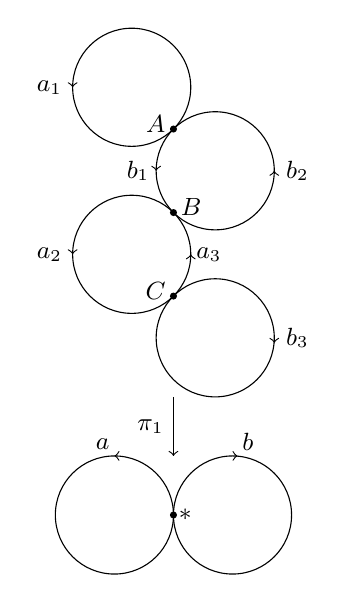
\begin{tikzpicture}[scale=1.5]
\draw[decoration={markings, 
                    % mark=at position 0 with {\arrow{>}};,
                    mark=at position 0.5 with {\arrow{>}}},
                    postaction={decorate}]
        ({-1/(2*sqrt(2))},{1.5+3/sqrt(2)}) circle (0.5);
\draw (-1.05,{1.5+3/sqrt(2)}) node {\small $a_1$};
\fill (0,{1.5+2.5/sqrt(2)}) circle (0.03);
\draw (-0.15,{1.9+2/sqrt(2)}) node {\small $A$};    

\draw[decoration={markings, 
                    mark=at position 0 with {\arrow{>}};,
                    mark=at position 0.5 with {\arrow{>}}},
                    postaction={decorate}]
        ({1/(2*sqrt(2))},{1.5+2/sqrt(2)}) circle (0.5);
\draw (-0.3,{1.5+2/sqrt(2)}) node {\small $b_1$};
\draw (1.05,{1.5+2/sqrt(2)}) node {\small $b_2$};
\fill (0,{1.5+1.5/sqrt(2)}) circle (0.03);
\draw (0.15,{1.9+1/sqrt(2)}) node {\small $B$};

\draw[decoration={markings, 
                    mark=at position 0 with {\arrow{>}};,
                    mark=at position 0.5 with {\arrow{>}}},
                    postaction={decorate}]
        ({-1/(2*sqrt(2))},{1.5+1/sqrt(2)}) circle (0.5);
\draw (0.3,{1.5+1/sqrt(2)}) node {\small $a_3$};
\draw (-1.05,{1.5+1/sqrt(2)}) node {\small $a_2$};
\fill (0,{1.5+0.5/sqrt(2)}) circle (0.03);
\draw (-0.15,{1.9}) node {\small $C$};        

\draw[decoration={markings, 
                    mark=at position 0 with {\arrow{<}}},
                    postaction={decorate}]
        ({1/(2*sqrt(2))},1.5) circle (0.5);
\draw (1.05,{1.5}) node {\small $b_3$};

\draw[->] (0,1) -- (0,0.5)  node[midway,left] {\small $\pi_1$} ;

\draw[decoration={markings, mark=at position 0.25 with {\arrow{>}}},postaction={decorate}]
        (-0.5,0) circle (0.5);
\draw (-0.6,0.6) node {\small $a$};
\draw[decoration={markings, mark=at position 0.25 with {\arrow{<}}},postaction={decorate}]
        (0.5,0) circle (0.5);
\draw (0.63,0.62) node {\small $b$};
\fill (0,0) circle (0.03);
\draw (0.1,0) node {\small $\ast$};


\end{tikzpicture}}
us define $a,b\in \pi_1(S^1\vee S^1,\ast)$ to be the classes $\pi_1(\mathrm{in}_L)(1)$ and
$\pi_1(\mathrm{in}_R)(1)$ respectively.

Define the covering space $Z_1 \xrightarrow{\pi_1} S^1\vee S^1$ as at right, where 
$A,B,C \mapsto \ast$, and $a_i\mapsto a$, $b_i\mapsto b$, $i=1,2,3$. Then we get a 
representation $\rho_1\colon \pi_1(S^1\vee S^1,\ast)\to \Aut\{A,B,C\} \simeq S_3$. 
Looking at how paths representing $a$ and $b$ lift, we get $\rho_1(a) = (BC)$ and 
$\rho_1(b) = (AB)$, cycles in $S_3$. Calculating $\rho_1(ab)$ we get $(ABC)$, and 
similarly for $\rho_1(ba)$, to get $(ACB)$, so that $rho_1(ab) \neq \rho_1(ba)$.
As a result, we must have had $ab \neq ba$ in $\pi_1(S^1\vee S^1,\ast)$, or in other words,
the fundamental group of $S^1\vee S^1$ is \textbf{non-abelian}.

By a judicious choice of covering spaces, we can also prove that the two homomorphism 
$\ZZ \to \pi_1(S^1\vee S^1,\ast)$ are injective, so that $a$ and $b$ generate infinite 
cyclic subgroups. We will\marginnote{We can present $\ZZ\ast\ZZ$ as $\langle a,b|\ 
\rangle$, which has as elements $a^{n_1}b^{m_1}\ldots a^{n_k}b^{m_k}$ for $k\geq 1$ and 
$n_i,m_i\in \ZZ$, with $a^0=e=b^0$} later prove that $\pi_1(S^1\vee S^1,\ast) \simeq 
\ZZ\ast \ZZ = F_2$, a free group on the generators $a,b$.


\lecturenum{11}

\begin{definition}
The \emph{free group on $n$-symbols}, $F_n$ is any group with presentation 
\[
	\langle x_1,\ldots,x_n\mid\ \rangle.
\]
That is, generators $x_1,\ldots,x_n$ and no relations.
\end{definition}

The symbols are of course arbitrary. Elements in $F_n$ are (finite) words in $x_i$ and $x_i^{-1}$, with the empty word $()$ being the identity element, and with concatenation of words being the multiplication in $F_n$.

\begin{definition}
Given groups $G$ and $H$, the \emph{free product} $G\ast H$ of $G$ and $H$ is a group equipped with homomorphisms $i\colon G\to G\ast H$, $j\colon H \to G\ast H$, satisfying the following property: given any group $K$ and homomorphisms $\phi\colon G \to K$, $\psi\colon H\to K$, there exists a unique homomorphism $\kappa\colon G\ast H \to K$ such that $\phi = i\circ \kappa$ and $\psi=j\circ \kappa$.
\end{definition}


We can write things like this:
\[
	\xymatrix{
		& H \ar[d]^j \ar@/^1pc/[rdd]^\psi &\\
		G \ar[r]^i \ar@/_1pc/[drr]_\phi & G\ast H \ar@{-->}[dr]^{\exists!}_\kappa &\\
		&& K
	}
\]
The existence of the unique $\kappa$ given the data of $\phi$ and $\psi$ is the \emph{universal property} of the free product.

If\marginnote{here each $R_i$ and $Q_j$ are \emph{relations}: equations involving the given generators of $G$ and $H$ respectively} $G = \langle g_1,\ldots,g_m\mid R_1,\ldots, R_n\rangle$  and $H = \langle h_1,\ldots, h_k \mid Q_1,\ldots, Q_l\rangle$ are presentations of $H$ and $G$, then
\[
	G\ast H = \langle g_1,\ldots,g_m,h_1,\ldots,h_k \mid R_1,\ldots, R_n,Q_1,\ldots,Q_l\rangle
\]


The free product of groups is an example of a more general construction, the \emph{free product with amalgamation}, but this is again an example of a general construction that makes sense in an arbitrary category.

\begin{definition}
Let $\cC$ be an arbitrary category. A \emph{pushout square} is a commutative square
\[
	\xymatrix{
		W\ar[r]^b \ar[d]_a & Y \ar[d]^d \\
		X \ar[r]_c & P
	}
\]
in $\cC$ such that for any pair of morphisms $X\xrightarrow{f} Z \xleftarrow{g} Y$ such that 
$f\circ a = g\circ b$,\marginnote{this unique existence is the \emph{universal property} of the pushout}
\[
	\exists!\ P\xrightarrow{k} Z \quad \text{such that} \quad  f=k\circ c \text{ and } g=k\circ d.
\]
\end{definition}

\begin{example}
Consider a topological space $X$, and $U,V \subseteq X$ subspaces such that the $\{U^o,V^o\}$ is an open cover of $X$. Then\marginnote{$U$ and $V$ here are `glued together' along $U\cap V$ to give $X$}
\[
	\xymatrix{
		U\cap V\ar[r] \ar[d] & V \ar[d] \\
		U \ar[r] & X
	}
\]
is a pushout square in $\Top$, where all maps are the inclusions.
\end{example}

In the above example, we call $\{U,V\}$ a cover of $X$ by nhds, since at least one of $U$ and $V$ is a nhd of each point in $X$.

\begin{example}
For any pair of pointed spaces $(X,x)$ and $(Y,y)$, 
\[
	\xymatrix{
		(\pt,\pt)\ar[r] \ar[d] & (Y,y) \ar[d]^{\mathrm{in}_R} \\
		(X,x) \ar[r]_-{\mathrm{in}_L} & (X\vee Y,\ast)
	}
\]
is a pushout square in $\Top_*$.
\end{example}

\begin{example}
For arbitrary groups $G$ and $H$,
\[
	\xymatrix{
		1\ar[r] \ar[d] & H \ar[d] \\
		G \ar[r] & G\ast H
	}
\]
is a pushout square in $\Grp$.
\end{example}

\begin{example}
Recall the groupoid $\mathbf{2}$ with two objects, $0$ and $1$ and a unique arrow between any ordered pair of objects. The square
\[
	\xymatrix{
		\disc(\{0,1\}) \ar[r] \ar[d] & \mathbf{2}\ar[d]^{(0\to 1)\mapsto (\bullet \xrightarrow{1} \bullet)} \\
		\pt \ar[r]&  \mathbb{B}\ZZ
	}
\]
is a pushout in $\Gpd$.
\end{example}

\begin{example}
Consider the category $\Vect$ of vector spaces (over some fixed field) and linear maps. The square
\[
	\xymatrix{
		W\ar[r]^{L_2} \ar[d]_{L_1} & V_2 \ar[d] \\
		V_1 \ar[r] & (V_1\oplus V_2)/J(W)
	}
\]
with $J\colon W\to V_1\oplus V_2$ the map $w\mapsto (L_1(w),-L_2(w))$ is a pushout.
\end{example}


\begin{theorem}[Seifert--van Kampen theorem]
Let $X$ be a space, and $\{U,V\}$ a cover by nhds. Then
\[
	\xymatrix{
		\Pi_1(U\cap V) \ar[r]^-{i_V} \ar[d]_{i_U} & \Pi_1(V) \ar[d]\\
		\Pi_1(U) \ar[r] & \Pi_1(X)
	}
\]
is a pushout square in $\Gpd$.
\end{theorem}

\begin{rem}
It is \textbf{not} immediate that this is a pushout just because the square of spaces is 
a pushout in $\Top$, because we need to check the universal property for arbitrary 
groupoids $\Gamma$ and (compatible) functors $\Pi_1(U) \to \Gamma \leftarrow \Pi_1(V)$.
\end{rem}


\begin{proof}
We need to start with an arbitrary commutative square
\[
	\xymatrix{
		\Pi_1(U\cap V) \ar[r]^-{i_V} \ar[d]_{i_U} & \Pi_1(V) \ar[d]^G\\
		\Pi_1(U) \ar[r]_-F & \Gamma
	}
\]
and construct a functor $K\colon \Pi_1(X) \to \Gamma$ compatible with $F$ and $G$. That 
is, we need to construct a pair of functions $K_0\colon \Pi_1(X)_0 = X \to \Gamma_0$ and 
$K_1\colon \Pi_1(X)_1 \to \Gamma_1$ that together define a functor as needed.

Firstly, consider arbitrary $x\in X$. If $x\in U$, then define $K_0(x) = F(x)$, and if 
$x\in V$, define $K_0(x) = G(x)$. If $x\in U\cap V$, then since $F\circ i_U = G\circ 
i_V$, $F(x) = G(x)$, and so $K_0$ is well-defined.

We will first define $K_1$ on actual paths, and then show it is invariant under passing 
to homotopy classes. Suppose that $\gamma\colon I\to X$ factors through $U \into X$. 
Then we can define $K_1(\gamma) = F_1(\gamma)$, and similarly, if it factors through 
$V\into X$, then define $K_1(\gamma) = G_1(\gamma)$. Again, if $\gamma$ lands in $U\cap 
V$ then it is unambiguously defined, by the commutativity of the square as given. This 
is compatible with source and target maps, since the start- and end-points of a path in 
$U$ lie in $U$, and similarly for $V$, and $F$ and $G$ are functors. It is compatible 
with concatenation of paths that lie entirely inside $U$ or inside $V$, again using the 
fact $F$ and $G$ are functors. Constant paths are sent by $K_1$ to identity morphisms in 
$\Gamma$, as needed, since they are by $F$ and $G$. Also notice that if we reparametrise 
the path $\gamma$ to $\gamma\circ \sigma$, this gives an equal morphism in $\Pi_1(U)$ or 
$\Pi_1(V)$ as appropriate, so that $K_1$ is independent of the parametrisation of the 
path.

We now need to consider a general path $\gamma\colon I\to X$ and define $K_1(\gamma)$. 
If we pull back the open cover $\{U^o,V^o\}$ along $\gamma$ to an open cover of $I$, we 
can find a partition\marginnote{using the Lebesgue covering lemma} $0=t_0<t_1<\ldots < 
t_n<t_{n+1}=1$ of $I$ such that for each $i=0,\ldots n$, $\gamma\big|_{[t_i,t_{i+1}]}$ 
factors through either $U\into X$ or $V\into X$ (or both). Define $\gamma_i \colon I 
\simeq [t_i,t_{i+1}] \to X$, so that $\gamma$ is homotopic to the concatenation of all 
the $\gamma_i$s, and in fact $\gamma$ is a reparametrisation of the concatenation. We 
have already defined $K_1(\gamma_i)$, so let $K_1(\gamma) = 
K_1(\gamma_0)K_1(\gamma_1)\cdots K_1(\gamma_n) \in \Gamma_1$. Note that by the 
compatibility of $K_1$ with concatenation \emph{inside $U$ and $V$}, if we pass to a 
finer partition of $I$, we get a different sequence $\gamma_j$, but the composite of the 
$K_1(\gamma_j)$s is equal to what we just defined. Since any two partitions have a 
common refinement, the definition of $K_1$ is independent of the choice of partition. 
Again, since the original given square commutes, there is no ambiguity when a given 
$\gamma_i$ factors through $U\cap V$.

We now need to show that given an endpoint-fixing homotopy $H\colon I\times I \to X$ 
between paths $\gamma$ and $\eta$, then $K_1$ maps them both to the same morphism in 
$\Gamma$.

Consider\marginnote{%
\begin{tikzpicture}
\fill (0,0) circle (0.05) node[anchor=east] {$h(0,0)$};
\draw[decoration={markings, mark=at position 0.75 with {\arrow{>}}},postaction={decorate}] 
		(0,0) -- (2,0) -- (2,2);
\draw (2,1) node[anchor=west] {$\gamma_0$};
\draw[decoration={markings, mark=at position 0.25 with {\arrow{>}}},postaction={decorate}] 
 		(0,0) -- (0,2) -- (2,2);
\draw (0,1) node[anchor=east] {$\gamma_1$};
\fill (2,2) circle (0.05) node[anchor=west] {$h(1,1)$};
\end{tikzpicture}
}
as a warmup, an arbitrary map $h\colon I^2\to X$, and define paths 
$\gamma_0,\gamma_1\colon h(0,0) \rightsquigarrow h(1,1)$ in $X$ as the concatenations
\begin{align*}
\gamma_0 & := h(-,0)\# h(1,-),\\
\gamma_1 & := h(0,-)\# h(-,1).
\end{align*}

Then there is an endpoint-fixing homotopy $\gamma_0 \sim \gamma_1$. It is sufficient to 
define an endpoint-fixing homotopy $I\times I \to I^2$ between the two paths around the 
square that arise from taking $h$ to be the identity map $I^2\to I^2$.
\begin{center}
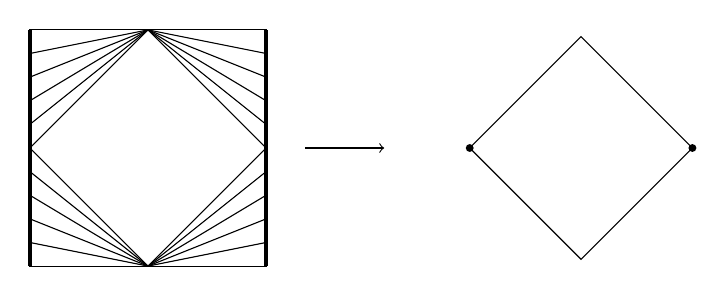
\begin{tikzpicture}
\draw (0,0) rectangle +(3,3);
\draw[ultra thick] (0,0) -- (0,3) (3,0) -- (3,3); 
\foreach \n in {1,...,5}
{
	\draw (1.5,0) -- (0,\n*1.5/5);
	\draw (1.5,0) -- (3,\n*1.5/5);
	\draw (1.5,3) -- (0,3-\n*1.5/5);
	\draw (1.5,3) -- (3,3-\n*1.5/5);
}
\draw[->] (3.5,1.5) -- (4.5,1.5);
\draw[rotate around={45:(7,1.5)}] (6,0.5) rectangle +(2,2);
\fill[rotate around={45:(7,1.5)}] (6,2.5) circle (0.05);
\fill[rotate around={45:(7,1.5)}] (8,0.5) circle (0.05);
\end{tikzpicture}
\end{center}

Here the function is constant on the vertical edges of the square at the two vertices, 
and on each diagonal line as shown maps to the corresponding edges of the square on the 
right.
Thus if $h$ factors through one of $U$ or $V$, $K_1(\gamma_0) = K_1(\gamma_1)$, since 
$[\gamma_0] = [\gamma_1]$ in one of $\Pi_1(U)$, $\Pi_1(V)$.

\lecturenum{12}

By\marginnote{%
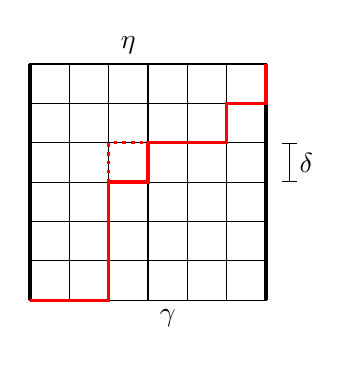
\begin{tikzpicture}
\draw (0,0) rectangle (3,3);
\draw (1.75,0) node[below] {$\gamma$};
\draw (1.25,3) node[above] {$\eta$};
\draw[ultra thick] (0,0) -- (0,3) (3,0) -- (3,3);
\foreach \x in {0,...,5}
{
	\foreach \y in {0,...,5}
	\draw (\x/2,\y/2) rectangle (\x/2+0.5,\y/2+0.5);
}
\draw[|-|] (3.3,1.5) -- node[right] {$\delta$}  (3.3,2);
\draw[very thick,red] (0,0) -- (1,0) -- (1,1.5) -- (1.5,1.5) -- (1.5,2) --
		(2.5,2) -- (2.5,2.5) -- (3,2.5) -- (3,3);
\draw[very thick,red,dotted] (1,1.5) -- (1,2) -- (1.5,2);
\end{tikzpicture}
} the Lebesgue covering lemma applied $(I^2,d_\infty)$ and the open cover 
$\{H^{-1}(U^o), H^{-1}(V^o)\}$, there is a some $\delta > 0$ such that every square of 
side-length $\leq\delta$ in $I^2$ (a \emph{$\delta$-square}) is contained in one of 
$H^{-1}(U^o)$ and $H^{-1}(V^o)$. Thus $H\big|_{[a,a+\delta]\times[b,b+\delta]}$ factors 
through one of $U$ or $V$, for any suitable $(a,b)\in I^2$. We then cover $I^2$ by such 
$\delta$-squares, noting that this also give a partition of $I$ into intervals such that 
both $\gamma$ and $\eta$ restricted to such intervals factor through one of $U$ or $V$, 
so that $K_1$ is defined on $\gamma$ and $\eta$.

Now we can use the fact about paths between opposite vertices of the square 
being\marginnote{all homotopies here will have fixed endpoints} homotopic to iteratively 
show that $K_1(\gamma) = K_1(\eta)$. Firstly, note that $\gamma$ is homotopic to the 
path gotten by concatenating with the constant path up the right side of the square, and 
similarly, $\eta$ is homopic to the path gotten by concatenating with the constant path 
up the left side of the square. Then the big homotopy is pasted together from homotopies 
that move one square at a time, each of which land in one of $U$ or $V$. Then the two 
possible red paths shown in the figure, for example, get mapped by $K_1$ to the same morphism 
in $\Gamma$. All up, these show that $K_1(\gamma) = K_1(\eta)$, and so $K_1$ is 
well-defined on homotopy classes of paths. By the construction of $K_1$, it preserves 
composition, so is functorial, and we are done.
\end{proof}

This is a powerful theorem, but sometimes not the best for computation, in this form. It 
would be good to have a version for more general $\Pi_1(X,A)$, for smaller $A\subset X$, 
or even $\pi_1(X,x)$. To do this, we need a general categorical lemma

Given\marginnote{%
$\xymatrix@!=2ex{
	A_1 \ar[rr] \ar[dd] \ar[dr] && B_1 \ar[dr] \ar[dd]|\hole\\
	& A_2 \ar[rr] \ar[dd] && B_2 \ar[dd]\\
	C_1\ar[dr] \ar[rr]|\hole && D_1\ar[dr] \\
	& C_2 \ar[rr] && D_2
}$\\
\noindent A morphism from the back square to the front square in $\cC^\square$} 
an arbitrary category $\cC$, we can define a category $\cC^\square$ with objects 
commutative squares in $\cC$, and morphisms commutative \emph{cubes}: cubes of objects 
and morphisms such that every face is a commutative square.

\begin{definition}
In a category $\cC$, an object $V$ is a \emph{retract} of an object $W$, if\marginnote{the morphism $r$ is called a \emph{retraction}} there are 
morphisms $i\colon V\to W$ and $r\colon W\to V$ such that $r\circ i = \id_V$.
\end{definition}

For example, in $\Vect$, any subspace $V$ of $\RR^n$ is a retract, by taking $i$ to be 
the inclusion, and $r$ to be orthogonal projection onto $V$. In $\Set$, given a set $S$ 
and a subset $T \subseteq S$ with some chosen $t_0\in T$ we get a retract given by the 
inclusion and the function $r\colon S\to T$ defined by $r(t) = t$, for $t\in T$, $r(s) = 
t_0$ for $s\in S\setminus T$. A more serious example is:
		
\begin{example}\label{eg:retracts_of_Pi1}
Given a space\marginnote{This generalises the case from Assignment 2, where $A'=\{x\}$} 
$X$, with subspaces $A' \subseteq A$ such that every point in $Aß$ is 
connected by a path in $X$ to a point in $A'$. Then $\Pi_1(X,A')$ is a retract of 
$\Pi_1(X,A)$. The case we will most care about is $A=X$, and various $A'\subseteq X$.
\end{example}

We can talk about what it means for a commutative square in a category $\cC$ to be a 
retract of another commutative square in $\cC$, by looking at retracts in $\cC^\square$. 
Recall that pushout squares are special examples of commutative squares. Also, to check 
that a morphism of commutative squares is a retraction, it is enough to check that it is 
a retraction at each vertex (that is, we have four retractions in $\cC$, one for each 
vertex of the square)

\begin{lemma}\label{lemma:retracts_of_pushouts}
Retracts of pushout squares are pushout squares.
\end{lemma}

\begin{proof}
Exercise.
\end{proof}

We wish to apply Lemma~\ref{lemma:retracts_of_pushouts} to the pushout square in 
$\Gpd$---hence an object of $\Gpd^\square$---from the Seifert--van Kampen theorem, which 
involved fundamental groupoids $\Pi_1(X)$ etc. Retracts (in $\Gpd$) as in 
Example~\ref{eg:retracts_of_Pi1} will be assembled to give a retract in $\Gpd^\square$ that
is made up of smaller and more manageable groupoids.

\begin{theorem}[Relative Seifert--van Kampen theorem]
Let $X$ be a space, $\{U,V\}$ be a cover by nhds, and $A\subseteq X$ a given subspace. 
If in each of the four pairs $(X,A)$, $(U,A\cap U)$, $(V,A\cap V)$, $(U\cap V,A\cap 
U\cap V)$, every point\marginnote{so a point in $U$ is connected by a path in $U$ to a point in $A\cap U$, and so on} in the larger space is connected by a path (in that space) to a point in 
the smaller space, then
\[
\xymatrix{
	\Pi_1(U\cap V,A\cap U\cap V) \ar[r] \ar[d] & \Pi_1(V,A\cap V)\ar[d]\\
	\Pi_1(U,A\cap U) \ar[r] & \Pi_1(X,A)
}
\]
is a pushout square in $\Gpd$.
\end{theorem}

\begin{proof}

The hard work involving homotopies etc is already done, we just need to exhibit the 
square as shown as a retract in $\Gpd^\square$ of the pushout square in the statement of 
the Seifert--van Kampen theorem. By Example~\ref{eg:retracts_of_Pi1}, each of the 
groupoids in the commutative square are, individually, retracts.
The inclusion functors
\begin{align*}
\Pi_1(U\cap V,A\cap U\cap V) & \into \Pi_1(U\cap V)\\
\Pi_1(U,A\cap U) & \into \Pi_1(U)\\
\Pi_1(V,A\cap V) & \into \Pi_1(V)\\
\Pi_1(X,A) & \into \Pi_1(X)
\end{align*}
give a morphism in $\Gpd^\square$, so we just need to construct the functors
\begin{align*}
\Pi_1(U\cap V,A\cap U\cap V) & \leftarrow \Pi_1(U\cap V)\\
\Pi_1(U,A\cap U) & \leftarrow \Pi_1(U)\\
\Pi_1(V,A\cap V) & \leftarrow \Pi_1(V)\\
\Pi_1(X,A) & \leftarrow \Pi_1(X)
\end{align*}
that together give a morphism of commutative squares in the other direction. To do this, 
we will choose, for each $x\in X$, a (homotopy class of a) path $\eta_x\colon 
x\rightsquigarrow a_x$, for some $a_x \in A$, such that if $x\in U$, take $a_x\in A\cap 
U$ and $\eta_x$ a path in $U$; if $x\in V$, take $a_x\in A\cap V$ and $\eta_x$ a path in 
$V$; and hence if $x\in U\cap V$, it follows that $a_x\in A\cap U\cap V$ and $\eta_x$ is 
a path in $U\cap V$. Further, if $x\in A$ already, take $a_x = x$, and $\eta_x$ the 
constant path.

The assignment $x\mapsto a_x$, and $(x\stackrel{\gamma}{\rightsquigarrow} y) \mapsto 
(a_x \rightsquigarrow x \rightsquigarrow y \rightsquigarrow a_y)$ gives a functor 
$\Pi_1(X) \to \Pi_1(X,A)$, and this is a retraction. By the specific choices of $a_x$ 
and $\eta_x$ we made, the restrictions of this functor to the groupoids $\Pi_1(U)$, 
$\Pi_1(V)$, $\Pi_1(U\cap V)$ land in the corresponding subgroupoids $\Pi_1(U,A\cap U)$ 
etc, and again give a retraction in each case. We can check that these do indeed give us 
a morphism in $\Gpd^\square$, which is enough to show we have a retraction in $\Gpd^\square$. 
\end{proof}

We would like to consider pushouts of groups, since these can be easier in some cases to 
compute. The statement of the relative Seifert--van Kampen theorem however involves 
pushouts of groupoids, so that even if we consider one-obect groupoids associated to 
groups we need to be careful that the universal property for the pushout in $\Gpd$ 
implies the universal property for the pushout in $\Grp$. Thankfully, this is true, for 
abstract reasons.

\begin{lemma}
Let $\cC$ be a category and let $\cD \into \cC$ be a full subcategory. Let
\[
\xymatrix{
	A\ar[r] \ar[d] & B \ar[d]\\
	C \ar[r] & P
}
\]
be a commutative square in $\cD$ that is a pushout square in $\cC$. Then it is a pushout
square in $\cC$.
\end{lemma}

\begin{proof}
We will check the universal property for the pushout in $\cC$. Let
\[
\xymatrix{
	A\ar[r] \ar[d] & B \ar[d] \\
	C \ar[r] & D
}
\]
be an arbitrary commutative square in $\cD$. Then considering this as a commutative 
square in $\cC$, we have a unique morphism $k\colon P\to D$ (in $\cD$) compatible with 
the other data as in the definition of pushout square. But since $\cC$ is a \emph{full} 
subcategory, $k$ is a morphism in $\cC$, and moreover the commuting triangles still 
commute in $\cC$. Given any other morphism $P\to D$ in $\cC$ making the triangles commute will
be equal to $k$ in $\cD$, and hence in $\cC$, so the universal property for the pushout
holds in $\cC$.
\end{proof}

Now we can use the fact that $\mathbb{B}\colon \Grp \to \Gpd$ expresses $\Grp$ as a full 
subcategory.

\begin{corollary}
Let $X$ be a path connected space, $\{U,V\}$ a cover by path connected subspaces with 
$U\cap V$ path connected. For $x\in U\cap V$, the square
\[
\xymatrix{
	\pi_1(U\cap V,x) \ar[r] \ar[d] & \pi_1(V,x) \ar[d]\\
	\pi_1(U,x) \ar[r] & \pi_1(X,x)
}
\]
is a pushout square in $\Grp$.
\end{corollary}

\begin{proof}
The hypotheses on $X$, $U$, $V$ and $x$ imply that the condition of the relative 
Seifert--van~Kampen theorem hold, so that we have a pushout of one-object groupoids. But 
by the above lemma, we get a pushout of groups.
\end{proof}

So we need to know what pushouts of groups look like!


\begin{example}

Consider the cover of the sphere $S^n$, where $n>1$, by $U=S^n\setminus\{N\}$ and 
$V=S^n\setminus\{S\}$, where $N$ and $S$ are a pair of antipodal points (North and South 
poles). Then $U\cap V \simeq S^{n-1}\times (-1,1)$, and all these spaces are path 
connected, so we can apply the group version of Seifert--van~Kampen. Take a basepoint 
$x\in S^{n-1} \subset U\cap V$. Using stereographic projection, we get that $U\simeq 
\RR^n \simeq V$, hence both of these are contractible, and so $\pi_1(U,x) = 1 = 
\pi_1(V,x)$ are both the trivial group. Then by Seifert--van~Kampen we know that
\[
\xymatrix{
	\pi_1(S^{n-1}\times(-1,1),x) \ar[r] \ar[d] & 1 \ar[d]\\
	1 \ar[r] & \pi_1(S^n,x)
}
\]
is a pushout square. If we take an arbitrary group $K$ then to check the universal 
property, the data of the homomorphisms $1\to K \leftarrow 1$ tells us nothing, the 
compatibility being automatically satisfied, so we need $\pi_1(S^n,x)$ to be a group 
such that there is a \emph{unique} homomorphism from it to $K$. But the only group that 
has a unique homomorphism to any other group is the trivial group. Thus $\pi_1(S^n,x)=1$ 
for all $n>1$.
\end{example}

This argument fails for $n=1$ since the cover as constructed in that case results in the 
intersection $U\cap V$ being the disjoint union of two intervals, so not path connected.

\lecturenum{13}

\begin{definition}

Let $G\xleftarrow{\phi} L \xrightarrow{\psi} H$ be a pair of homomorphisms. The 
\emph{free product with amalgamation} $G\ast_L H$ is the group $G\ast H/\langle 
\phi(x)\psi(x)^{-1}\rangle$, where $\langle \phi(x)\psi(x)^{-1}\rangle$ is the smallest normal 
subgroup generated by the elements $\phi(x)\psi(x)^{-1}$ for all $x\in L$. There are 
homomorphisms $G\to G\ast_L H \leftarrow H$, and $G\ast_L H$ satisfies the universal 
property of the pushout in $\Grp$.

\end{definition}

Note\marginnote{this description also works for groups that aren't finitely presented}
 that if $G = \langle g_1,\ldots,g_m \mid R_1,\ldots,R_n\rangle$ and $H=\langle 
h_1,\ldots,h_k \mid Q_1,\ldots,Q_l\rangle$, then
\[
	G\ast_L H \simeq \langle g_1,\ldots,g_m,h_1,\ldots,h_k\mid R_1,\ldots R_n,Q_1,\ldots, Q_l,
			\phi(x)\psi(x)^{-1}=e \rangle 
\]
where we add a new relation for each $x\in L$, or even just each $x$ running through a 
set of generators for $L$. Note that these relations are equivalent to $\phi(x) = \psi(x)$,
so that we do indeed get a commutative square.

\begin{example}\label{eg:one-relator_group}
Consider a \emph{finitely generated one-relator group}\marginnote{Such groups are important in geometric group theory, and much is known about them} 
$G= \langle g_1,\ldots,g_m\mid R=e\rangle$ ($R$ is an element of the free group generated by $g_1,\ldots,g_m$). Such a group is a pushout of the form
\[
\xymatrix{
	\ZZ \ar[r] \ar[d]_r & 1 \ar[d] \\
	F_m \ar[r] & G
}
\]
where $R = r(1)$.
\end{example}

For a more specific example, take the \emph{surface group}
\[
\langle a_1,\ldots, a_g,b_1,\ldots,b_g\mid \prod_{i=1}^g [a_i,b_i] \rangle.
\]
More generally, one can write a finitely presented group as a pushout
\[
\xymatrix{
	F_n \ar[r] \ar[d]_r & 1 \ar[d] \\
	F_m \ar[r] & \langle g_1,\ldots,g_m\mid r(a_1)=e,\ldots r(a_n)=e\rangle
}
\]
where we take $F_n \langle a_1,\ldots,a_n\mid\ \rangle$.


\begin{rem}
Going back to free products, for a moment, a famous example is the free product $\ZZ/2\ast \ZZ/3$, which is isomorphic to the \emph{modular group} 
\[
	PSL_2(\ZZ) = \{2\times 2 \text{ integer matrices } A\mid \det(A) = 1\}/\{\pm I\}
\]

One presentation\marginnote{It is not obvious that this even is a presentation, for a proof see Roger C. Alperin, $PSL_2(\mathbf{Z}) = \mathbf{Z}_2 \ast \mathbf{Z}_3$, The American Mathematical Monthly Vol. 100, No. 4 (Apr., 1993), pp. 385--386, doi:10.2307/2324963}
 of $PSL_2(\ZZ)$ is via the generators $S=\begin{psmallmatrix}0&-1\\1&0 
\end{psmallmatrix}$ and $ST = \begin{psmallmatrix}1 &-1 \\1 &0 \end{psmallmatrix}$, 
which satisfy $S^2=I$ and $(ST)^3=I$. Note that $PSL_2(\ZZ)$ acts by fractional linear 
transformations on the upper half plane $\mathcal{H} = \{z\in \CC \mid Im(z) > 0\}$, 
with $S\colon z \mapsto \frac{-1}{z}$ and $ST\colon z\mapsto \frac{1-z}{z}$. This action 
is continuous and has discrete orbits, and this is enough to make $\mathcal{H} \to 
\mathcal{H}/PSL_2(Z)$ a covering space.
\end{rem}

Give the concrete treatment for the pushout of groups above (that is, as free products 
with amalgamation), one could hope for a similar treatment for groupoids. And indeed, 
one can do this, where instead of group elements being (equivalence classes of) words in 
the elements of the given groups, morphisms of the pushout groupoid are (equivalence 
classes of) words in the morphisms of the given groupoids. However, we need to be 
careful about what we mean by words constructed as a string of morphisms, since not all 
morphisms can be composed.

We will not give the most general treatment here, but show how to describe the pushout 
of groupoids in a special case corresponding to a situation arising from an application 
of the Seiert--van~Kampen theorem.

\begin{example}

Let $X$ be a space, $\{U,V\}$ a cover by nhds, and $A\subseteq U\cap V$ be such that 
every path component of $U$, $V$ and $U\cap V$ contains at least one point in $A$. Then 
we can apply the Seifert--van~Kampen theorem and get a pushout square
\[
\xymatrix{
	\Pi_1(U\cap V,A) \ar[r]^{i_V} \ar[d]_{i_U} & \Pi_1(V,A) \ar[d]\\
	\Pi_1(U,A) \ar[r] & \Pi_1(X,A)
}
\]
Note that all four groupoids have the same set of objects, and that all 
the functors are the identity on objects (that is: $i_U(a) = a$ and so on). 
From the proof of the Seifert--van~Kampen theorem recall that we expressed paths in $X$,
that is, morphisms in $\Pi_1(X)$ as a composite of paths alternating between $U$ and $V$.
This is the setup we are interested in calulating in general from a purely algebraic point 
of view. For simplicity, we will just think about the case of $A$ finite, which is the case that turns up in calculations of `reasonable' examples.
\end{example}

Suppose we are given a diagram\marginnote{here $H$ is the capital $\eta$}
\[
\xymatrix{
	\Lambda \ar[r]^F \ar[d]_G & H  \\
	\Gamma 
}
\]
in $\Gpd$, where all the groupoids have the same finite set $A = \{a_1,\ldots,a_N\}$ of 
objects, and such that the object components of the functors $F$ and $G$ are all the identity 
function. We wish to construct a groupoid $\Gamma\ast_\Lambda H$ that makes this into a 
pushout square. Firstly, we can take the set of objects to be $A$ again, and the 
functors $\Gamma \to \Gamma\ast_\Lambda H \leftarrow H$ will have as object component 
the identity function.

Given any groupoid\marginnote{and indeed any category} there is a directed graph with 
nodes the objects of the groupoid, and as directed edges the morphism (and we are 
allowed edges from a node to itself, and multiple edges between nodes). And given our 
two groupoids $\Gamma$ and $H$, we can form a graph $\mathcal{G}$ with set of 
nodes $A$, and the directed edges are the \emph{disjoint union} of the morphisms of 
$\Gamma$ (coloured blue) and $H$ (coloured red), and with the identity morphisms removed.
We also don't need to include both a morphism and its inverse, since the inverse can be gotten by traversing a directed edge against the indicated direction.
\begin{center}
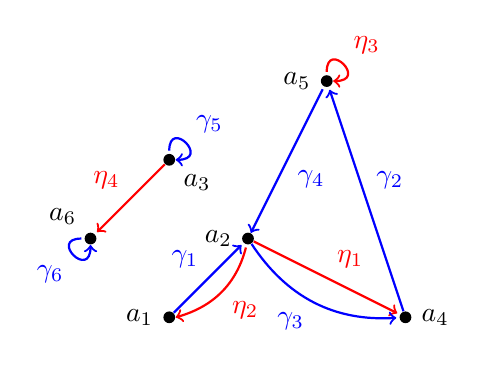
\begin{tikzpicture}
	[object/.style={circle,fill=black,minimum size=1mm,inner sep=1.5pt},
	 bluearrowpre/.style={->,shorten <=1pt,thick,blue},
	 redarrowpre/.style={->,shorten <=1pt,thick,red},
	 bluearrowpost/.style={<-,shorten <=1pt,thick,blue},
	 redarrowpost/.style={<-,shorten <=1pt,thick,red}];
\node[object,label={west:$a_1$}] (a1) at (0,0) {};
\node[object,label={west:$a_2$}] (a2) at (1,1) {}
	edge [bluearrowpost] node[auto,swap] {$\gamma_1$} (a1)
	edge [redarrowpre,bend left] node[auto] {$\eta_2$} (a1.east);
\node[object,label={south east:$a_3$}] (a3) at (0,2) {};
\node[object,label={east:$a_4$}] (a4) at (3,0) {}
	edge [redarrowpost] node[auto,swap] {$\eta_1$} (a2) 
	edge [bluearrowpost,bend left] node[auto] {$\gamma_3$}(a2);
\node[object,label={west:$a_5$}] (a5) at (2,3) {}
	edge [bluearrowpost] node[auto] {$\gamma_2$} (a4)
	edge [bluearrowpre] node[auto] {$\gamma_4$} (a2);
\node[object,label={north west:$a_6$}] (a6) at (-1,1) {}
	edge [redarrowpost] node[auto] {$\eta_4$}(a3);

\draw[bluearrowpre] (a3) to [out=90,in=0,loop,looseness=10] node[auto] {$\gamma_5$} (a3);
\draw[redarrowpre] (a5) to [out=90,in=0,loop,looseness=10] node[auto] {$\eta_3$} (a5);
\draw[bluearrowpre] (a6) to [out=180,in=-90,loop,looseness=10] node[auto,swap] {$\gamma_6$} (a6);
\end{tikzpicture}
\end{center}
Now\marginnote[-4cm]{in the graph shown, composites of various morphisms are omitted, 
for instance ${\color{blue}\gamma_3\gamma_1\gamma_2}$} instead of a word in group 
elements, as in the pushout of groups, we take a \emph{path} in this directed graph, 
alternating between edges that come from $\Gamma$ and edges that come from $H$. For 
instance, we could take
\[
	{\color{blue}\gamma_3}{\color{red}\eta_1}{\color{blue}\gamma_2}{\color{red}(\eta_3)^5}{\color{blue}\gamma_4^{-1}}\qquad\text{or}\qquad 
	{\color{red}\eta_4}{\color{blue}(\gamma_6)^{-3}}{\color{red}\eta_4^{-1}}
\]
from the above graph. The `empty' path consisting just of an identity arrow is also an 
option. However, we haven't yet actually constructed $\Gamma\ast_\Lambda H$, merely what 
we might call $\Gamma \ast_{\Lambda_0}H$,\marginnote{if $\Lambda$ is already trivial in 
this sense, then we are done; this is the analogue of the free product of groups} which 
is the pushout where the groupoid $\Lambda$ is replaced by the trivial groupoid 
$\disc(\Lambda_0)$ with the same objects but only identity arrows. What we need to do is 
add `relations', namely extra equalities between morphisms in $\Gamma 
\ast_{\Lambda_0}H$. What this means is that for each morphism $\lambda$ in $\Lambda$, we 
identify the morphisms ${\color{blue}F(\lambda)}$ and ${\color{red}G(\lambda)}$, or more 
precisely, quotient by the equivalence relation on each hom-set of $\Gamma 
\ast_{\Lambda_0}H$ generated by these identifications. For instance, if in the above 
graph, $\gamma_1=F(\lambda_1)$ and $\eta_1 = G(\lambda_1)$, then we add the equality 
$\gamma_1=\eta_1$. This would have the effect of making
\[
	{\color{blue}\gamma_3}{\color{red}\eta_1}{\color{blue}\gamma_2}{\color{red}(\eta_3)^5}{\color{blue}\gamma_4^{-1}} = 
	{\color{blue}(\gamma_3\gamma_1\gamma_2)}{\color{red}(\eta_3)^5}{\color{blue}\gamma_4^{-1}}	
\]
Concatenation of strings and simplifying is the composition in ${\Gamma\ast_\Lambda H}$.

\begin{ex}
Prove that this construction makes $\Gamma\ast_\Lambda H$ a groupoid.
\end{ex}

If we are interested in merely looking at the group of morphisms from a single object $a_i$ to itself,
which is the case when calculating a fundamental group using the groupoid Seifert--van~Kampen,
then we should look at paths that start and finish at the chosen $a_i$.


\begin{example}

Let us look at an example, arising from an application of Seifert--van~Kampen. Consider 
the circle $S^1$ as sitting in $\CC$, and let $U=S^1\setminus \{-i\}$, $V=S^1\setminus 
\{i\}$. All three of these are path connected, and let us take $A={+1,-1} \subset U\cap 
V$. This choice of data satisfies the hypotheses of SvK. The pushout square
\[
\xymatrix{
	\Pi_1(U\cap V,\{\pm1\}) \ar[r] \ar[d] & \Pi_1(V,\{\pm1\}) \ar[d]\\
	\Pi_1(U,\{\pm1\}) \ar[r] & \Pi_(S^1,\{\pm1\})
}
\]

can be simplified as follows. First, $U \simeq (-2,2) \simeq V$, in a way that preserves 
$A=\{\pm1\}$, so that 
\[
\Pi_1(U,\{\pm1\})  \simeq \mathbf{2} = (-1 \stackrel[\gamma^{-1}]{\gamma}{\leftrightarrows} +1)
\qquad \Pi_1(V,\{\pm1\})  \simeq \mathbf{2} = (-1 \stackrel[\eta]{\eta^{-1}}{\leftrightarrows} +1)
\]
and we have omitted the identity arrows. Here $\gamma$ is a path that runs anticlockwise around $S^1$ from $+1$ to $-1$, and $\eta$ is a path that runs anticlockwise from $-1$ to $+1$.
Second, $\Pi(U\cap V,\{\pm1\}) = \disc(\{+1,-1\})$, so
we are in the easier situation as first outlined above, where no additional quotient needs
to be done. The pushout then looks like
\[
\xymatrix{
*+[F]{-1\phantom{\leftrightarrows}+1} \ar[r] \ar[d] 
& 
*+[F]{-1 {\color{red}\stackrel[\eta]{\eta^{-1}}{\leftrightarrows}} +1}\ar[d] 
\\
*+[F]{-1 {\color{blue}\stackrel[\gamma^{-1}]{\gamma}{\leftrightarrows}} +1} \ar[r] &
\Pi_1(S^1,\{\pm1\})
}
\]
The graph we need so as to generate $\Pi_1(S^1,\{\pm1\})$ is then
\begin{center}
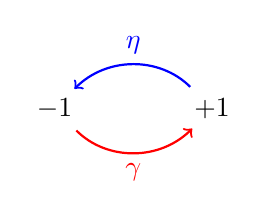
\begin{tikzpicture}
[object/.style={circle,fill=black,minimum size=0.3mm},
	 bluearrow/.style={->,shorten <=1pt,thick,blue},
	 redarrow/.style={->,shorten <=1pt,thick,red}];
\node (plusone) at (0,0) {$-1$};
\node (minusone) at (2,0) {$+1$};

\draw[bluearrow] (minusone) to [out=135,in=45] node[auto,swap] {$\eta$}  (plusone) ;
\draw[redarrow] (plusone) to [out=-45,in=-135] node[auto,swap] {$\gamma$} (minusone) ;

\end{tikzpicture}
\end{center}

Then if we wish to consider paths from $+1$ to itself, the only options are the empty 
path, hence the identity arrow, or $(\eta\gamma)^n$, or $(\gamma^{-1}\eta^{-1})^n = 
(\eta\gamma)^{-n}$. Thus $\pi_1(S^1,+1) \simeq \ZZ$.
\end{example}

\begin{ex}
Prove that this construction of $\Gamma\ast_\Lambda H$ is indeed the pushout in $\Gpd$!
\end{ex}

We will consider one more variant of Seifert--van~Kampen, and this time in brief, 
because the details are similar to other versions. If we would like to compute the 
fundamental group of a join, then it is not quite enough to just consider the free 
product of the fundamental groups: a join does not automatically come with a cover of 
the sort we need for SvK. In what follows, assume: $(X,x)$, $(Y,y)$ are pointed spaces 
such that there exist nhds $x\in U\subseteq X$ and $y\in V\subseteq Y$ that are 
contractible\marginnote{this implies $U\vee V$ is contractible to the basepoint 
$\ast=[x]=[y]$} to $x$ and $y$ respectively, with the contraction fixing the basepoint. 
Then $\{X\vee V, U\vee Y\}$ is a cover of $X\vee Y$ by nhds. We have retractions $X\vee 
V \to X$ and $U\vee Y \to Y$ that preserve the basepoints and which are also homotopy 
equivalences. Thus $\pi_1(X\vee V,\ast)\simeq \pi_1(X,x)$ and $\pi_1(U\vee Y,\ast) 
\simeq \pi_1(Y,y)$, and $\pi_1(U\vee V,\ast)$ is trivial. If we apply the 
Seifert--van~Kampen theorem to the pushout square
\[
\xymatrix{
	(U\vee V,\ast) \ar[r] \ar[d] & (U\vee Y,\ast) \ar[d] \\
	(X\vee V,\ast) \ar[r] & (X\vee Y,\ast)
}
\]
then we get a pushout square of groups
\[
\xymatrix{
	1 \ar[r] \ar[d] & \pi_1(Y,y) \ar[d] \\
	\pi_1(X,x) \ar[r] & \pi_1(X\vee Y,\ast)
}
\]
or in other words, 
\[
	\pi_1(X\vee Y,\ast) = \pi_1(X,x) \ast \pi_1(Y,y).
\]
This generalises the fact that $\pi_1(S^1\vee S^1,\ast) = F_2 = \ZZ\ast \ZZ$ to more 
general spaces.

\begin{fact}
Given any presentation $G=\langle g_1,\ldots,g_m\mid R_1=e,\ldots,R_n=e\rangle$ there is a space
$X$ arising as a pushout\marginnote{$\bigvee_{j=1}^mS^1 = \underbrace{S^1\vee \ldots \vee S^1}_{m\text{ times}}$}
\[
\xymatrixnocompile{
	\bigsqcup_{i=1}^n S^1 \ar[r] \ar[d]_{\langle f_1,\ldots,f_n\rangle} 
		& \bigsqcup_{i=1}^n D^2 \ar[d]\\
	\bigvee_{j=1}^m S^1 \ar[r] & X
}
\]
where $f_i(1)=R_i$, with the property that $\pi_1(X,\ast)\simeq G$. This space is in some 
sense 2-dimensional as it is gotten by gluing together 2d discs, and sometimes a manifold, though not always.

Even better, for \emph{any} group $G$ with any presentation, there is an appropriate pushout
\[
\xymatrixnocompile{
	\bigsqcup_{\beta \in J} S^1 \ar[r] \ar[d]_{\langle f_\beta\rangle} 
		& \bigsqcup_{\beta \in J} D^2 \ar[d]\\
	\bigvee_{\alpha\in I} S^1 \ar[r] & X
}
\]
with the property that $\pi_1(X,\ast) \simeq G$. One has to be careful with the 
topology, and we haven't defined infinite joins,\marginnote{the coutable join 
$\bigvee_{n\in \NN}S^1$ may seem like the Hawaiian earring, but it is in fact not 
compact, and \emph{is} slsc, so they cannot be homeomorphic} but it does work out that 
$\pi_1(\bigvee_{\alpha\in I}S^1,\ast) \simeq F_I$, the free group on the set $I$.
\end{fact}

\begin{example}
An oriented compact Riemann surface $\Sigma_g$ of genus $g\geq 1$ is an example of a 
 surface gotten by a construction as in the Fact above, and even better: it only 
 requires one copy of $D^2$. For genus $g$, it requires doing a pushout of the form
\[
\xymatrixnocompile{
	S^1 \ar[d] \ar[r] & D^2 \ar[d] \\
	\bigvee_{i=1}^{2g} S^1 \ar[r] & \Sigma_g
}
\]
An alternative way to build this pushout is to consider a $4g$-gon,\marginnote{Insert 
octagon picture for case $g=2$ here} and selectively identify edges in pairs (recovering the 
$2g$ circles as in the pushout). The pattern of identifications is exactly that which 
gives rise to the one-relator group after Example~\ref{eg:one-relator_group}, since the 
\emph{attaching map} $S^1 \to \bigvee_{i=1}^{2g} S^1$ in the preceeding pushout is given 
by $\prod_{i=1}^g[a_i,b_i]$, for $a_i$ and $b_i$ the generators of the $2i-1$th and 
$2i$th copy of $S^1$ respectively.
\end{example}

\section{Classifying covering spaces}

Recall\lecturenum{14}
 that for a covering space $Z\xrightarrow{\pi} X$ we get a representation 
\begin{align*}
\rho_Z\colon \Pi_1(X)& \longrightarrow \Set \\
x & \mapsto Z_x\\
[\gamma\colon x\rightsquigarrow y] & \mapsto \left(\gamma_*\colon Z_x\xrightarrow{\simeq} Z_y\right)
\end{align*}

of the fundamental\marginnote{$\xymatrix{Z_1 \ar[rr]^f \ar[dr]_{\pi_1} && Z_2 
\ar[dl]^{\pi_2}\\ & X}$} groupoid of $X$. Given a pair of covering spaces $Z_1,Z_2\to X$ 
and a map between them in $\Cov_X$, how are the representations $\rho_{Z_1}$ and 
$\rho_{Z_2}$ related? Since the triangle at right commutes, we get for each $x\in X$ a 
function between the corresponding fibres, $f\big|_x \colon (Z_1)_x \to (Z_2)_x$. Notice 
that this is a function $\rho_{Z_1}(x) \to \rho_{Z_2}(x)$ for each object of $\Pi_1(X)$. 
Given a path $\gamma\colon x\rightsquigarrow y$ in $X$ and $z\in (Z_1)_x$, we have the 
unique lift to $Z_1$ starting at $z$, namely $\widetilde{\gamma_z}^1\colon 
z\rightsquigarrow \gamma_*(z)$. By composing with $f$, we get a path $f\circ 
\widetilde{\gamma_z}^1\colon I \to Z_2$ from $f(z)$ to $f(\gamma_*(z))$. But by 
uniqueness of lifts of paths, this is the lift of $\gamma$ 
to $Z_2$ starting at $f(z)$, which is a path from $f(z) \rightsquigarrow \gamma_*(f(z))$.
We thus get $f(\gamma_*(z)) = \gamma_*(f(z))$ for every $z\in (Z_1)_x$, implying that the
following square commutes:
\[
\xymatrix{
	(Z_1)_x \ar[r]^{\gamma_*}  \ar[d]_{f\big|_x} &  (Z_1)_y \ar[d]^{f\big|_y} \\
	(Z_2)_x \ar[r]_{\gamma_*} & (Z_2)_y
}
\]
Or, in other words, the functions $f\big|_x$ define a natural transformation 
$\rho_{Z_1}\Rightarrow \rho_{Z_2}$. This leads us to

\begin{prop}
The mapping $(Z \xrightarrow{\pi} X) \mapsto \rho_Z$\marginnote{Recall that the category $[\cC,\Set]$ has as objects the functors $\cC\to \Set$, and as morphisms the natural transformations} define a functor
\[
	\Cov_X \longrightarrow [\Pi_1(X),\Set].
\]
\end{prop}

\begin{proof}
The natural transformation $\rho_Z \Rightarrow \rho_Z$ associated to the identity map 
$Z\to Z$ has a components the identity functions $Z_x\to Z_x$, hence is the identity 
natural transformation. Also, using uniqueness of path lifting one can show that given 
two composable maps of covering spaces, we get functoriality.
\end{proof}

\begin{example}

Regard $S^1\subset \CC$. Recall the covering spaces $\exp(2\pi i(-))\colon \RR \to S^1$ and $S^1 
\xrightarrow{(-)^n} S^1$, for $n>1$. There is a map of covering spaces
\[
\xymatrix{
\RR \ar[rr]^{\exp(2\pi i(-)/n)} \ar[dr]_{\exp(2\pi i(-))} && S^1 \ar[dl]^{(-)^n} \\
& S^1
}
\]
The fibres of $\RR \to S^1$ are isomorphic to $\ZZ$, and indeed the fibre over $1\in 
S^1$ \emph{is} $\ZZ$. The fibre over $1$ of $S^1 \to S^1$ is $\ZZ/n$, and we get the induced map
\begin{align*}
	\ZZ&\to \ZZ/n\\
	k & \mapsto k \pmod{n}
\end{align*}

Now note that if we focus on the point $1\in S^1$, then a morphism in $\Pi_1(S^1)$ from 
$1$ to itself is the homotopy class of some loop, which can identify with an integer 
under $\pi_1(S^1,1) \simeq \ZZ$. Then the representation associated to $\RR\to S^1$ is
\begin{align*}
\rho_\RR\colon \Pi_1(S^1)& \longrightarrow \Aut(\ZZ) \\
m &\mapsto (k\mapsto k+m)
\end{align*}
whereas the representation associated to $(-)^n\colon S^1\to S^1$ is
\begin{align*}
\rho_n\colon \Pi_1(S^1)& \longrightarrow \Aut(\ZZ/n)\simeq S_n \\
m &\mapsto (k\mapsto k+m \pmod{n})
\end{align*}
The map $\ZZ\to \ZZ/n$ is clearly equivariant for the shift action of $\ZZ$ as shown, as 
a special case of the naturality of the map $\ZZ\to \ZZ/n$.
\end{example}


\begin{q}
What representations $\Pi_1(X) \to \Set$ can arise as $\rho_Z$ for some covering space $Z\to X$?
\end{q}

Recall that it is obvious that every set is the set of connected components of some 
space, and while we didn't go into details, the construction of a space $X$ with 
$\pi_1(X,\pt)\simeq G$ for any given $G$ is a relatively uncomplicated pushout. However, 
given a representation $\Pi_1(X) \to \Set$, it is not immediately obvious how to build a 
covering space giving rise to it. Indeed, all the covering spaces we have seen so far 
are either natural examples we happen to have seen, or special toy cases chosen to 
illustrate some small aspect of the fundamental groupoid of a particularly simple space. 
We are going to look at doing some reductions to simpler cases, on both sides (the 
topological, $\Cov_X$ and the algebraic, $[\Pi_1(X),\Set]$) to make the task easier.

First, since we have the blanket assumption that out spaces are slpc, we can consider 
finding a section to the continuous map $X\to [\pt,X]$, namely $A\colon [\pt,X] \to X$, 
that picks out one point $a_i$ per path component $X_i \subseteq X$. We have the full 
subgroupoid inclusion $\Pi_1(X,A) \into \Pi_1(X)$ that is additionally an 
equivalence.\marginnote{by an argument as in the solutions for assignment 2, question 7} 
Let us denote by $I$ the set $[\pt,X]$ in what follows.

\begin{lemma}
If $i\colon \cC\into \cD$ is a full subcategory inclusion that is also an equivalence, then 
the restriction map
\begin{align*}
[\cD,\Set]& \xrightarrow{i^*} [\cC,\Set]\\
F & \mapsto F\circ i
\end{align*}
is an equivalence of categories.
\end{lemma}

\begin{proof}
Exercise.
\end{proof}

Now notice also that $\Pi_1(X,A) = \Pi_1(\bigsqcup_{i\in I}X_i,\bigsqcup_{i\in I}\{a_i\}) \simeq \bigsqcup_{i\in I} \mathbb{B}\pi_1(X_i,a_i)$

\begin{lemma}
For any family of categories $(\cC_i)_{i\in I}$ we have an isomorphism\marginnote{An object of a product of family of cateories is a tuple of objects, one from each of the categories, and similar with the morphisms}
\[
	[\bigsqcup_{i\in I} \cC_i,\Set] \xrightarrow{\simeq} \prod_{i\in I}[\cC_i,\Set]. 
\]
\end{lemma}

\begin{proof}
Exercise.
\end{proof}

Given a group $G$, we can define the category $G\Set$ which has as objects sets $S$ 
equipped with a $G$-action, $G\to \Aut(S)$, and with morphisms \emph{equivariant} 
functions.\marginnote{An equivariant function $f\colon S\to T$ satisfies $f(g\cdot p) = 
g\cdot f(p)$ for all $p\in S$} Note that for any groupoid $\Gamma$ and representation 
$\rho\colon \Gamma \to \Set$, for each object $x\in \Gamma_0$ there is a permutation 
representation $\Gamma(x,x) \to \Aut(\rho(x))$. To any natural transformation 
$\rho\Rightarrow \rho'$ between representations, there is an equivariant map between 
$\Gamma(x,x)$-sets, and this is functorial.

\begin{lemma}
The functor just described gives an isomorphism $[\mathbb{B}G,\Set] \xrightarrow{\simeq} G\Set$ of categories
\end{lemma}

We can put all of these lemmas together and get an equivalence of categories
\[
[\Pi_1(X),\Set] \to [\Pi_1(X,A),\Set] \simeq \prod_{i\in I}[\mathbb{B}\pi_1(X_i,a_i),\Set]
\simeq \prod_{i\in I}\pi_1(X_i,a_i)\Set.
\]
We can compose this with the original functor we were looking at, from covering spaces to representations, to get
\begin{align}
	\Cov_X & \to \prod_{i\in I}\pi_1(X_i,a_i)\Set \label{eq:fibre_functor}\\
	(Z\to X) & \mapsto (\rho_i\colon \pi_1(X_i,a_i) \to Z_{a_i})_{i\in I} \nonumber
\end{align}
where now the codomain is much more tractable. Further, the objects in categories of the 
form $G\Set$ are not unreasonable: we can break them down into smaller parts. Each 
object $\rho\colon G\to \Aut(S)$ in $G\Set$ isomorphic to one of a particularly nice 
form, namely $S\simeq \bigsqcup_{j\in S/G} G/\mathrm{Stab}(p_j)$, where the points 
$p_j\in S$ are chosen so that there is one in each orbit of the $G$-action.

\begin{rem}
From now on, we will consider only spaces that are slsc, since this will ultimately be 
the case in the classification theorem, and also because $X$ slsc implies that for every 
covering space $Z\to X$, the space $Z$ is locally path connected, so that path 
components and components agree.
\end{rem}

\lecturenum{15}
\begin{lemma}
For a space $X = \bigsqcup_{i\in I} X_i$, there is an equivalence of categories $\Cov_X \simeq \prod_{i\in I} \Cov_{X_i}$.
\end{lemma}

\begin{proof}
A covering space $Z\to \bigsqcup_{i\in I} X_i$ gives covering spaces $Z_{X_j}:=\mathrm{in}_j^*X$ for each $j\in I$, where recall the inclusion maps $\mathrm{in}_j\colon X_j \to \bigsqcup_{i\in I} X_i$. We also get, from a map of covering space $Z\to Z'$ over $X$, a map $Z_{X_j} \to Z'_{X_j}$ of covering spaces over $X_j$, for each $j$. This gives a functor $\Cov_X \to \prod_{i\in I} \Cov_{X_i}$.

Conversely, given a covering space $Z_i \to X_i$ for each $i\in I$, we get a covering space $\bigsqcup_{i\in I} Z_i \to \bigsqcup_{i\in I} X_i$, and for maps $Z_i \to Z'_i$ of covering spaces over $X_i$, there is a map $\bigsqcup_{i\in I} Z_i \to \bigsqcup_{i\in I} Z'_i$ of covering spaces over $\bigsqcup_{i\in I}X_i$. This gives a functor $\prod_{i\in I} \Cov_{X_i} \to \Cov_X$, and these two functors are an equivalence of categories.
\end{proof}

The functor in (\ref{eq:fibre_functor}) then factorises as the composite
\begin{align*}
	\Cov_X & \xrightarrow{\simeq} \prod_{i\in I} \Cov_{X_i} \longrightarrow \prod_{i\in I}\pi_1(X_i,a_i)\Set\\
	\raisebox{4ex}{\xymatrix{Z\ar[d]\\X}} & \mapsto 
	\raisebox{4ex}{\xymatrix{Z_{X_i}\ar[d]\\X_i} } \mapsto 
	\left(\rho_i\colon \pi_1(X_i,a_i) \to \Aut(Z_{a_i}) \right)
\end{align*}
In particular, if we understand each $\Cov_{X_i} \to\pi_1(X_i,a_i)\Set$, then we are done. 

So, we will consider from now on the case of a connected, slsc space $X$ with chosen $x_0\in X$, and the functor $\Cov_{X} \to\pi_1(X,x_0)\Set$. 

Since $X$ is slsc, it is locally path connected, and the local trivialisation of any covering space $Z\to X$ shows that $Z$ is also locally path connected.\marginnote{there is a small subtlety here, in that we really require a basis of nhds that are path connected, I will expand on this point if pushed, but it is a technicality that can be ignored for our purposes} We can then write $Z = \bigsqcup_{\alpha \in I} Z_\alpha \to X$, where each $Z_\alpha \to X$ is a (path) connected covering space.\marginnote{Exercise!}

\begin{example}
Take $X=S^1$. Recall that we have various covering spaces: $S^1\times F\simeq \bigsqcup_{F} S^1\to S^1$ for discrete spaces $F$; the exponential map $\RR \to S^1$; the various $S^1 \xrightarrow{(-)^n} S^1$ with $n>1$, where we shall write $S^1_n$ for the total space of this covering space. Then we can form a covering space
\[
	S^1\times F \sqcup \bigsqcup \RR \sqcup \bigsqcup S^1_2 \sqcup \bigsqcup S^1_3\sqcup \ldots \to S^1.
\]
It remains to be seen, however, if there are any covering spaces not of this form.
\end{example}

Recall from lecture 6 (on page~\pageref{eq:fibre_quotient_of_loops}) that given a covering space $Z\to X$, there is a surjective map
\[
	\Omega_{x_0} X \times\{z_\alpha\mid \alpha \in I\} \to Z_{x_0}, \qquad z_\alpha \in Z_{x_0}\cap Z_\alpha,
\]
hence a surjective map \[
	\pi_1(X,x_0) \times \{z_\alpha\mid \alpha \in I\} \simeq \bigsqcup_{\alpha\in I}\pi_1(X,x_0) \times  \{z_\alpha\} \to Z_{x_0} = \bigsqcup_{\alpha\in I} Z_{x_0}\cap Z_\alpha
\]
\begin{lemma}
Given a covering space $Z\to X$ with $x_0\in X$, then $Z_{x_0} =\bigsqcup_{\alpha\in I} Z_{x_0}\cap Z_\alpha\simeq \bigsqcup_{\alpha\in I} \pi_1(X,x_0)/\pi_1(Z_\alpha,z_\alpha)$ as $\pi_1(X,x_0)$-sets, for any choice of $z_\alpha\in Z_{x_0}\cap Z_\alpha$.
\end{lemma}

\begin{proof}
It is enough to show that the orbits of the $\pi_1(X,x_0)$-action are the sets $Z_{x_0}\cap Z_\alpha$, because then the general description of sets with transitive action takes over. Given $z\in Z_{x_0}\cap Z_\alpha$, there is a path $\gamma\colon z_\alpha \rightsquigarrow z$, and hence a loop $\pi\circ\gamma$ at $x_0$. This loop acts on $Z_{x_0}$, with $(\pi\circ \gamma)_*(z_\alpha)=z$. Hence $Z_{x_0}\cap Z_\alpha$ is contained in the orbit containing $z_\alpha$. Conversely, given any $z\in Z_{x_0}$ and a loop $\eta$ at $x_0$ such that $\eta_*(z_\alpha) = z$, then there is a lift $\widetilde{\eta}\colon z_\alpha \rightsquigarrow z$ of $\eta$, so that $z\in Z_\alpha$. Thus the orbit of $z_\alpha$ is contained in $Z_{x_0}\cap Z_\alpha$, and we are done.
\end{proof}

As a result, our functor $\Cov_X \to \pi_1(X,x_0)\Set$ preserves disjoint unions: it sends the covering space $\bigsqcup_{\alpha \in I} Z_\alpha\to X$ to the disjoint union of sets with a permutation representation $\bigsqcup_{\alpha\in I} Z_{x_0}\cap Z_\alpha$.

\begin{rem}
Given a group $G$ and a $G$-set $S$, such that $S=\bigsqcup_{\alpha\in I} S_\alpha$ is the partition into orbits of the action, then the representation $\rho \colon G\to \Aut(\bigsqcup S_{\alpha\in I})$ factors through the subgroup $\prod_{\alpha\in I} \Aut(S_i) < \Aut(\bigsqcup S_{\alpha\in I})$, hence $\rho = (\rho_\alpha)_{\alpha\in I}$, for $\rho_\alpha\colon G\to \Aut(S_\alpha)$ a transitive $G$-action.
\end{rem}

Recall what our original question was: what representations $\Pi_1(X)\to \Set$ arise from covering spaces of $X$ via the functor $\Cov_X \to [\Pi_1(X),\Set]$? We have now reduced this to the simpler aim of starting with a permutation representation of a fundamental group, and can reduce the input data even more. Inside $\Cov_X$ (for connected $X$) is the full subcategory $\Cov_X^\mathrm{conn}$ of \emph{connected} covering spaces, and inside $\pi_1(X,x_0)\Set$ is the full subcategory $\pi_1(X,x_0)\Set^\mathrm{tr}$ of sets with a \emph{transitive} action. Moreover, in both of these cases, arbitrary objects in $\Cov$ and $\pi_1(X,x_0)\Set$ can be gotten by disjoint union of objects in the respective subcategories. Thus it is sufficient to ask if we can get any transitive $\pi_1(X,x_0)$-set from some connected covering space of $X$. That is, we want to know what is the image of the functor
\[
	\Cov_X^\mathrm{conn} \longrightarrow  \pi_1(X,x_0)\Set^\mathrm{tr}.
\]

Note that in the category of transitive $G$-sets, every object $S$ with a point $p\in S$ is the quotient of the underlying set of $G$ equipped with the action by multiplication, via the map 
\begin{align*}
G& \to S \simeq G/\mathrm{Stab}(p)\\
g & \mapsto g\cdot p
\end{align*}
and the $G$-action on $G$ is free and transitive. More generally, given any $G$-set $T$ with a free and transitive action, there is a surjective equivariant map $T\to S$ displaying $S$ as a quotient of $T$.

\begin{example}
Given a simply-connected covering space $Z\to X$ and $x_0\in X$, the fibre $Z_{x_0}$ is a free and transitive $\pi_1(X,x_0)$-set.
\end{example}

Recall also that for a general path connected covering space $Z\to X$, $Z_{x_0} \simeq \pi_1(X,X_0)/\pi_1(Z,z)$ for any $z\in Z_{x_0}$. If we start with a pointed covering space, then we don't have to choose a point, and every connected covering space of a pointed space can be gotten by forgetting the point from some pointed covering space.
So we have the final form of the question

\begin{q}
Given a subgroup $H< \pi_1(X,x_0)$, is there a pointed covering space $(Z,z_0)\to (X,x_0)$ such that $\pi_1(Z,z_0) = H$ as subgroups of $\pi_1(X,x_0)$?\marginnote{Recall from assignment 2, where from a simply-connected space $Y$ with free $G$-action, we got a covering space $Y\to Y/G$ with $\pi_1(Y/G,\ast)\simeq G$}
\end{q}


Recall\lecturenum{16} that for a simply-connected covering space $Z^{(1)} \to X$ the fibre over $x_0$ is isomorphic to $\pi_1(X,x_0)$, and that our ultimate aim is to get a covering space with fibre isomorphic to $\pi_1(X,x_0)/H$. So one way to approach this is to see if there is a way to make sense of making a covering space by taking the quotient of some simply-connected covering space ``fibre by fibre''. It isn't possible to do this piecemeal, so we need to do this for all fibres at once.

\begin{definition}
Let $p\colon Y\to X$ be a map of spaces, $G$ a group acting on $Y$. We say the action is \emph{fibrewise} if $p(g\cdot y) = p(y)$ for all $y \in Y,g\in G$.
\end{definition}

It follows from the definition\marginnote{there is a commutative triangle $\xymatrix{Y \ar[d] \ar[r] & Y/G \ar[dl]\\ X}$} that there is map $Y/G \to X$, and the fibre of this map over $x$ is $p^{-1}(x)/G$.

\begin{prop}
Let $Z\xrightarrow{\pi} X$ be a covering space, and let $G$ act fibrewise on $Z$. Then $Z/G\to X$ is a covering space and $Z\to Z/G$ is a map of covering spaces.
\end{prop}

\begin{proof}
First notice that since the action of $G$ is fibrewise, the orbits of $G$ are subspaces of discrete spaces, and hence are discrete.

For $U\subseteq X$, we get an action of $G$ on $Z_U \subseteq Z$, also fibrewise for the restriction $Z_U \to U$ of $\pi$. If we take $U$ small enough nhd around $x\in X$ then $Z_U \simeq Z_x \times U$, and moreover this homeomorphism is $G$-equivariant and respects the maps to $U$. We thus get a homeomorphism $(Z_U)/G \simeq U \times (Z_x/G)$. Then, from the question in assignment 4, $(Z/G)_U$ is homeomorphic to $(Z_U)/G$ over $U$, so there is a homeomorphism $(Z/G)_U \simeq U \times (Z_x/G)$ over $U$, and hence $Z/G \to X$ is a covering space with fibre $Z_x/G$. The quotient map $Z \to Z/G$ respects the maps to $X$ by construction, so is a map of covering spaces.
\end{proof}

Thus if $Z^{(1)} \to X$ is a simply-connected covering space and $H< \pi_1(X,x_0)$ acts fibrewise on $Z^{(1)}$, we get a covering space $Z^{(1)}/H \to X$ with fibre $\pi_1(X,x_0)/H$ \emph{as sets}. However, more is true.

\begin{lemma}
Assuming there is a simply-connected covering space $Z^{(1)} \to X$, the morphism $Z^{(1)}_x \to Z^{(1)}_x/H$ is $\pi_1(X,x)$-equvariant.
\end{lemma}

\begin{proof}
Exercise. Uses path lifing and the map $Z^{(1)} \to Z^{(1)}/H$ over $X$.
\end{proof}

We have have two problems:
\begin{enumerate}
\item How do we construct a simply-connected covering space of $X$? Or how do we know one exists?
\item Given such a thing, and an arbitrary subgroup $H<\pi_1(X,x_0)$, how do we construct a fibrewise $H$-action?
\end{enumerate}


We can reduce the second problem to the case of finding a fibrewise $\pi_1(X,x_0)$-action, because then by restriction, any subgroup will also act fibrewise. As it turns out, the construction that will address the first point will also automatically come with the required fibrewise action of the fundamental group.

\begin{construction}
Fix a pointed space $(X,x_0)$. Consider the quotient space $X^{(1)} := P_{x_0}X/\sim$ where $\gamma_1\sim \gamma_2$ if $\gamma_1(1)=\gamma_2(1)$ and $[\gamma_1]=[\gamma_2]$ in $\Pi_1(X)$. From the definition of the equivalence relation and the quotient topology, we get a continuous pointed map $X^{(1)} \to X$ and a commutative triangle\marginnote{we will denote the class of the constant path also by $c_{x_0}$ to de-clutter the notation}
\[
	\xymatrix{
	(P_{x_0},c_{x_0}) \ar[rr] \ar[dr] && (X^{(1)},c_{x_0}) \ar[dl]\\
	& (X,x_0)
	}
\]
\end{construction}

Thus one can see this as giving a topology to a subset of the morphisms of $\Pi_1(X)$.

\begin{prop}
For $X$ semilocally simply-connected, $(X^{(1)},c_{x_0}) \to (X,x_0)$ is a simply-connected covering space, and $\pi_1(X,x_0)$ acts by concatenation as in $\Pi_1(X)$
\end{prop}

\begin{proof}
Notice first that the fibre $X^{(1)}_x$ of $X^{(1)} \to X$ over $x\in X$ is $\Pi_1(X)(x_0,x) \simeq P_{x_0}^xX/\sim$, and moreover, since $X$ is slsc, $P_{x_0}^xX$ is slpc, and hence $X^{(1)}_x=[\pt,P_{x_0}^xX]=\pi_0(P_{x_0}^xX)$ is discrete. Thus $X^{(1)} \to X$ has discrete fibres.

Now fix $x\in X$. Since $X$ is slsc, there is a nhd $U\ni x$ such that for every $x'\in U$ there is a path $\eta_{x'}\colon x\rightsquigarrow x'$ (in $U$) such that for any other path $\eta\colon x \rightsquigarrow x'$ in $U$, $[\eta_{x'}]=[\eta]$ in $\Pi_1(X)$. Consider $X^{(1)}_U = \{[x_0\rightsquigarrow x']\mid x'\in U\}$.

\textbf{Claim:} There is a homeomorphism 
\begin{align*}
U\times X^{(1)}_x & \xrightarrow{\simeq} X^{(1)}_U \\
(x',[x_0 \stackrel{\gamma}{\rightsquigarrow} x]) \mapsto [x_0 \stackrel{\gamma}{\rightsquigarrow} x \stackrel{\eta_{x'}}{\rightsquigarrow} x']
\end{align*}
over $U$. We can prove this is a bijection without too much difficulty, as follows. 
\begin{itemize}
\item Injective: If $[x_0 \stackrel{\gamma}{\rightsquigarrow} x \stackrel{\eta_{x'}}{\rightsquigarrow} x'] = [x_0 \stackrel{\gamma'}{\rightsquigarrow} x \stackrel{\eta_{x'}}{\rightsquigarrow} x']$, then we can concatenate with $-\eta_{x'}$ and the result is that $[\gamma] = [\gamma']$.
\item Surjective: Suppose I have $[x_0 \stackrel{\gamma}{\rightsquigarrow} x'] in X^{(1)}_U$. Then $[\gamma] = [\gamma][\eta_{x'}]^{-1}[\eta_{x'}]$.
\end{itemize}

For now, for the proof that this is a homeomorphism, see pages 64--65 of Hatcher, in the section ``The Classification of Covering Spaces''.\marginnote{I will fill in the details here later}

Thus we have a local trivialisation, and hence a covering space.

We can see that $X^{(1)}$ is path connected by observing that it is the quotient of the path connected space $P_{x_0} X$\marginnote{there is a path from $c_{x_0}$ to any $\gamma\colon x_0\rightsquigarrow x$, defined by $s\mapsto (t\mapsto \gamma(st))$}, hence there is a surjective map $P_{x_0}X \to X^{(1)}$. 

There is a fibrewise action of $\pi_1(X,x_0)$ on $X^{(1)}$ by $([x_0 \stackrel{\omega}{\rightsquigarrow} x_0],[x_0 \stackrel{\gamma}{\rightsquigarrow} x]) \mapsto [x_0 \stackrel{\omega}{\rightsquigarrow} x_0 \stackrel{\gamma}{\rightsquigarrow} x]$. This is continuous because it is induced from the continuous concatenation $\Omega_{x_0}\times P_{x_0}X \to P_{x_0}X$, and the axioms for an action hold from the associativity of composition in $\Pi_1(X)$. Note especially that the $\pi_1(X,x_0)$-action is \emph{free}, so that the stabiliser subgroups are all trivial.

Finally, since the fibre of $X^{(1)}$ at $x_0$ is the quotient of $\pi_1(X,x_0)$ by the stabiliser subgroup by the $\pi_1(X,x_0)$-action, and this stabiliser subgroup is $\pi_1(X^{(1)},c_{x_0})$, we have that $\pi_1(X^{(1)},c_{x_0})$ is trivial. Hence $X^{(1)}$ is simply-connected.
\end{proof}

As a result, given any subgroup $H < \pi_1(X,x_0)$, we can define the connected covering space $X^{(1)}/H \to X$, which is a pointed covering space with $\pi_1(X^{(1)},\ast) = H$. Working backwards through the reasoning above, we can get \emph{any} set with $\pi_1(X,x_0)$-action, up to isomorphism, as the fibre of some covering space of $(X,x)$. And then, if $X$ has multiple connected components, we can the take the disjoint union of covering spaces of each component to get a representation of the whole fundamental groupoid. Thus we have proved

\begin{prop}
For an slsc space $X$ the functor
\[
	\Cov_X \to [\Pi_1(X),\Set]
\]
is essentially surjective: every representation $\Pi_1(X) \to \Set$ is isomorphic to one coming from a covering space.
\end{prop}

We\lecturenum{17} can say still more:

\begin{lemma}
Let $Z\xrightarrow{\pi} X$ be a covering space, $Y$ path connected and $p\colon Y\to X$ be some map. Suppose we have maps $f,g\colon Y\to X$ such that $f\circ \pi = p = g\circ \pi$. Then if $f(y_0) = g(y_0)$ for some $y_0\in Y$, we have $f=g$. 
\end{lemma}

\begin{proof}
Take $y\in Y$ arbitrary, and let $\gamma\colon y_0 \rightsquigarrow y$ be a path. Then $f\circ \gamma$ and $g\circ \gamma$ are both lifts of the path $p\circ \gamma\colon I \to X$. And since $f(\gamma(0)) = f(y_0) = g(y_0) = g(\gamma(y_0))$, we must have $f(y) = f(\gamma(1)) = g(\gamma(1)) = g(y)$. 
\end{proof}

This applies in particular, if $Y$ is another covering space of $X$.

\begin{corollary}
The functor $\Cov_{X} \to [\Pi_1(X),\Set]$ is faithful.
\end{corollary}

\begin{proof}
We can reduce to the case of $X$ connected, and can choose a basepoint $x_0\in X$ to get a functor $\Cov_X \to [\Pi_1(X),\Set] \to \pi_1(X,x_0)\Set$. This functor will be faithful if and only if the original functor is (after the reduction to $X$ connected.) Now suppose we have two covering spaces $Z_i \xrightarrow{\pi_i} X$ ($i=1,2$) and a pair of maps $f,g\colon Z_1 \to Z_2$ between them (over $X$). Then if $f\big|_x =g\big|_x\colon (Z_1)_{x_0} \to (Z_2)_{x_0}$, in particular for each path component of $Z_1$, there is a point $z$ such that $f(z) = f\big|_x(z) =g\big|_x(z) = g(z)$, so that $f$ and $g$ coincide on each path component, and hence agree everywhere.
\end{proof}

In fact, we have the following landmark result:

\begin{theorem}
For slsc $X$, $\Cov_X\to [\Pi_1(X),\Set]$ is an equivalence of categories.
\end{theorem}

The proof reduces to connected and pointed $X$, then shows that given $(Z_1)_x \to (Z_2)_x$ a map of $\pi_1(X,x)$-sets, there is a map $Z_1 \to Z_2$ between covering spaces that induces it. This shows that the functor is full, hence together with the previous results, that it is an equivalence.

\section{Higher homotopy groups}

So far, we have invariants $\pi_0$, $[\pt,-]$\marginnote{treat it as a fluke of low dimensions that there are two invariants that aim to capture what is meant by ``components'' of a space} and $\pi_1$ of a space. Notice that $\pi_1 = [(S^1,1),-]_*$, and in fact for pointed spaces, $[\pt,-] = [(S^0,1),-]_*$, since $S^0 = \{1,-1\}$, and a pointed map $(S^0,1) \to (X,x)$ is specified completely by where it sends $-1$. This leads naturally to the question of what should $\pi_n$ be?

\begin{definition}
Given a pointed space $(X,x)$, define the \emph{$n^{th}$ homotopy group of $X$ based at $x$} to be $[(S^n,1),(X,x)]_*$.
\end{definition}

This is automatically a functor $\Top_* \to \Set$, though we shall soon see we can refine this. It follows quickly from the definition that we have $\pi_n(X\times Y, (x,y)) \simeq \pi_n(X,x)\times \pi_n(Y,y)$.


An important observation is that $S^n$ here can be treated in a number of different ways that all lead to the same definition. Notice\marginnote{For a pair $(Y,A)$, we define the quotient $Y/A$ of $Y$ by the subspace $A$ to be the quotient space $Y/(a_1 \sim a_2, \forall a_1,a_2\in A)$} particularly that $S^n \simeq I^n / \partial I^n \simeq D^n / \partial D^n$. We can take the basepint in $S^n$ to be the image of the collapsed subspace, so that continuous maps of pairs $(I^n,\partial I^n) \to (X,x)$ are in bijection with maps $(S^n,1) \to (X,x)$, and similarly for maps $(D^n,\partial D^n) \to (X,x)$. The relation of homotopy of maps $(Y,A) \to (X,x)$ out of a pair generalises that of a pointed homotopy, and demands that the homotopy $H\colon I \times Y\to X$ maps $I\times A$ to $x$. With this definition of relative homotopy, we have that $[(S^n,1),(X,x)]_* = [(I^n,\partial I^n),(X,x)] = [(D^n,\partial D^n),(X,x)]$.

Further, given a map $f\colon (I^n,\partial I^n) \to (X,x)$, we get a continuous map $I^{n-1} \to \Omega_x X$, and the boundary condition on $f$ implies that $\partial I^{n-1}$ is mapped to the constant loop $c_x$. Thus $\pi_n(X,x) = [(I^n,\partial I^n),(X,x)] \simeq [(I^{n-1},\partial I^{n-1}),(\Omega_x X,c_x)] = \pi_{n-1}(\Omega_x X,c_x)$. Since we know path concatenation is continuous, we have the map $\Omega_x X \times \Omega_x X \to \Omega_x X$. This allows us to define a binary operation
\[
	\pi_n(X,x)\times \pi_n(X,x) \simeq \pi_{n-1}(\Omega_x X,c_x) \times \pi_{n-1}(\Omega_x X,c_x) \simeq \pi_{n-1}(\Omega_x X \times \Omega_x X,(c_x,c_x)) \to \pi_{n-1}(\Omega_x X,c_x)  \simeq \pi_n(X,x)
\]
The up-to-homotopy associativity of the concatenation of loops, together with inverses and identity element up to homotopy, means that $\pi_n(X,x)$ is in fact a group, and so we have a functor $\pi_n\colon \Top_* \to \Grp$. The following  is a famous later abstraction of a result that originally arose when the higher homotopy groups were first defined in 1932 (or so).

\begin{lemma}[Eckmann--Hilton argument]
Let $M$ be a set with two unital binary operations $\circ,\# \colon M \times M \to M$, with units $1_\circ$ and $1_\#$, such that for all $a,b,c,d\in M$, 
\[
	(a \circ b) \# (c\circ d) = (a \# c) \circ (b \# d).
\]
Then $1_\circ = 1_\#$, $a\circ b = a \# b$, $a\# b = b \# a$ and moreover the binary operation is associative, making $M$ an abelian group
\end{lemma}

\begin{proof}
\begin{enumerate}
\item First, $1_\circ = 1_\circ \circ 1_\circ = (1_\circ \# 1_\#) \circ (1_\# \# 1_\circ) = 
(1_\circ \circ 1_\#) \# (1_\# \circ 1_\circ) = 1_\# \# 1_\# = 1_\#$, so that the unit elements agree, and we can just denote $1_\circ = 1_\# =: 1$.

\item Then $a\circ b = (a \# 1) \circ (1 \# b) = (a\circ 1) \# (1\circ b) = a \# b$, so we can write $ab := a\circ b = a \# b$ for the single binary operation.

\item Now $ab = (1a)(b1)=(1b)(a1)=ba$, so that the binary operation is commutative.

\item Finally, $(ab)c = (ab)(1c) = (a1)(bc)=a(bc)$, so that the binary operation is associative, and thus we have an abelian group structure. 
\end{enumerate}
\end{proof}

\begin{example}
If $G$ is a Lie group\marginnote{or even just a topological group} then $\pi_1(G,e)$ is abelian, because we have the concatenation operation, and the operation of pointwise multiplication of loops (which passes down to homotopy classes of loops). The constant loop is the identity element for both of these operations, so we get the first part of the previous lemma for free. The only thing that needs checking is that pointwise multiplication and concatenation distribute as needed for the Eckmann--Hilton argument, but this is not difficult to check.
\end{example}

Now let us go back to our observation that $\Top_*((S^n,1),(X,x)) \simeq \Top_*((S^{n-1},1),(\Omega_x X,c_x))$. We can iterate this, to get  $\Top_*((S^{n-1},1),(\Omega_x X,c_x)) \simeq \Top_*((S^{n-2},1),(\Omega_{c_x}\Omega_x X,c_{c_x}))$. This makes sense because in the definition of the based loop space $\Omega_y Y$, the space $Y$ is arbitrary. Let us write $\Omega^2_x X$ for $\Omega_{c_x}\Omega_x X$, and always assume it has the basepoint $c_{c_x}$. Then there are two continuous concatenation operations
\[
	\Omega^2 X \times \Omega^2 X \to \Omega^2 X,
\]
arising from concatenating in either the first or the second parameter. Given $f_1,f_2\in \Omega^2 X$, that is, functions $I^2\to X$ such that $\partial I^2$ is mapped to $x$, we have
\begin{align*}
(f_1 \#_1 f_2)(s,t) & = \begin{cases}
f_1(2s,t) & \forall t\in I,\ s\in [0,\frac12]\\
f_2(2s-1,t) & \forall t\in I,\ s\in [\frac12,1]
\end{cases}\\
(f_1 \#_2 f_2)(s,t) & = \begin{cases}
f_1(s,2t) & \forall t \in [0,\frac12],\ s\in I\\
f_1(s,2t-1) & \forall t\in [\frac12,1],\ s\in I
\end{cases}
\end{align*}
And, moreover, $(f_1 \#_1 f_2) \#_2 (f_3 \#_1 f_4) = (f_1 \#_2 f_3) \#_1 (f_2 \#_2 f_4)$, where each of these is defined on one quadrant of the $^2$ subdivided into four squares. Thus, from the Eckmann--Hilton argument,

\begin{prop}
The group $\pi_n(X,x)$ is abelian for all $n\geq 2$.
\end{prop}


The\lecturenum{18} assignment 
\begin{align*}
(X,x) & \mapsto \pi_n(X,x)\\
\left(f\colon (X,x) \to (Y,y) \right)& \mapsto \left(f_* \colon \pi_1(X,x) \to \pi_n(Y,y) \right)
\end{align*}
is then a functor $\Top_* \to \Ab$.

\begin{example}
For $S$ a discrete space, $\pi_n(S,*) = 1$, since all $S^n \to S$ are constant maps ($S^n$ is connected!)
\end{example}

\begin{example}
If $X$ is contractible (eg a star-shaped domain in a topological vector space) then $\pi_n(X,x) = 1$
\end{example}

Recall: Given a covering space $Z\to X$ there is an associated representation $\Pi_1(X) \to \Set$. But there is nothing special here about the category $\Set$, we can have other categories, for instance: the category $\Fin$ of finite sets, the category $\Vect$ of vector spaces, the category $\Ab$ of abelian groups, or more generally the category $R\Mod$ of $R$-modules ($R$ here is a given ring).

% \begin{example}
% Given a representation $\Pi_1(X) \to \Set$, we get a representation $\Pi_1 \to \Vect$ by taking composing with the functor $\Set \to \Vect$ that associates to a set the vector space with that basis, and to a function the associated linear map.
% \end{example}

\begin{prop}
Fix the space $X$. The assignment $x\mapsto \pi_n(X,x)$ is the object component of a representation $\Pi_1(X) \to \Ab$.
\end{prop}

\begin{proof}
(Sketch) Given $\gamma\colon [0,1] \to X$, $x\rightsquigarrow y$, and $\alpha\colon (I^n,\partial I^n) \to (X,x)$ representing a class in $\pi_n(X,x)$, we need to construct a class in $\pi_n(X,y)$, in such a way that this gives a group isomorphism $\pi_n(X,x) \xrightarrow{\simeq} \pi_n(X,y)$. For this construction, consider the interval $I = [-\frac12,\frac12]$.
Fix an orientation-preserving homeomorphism $I = [-\frac12,\frac12]\xrightarrow{\simeq} [-\frac14,\frac14]$, and thus a map $i\colon [-\frac14,\frac14]^n  \simeq I^n $. Also fix orientation-preserving $j\colon [\frac14,\frac12]\xrightarrow{\simeq} [0,1]$.  Define $\alpha^\gamma\colon I^n \to X$ to be the piecewise defined function
\[
\alpha^\gamma(\mathbf{x}) = \begin{cases} 
\alpha(i(\mathbf{x})) & \mathbf{x} \in [-\frac14,\frac14]^n\\
\gamma(j(|\mathbf{x}|)) & \mathbf{x} \in [-\frac12,\frac12]^n \setminus [-\frac14,\frac14]^n
\end{cases}
\]
By the pasting lemma this is continuous, as $\alpha(\mathbf{x}) = x$ for all $\mathbf{x} \in \partial I^n$, and $\gamma(0) = x$. Moreover, $\alpha^\gamma(\mathbf{x}) = y$ for all $\mathbf{x} \in \partial I^n$, and so $\alpha^\gamma\colon (I^n,\partial I^n) \to (X,y)$. The homotopy class of $\alpha^\gamma$ is independent of the choice of $\gamma$ and $\alpha$ as representatives for their respective classes in $\Pi_1(X)(x,y)$ and $\pi_n(X,x)$, as we can use homotopies between these and other representatives to create a homotopy between maps $(I^n,\partial I^n) \to (X,y)$. We thus get a function $\pi_n(X,x) \to \pi_n(X,y)$ for each $[\gamma]\in \Pi_1(X)(x,y)$.

As functions between sets, this is functorial by a reparametrisation argument, so that $[\alpha^{\gamma\#\eta}] = [(\alpha^\gamma)^\eta]$, and $[\alpha^{c_x}] = [\alpha]$. The last thing that needs to be checked is that $[\alpha]\mapsto [\alpha^\gamma]$ is a group homomorphism. This is a mildly fiddly, but overall unenlightening argument.\marginnote{there is a proof in Hatcher, \S4.1 on page 341}
\end{proof}

Note that if we consider the case $n=1$, then we have already seen a version of this: given a path $\gamma\colon x\rightsquigarrow y$, there is an isomorphism $\pi_1(X,x) \xrightarrow{\simeq} \pi_1(X,y)$. If we specialise to the case of $x=y$, then $\gamma$ is a loop, and the resulting automorphism $\pi_1(X,x)$ is conjugation by $\gamma$.

\begin{rem}
If $X$ is simply-connected, then we get \emph{canonical} isomorphisms $\pi_n(X,x) \simeq \pi_n(X,y)$ for all pairs of points $x,y\in X$.\marginnote{there is an analogue when we talk about just a simply-connected path component of $X$ and points in it} For this reason, many authors omit basepoints when talking about homotopy groups when it is not important.
\end{rem}

\begin{rem}
Since, for each $n$ we get a representation $\Pi_1(X) \to \Ab$ from the collection of higher homotopy groups $\pi_n(X,x)$, there is a representation $\Pi_1(X) \to \Ab \to \Set$ gotten by composing with the underlying set functor $\Ab \to \Set$. From this we get a covering space of $X$, whose fibre at $x\in X$ is $\pi_n(X,x)$. In fact this covering space `remembers' the fact that each higher homotopy group is actually a group, in that it is a continuously-varying family of groups, not just of sets.
\end{rem}

\begin{lemma}
Given a pair of pointed spaces $(X,x)$ and $(Y,y)$, there is an\marginnote{natural, even} isomorphism $\pi_n(X\times Y,(x,y)) \xrightarrow{\simeq} \pi_n(X,x) \times \pi_n(Y,y)$.
\end{lemma}

Just as we saw that homotopic maps should be considered the same from the point of view of fundamental groups and covering spaces, the same is true for higher homotopy groups

\begin{lemma}
Let $f,g\colon X\to Y$ be homotopic, say via $H\colon I\times X \to Y$. Then there is a commutative triangle
\[
  \xymatrix{
    & \pi_n(Y,f(x)) \ar[dd]^{\simeq}\\
    \pi_n(X,x) \ar[ur]^{f_*} \ar[dr]_{g_*} \\
    & \pi_n(Y,g(x))
  }
\]
\end{lemma}
\begin{proof}
The result follows for the special case of $Y = I\times X$ with $H=\id_{I\times X}$ the homotopy between the inclusion maps $f\colon X\simeq \{0\}\times X \into I \times X$ and $g\colon X\simeq \{1\}\times X \into I \times X$.

\end{proof}

\begin{prop}
If $f\colon X\to Y$ is a homotopy equivalence, then $f_*\colon \pi_n(X,x) \xrightarrow{\simeq} \pi_n(Y,f(x))$ is an isomorphism.
\end{prop}

\begin{proof}
(Idea) Since $f$ is a homotopy equivalence, there is a map $g\colon Y\to X$ such that $g\circ f$ is homotopic to $\id_X$ and $f\circ g$ is homotopic to $\id_Y$. We apply the lemma to these homotopies.
\end{proof}

It is very hard to calculate homotopy groups, and one needs to use all kinds of tricks and sometimes even results from differential topology\marginnote{like Sard's theorem, for example} to even calculate them for relatively simple spaces, like spheres. In fact we don't know all the homotopy groups for \emph{any} sphere $S^n$ with $n>1$. However, once there are a few homotopy groups that we know for `standard' spaces, then we can use the following objects in order to generate relations between homotopy groups of different spaces, and thus calculate more of them. 

\begin{definition}
A \emph{fibre bundle} on a space $X$ is a space $P$ together\marginnote{recall that this means that this diagram commutes: $\xymatrix{\pi^{-1}(U) \ar[rr]^\simeq \ar[dr]_\pi && U\times F \ar[dl]^{\pr_1} \\ & U}$} with a map $\pi\colon P \to X$ such that for every $x\in X$ there is a nhd $U\ni x$ and an isomorphism $\pi^{-1}(U) \xrightarrow{\simeq} U\times F$ over $U$ for some space $F$. In this setting we call $X$ the \emph{base space}, $P$ the \emph{total space} and $F$ the \emph{fibre}.
\end{definition}

It is not obvious, but it follows that for $X$ path connected, we do not need to assume that for every point the space $F$ is some fixed space, as all the fibres $\pi^{-1}(x)$ are automatically (non-canonically) homeomorphic. 

This is a big generalisation of the notion of covering space, in that the space $F$ no longer needs to be discrete.

\begin{example}
Every covering space is a fibre bundle.
\end{example}

\begin{example}
Let $S^3 \subset \CC^2$ be the unit sphere, consisting of pairs of points $(z,w)$ such that $|z|^2 + |w|^2 = 1$. There is a projection map $S^3 \to \mathbb{CP}^1$ sending the point $(z,w)$ to the point of the complex projective line $\mathbf{CP}^1$ with homogeneous coordinates $[z:w]$. By the defining equation, this is well-defined, since we don't have $z$ and $w$ simultaneously vanishing. The preimage of a point $[z:w]$ is homeomorphic to a copy of the unit complex numbers $U(1) \subset \CC$. This is a famous fibre bundle, called the \emph{Hopf bundle}. There are very few fibre bundles whose base space, total space and fibre are all spheres, so this is a somewhat atypical object, but very concrete and a good test case for trying out new ideas.
\end{example}

We need to relate homotopy groups of different spaces not just via the functoriality we already know about, but even homotopy groups in different dimensions.

\begin{definition}
A sequence
\[
  \cdots \to A_{n-1} \xrightarrow{f_{n-1}} A_n \xrightarrow{f_n} A_{n+1} \to \cdots 
\]
of (abelian) groups and homomorphisms is called \emph{exact at $A_n$} if $\ker(f_n) = \im(f_{n-1})$. It is called \emph{exact} if it is exact at $A_n$ for all $n$.
\end{definition}

\begin{example}
A special case is where we have three successive nonzero terms:
\[
  0\to A \xrightarrow{\alpha} B \xrightarrow{\beta} C \to 0
\]
Such an exact sequence is called a \emph{short exact sequence}. It has the properties that: $\alpha$ is injective, $\beta$ is surjective, and $\ker(\beta) = \im(\alpha)$.
\end{example}

An even more trivial-seeming example, that still turns up in practice

\begin{example}
A sequence $0\to A \xrightarrow{\phi} B \to 0$ is exact if and only if $\phi$ is an isomorphism.
\end{example}

\begin{rem}
The definition of exact sequence still makes sense (just!) for pointed sets and functions: given $(A,a) \xrightarrow{f} (B,b) \xrightarrow{g}  (C,c)$ pointed functions, this is exact at $(B,b)$ if $\im(f) = g^{-1}(c)$. The reason we care about this is that if $(X,x)$ is a pointed space $[\pt,X] \simeq [S^0,(X,x)]_*$ is a pointed set.
\end{rem}

Given a fibre bundle $\pi\colon P\to X$, we say it is pointed if we are given $x\in X$ and some $p\in F = \pi^{-1}(F)$.

\begin{theorem}
For a pointed fibre bundle $(P,p) \to (X,x)$, there is an exact sequence
\[
\hspace{-1.5cm}\cdots \to \pi_n(F,p) \to \pi_n(P,p) \to \pi_n(X,x) \to \pi_{n-1}(F,p) \to \cdots \to \pi_1(F,p) \to \pi_1(P,p) \to \pi_1(X,x) \to [\pt,F] \to [\pt,P] \to [\pt,X]
\]
\end{theorem}

For the proof of this theorem, see Hatcher, Theorem 4.41. The exact sequence in the theorem is sometimes called the `long exact sequence' to distinguish it from various short exact sequences that arise.

\begin{example}
For a pointed covering space $(Z,z)\to (X,x)$, the long exact sequence breaks up, because of the fibre being discrete. There are sections of the form
\[
  \cdots \to 0 = \pi_n(Z_x,z) \to \pi_n(Z,z) \to \pi_n(X,x) \to \pi_{n-1}(Z_x,z) = 0 \to \cdots \qquad n >1
\]
implying that $\pi_n(Z,z) \simeq \pi_n(X,x)$ for $n>1$. The exact sequence ends on
\[
  \cdots \to 0=\pi_1(Z_x,z) \to \pi_1(Z,z) \to \pi_1(X,x) \to [\pt,Z_x] = Z_x \to [\pt,Z]\to [\pt,X]
\]
So we see again that $\pi_1(Z,z) \to \pi_1(X,x)$ is injective, as we had before. Similarly, if $[\pt,Z]=\ast$, that is, $Z$ is path connected, then $\pi_1(X,x) \to Z_x$ is surjective. 
\end{example}

This example should serve to highlight the fact that the long exact sequence of homotopy groups is a big generalisation of the relation between the fundamental group of $X$ and those of its covering spaces. However, we can still get some new things using covering spaces here. 

\begin{example}
If $X$ is an slsc space with \emph{contractible} universal covering space, then $\pi_n(X) = 0$ for $n>1$. This is true for any torus $\mathbb{T}^n$, for instance, and the circle $S^1$ in particular.
\end{example}

Let's now apply the long exact sequence to our other example

\begin{example}
Consider the Hopf bundle $S^3\to S^2$. We have that spheres are connected, and even $\pi_1(S^n) = 0$ for $n>1$, as well . So we get
\[
 \cdots \to 0 = \pi_n(S^1) \to \pi_n(S^3) \to \pi_n(S^2) \to \pi_{n-1}(S^1) = 0 \to \cdots \qquad n>2
\]
and
\[
\cdots \to 0=\pi_2(S^1) \to \pi_2(S^3) \to \pi_2(S^2) \to \pi_1(S^1) = \ZZ \to 0 \to \cdots
\]
Thus we see that for $n>2$, $\pi_n(S^3) \simeq \pi_n(S^2)$, and that there is a short exact sequence 
\[
0\to \pi_2(S^3) \to \pi_2(S^2) \to \ZZ \to 0
\]
This implies that $\pi_2(S^2)$ is an infinite abelian group, and $\pi_2(S^2)/ \pi_2(S^3) \simeq \ZZ$.
\end{example}
Allowing ourselves some black box results, then it is true that $\pi_2(S^3) = 0$, and $\pi_3(S^3) \simeq \ZZ$. This then implies that $\pi_2(S^2) = \ZZ$, and $\pi_3(S^2) = \ZZ$.

\begin{rem}
In fact, $\pi_k(S^n) = 0$ for \emph{all} $0<k<n$. These is a standard result, but the proof is beyond the techniques of the course so far.
\end{rem} 

Here is a bonus example, presented with no construction.
\begin{example}
There is also a fibre bundle $S^7\to S^4$ with fibre $S^3$. Applying the long exact sequence we get a section of it that looks like
\[
\cdots \to 0=\pi_4(S^7) \to \pi_4(S^4) \to \pi_3(S^3) \to \pi_3(S^7) = 0 \to \cdots 
\]
Since we know $\pi_3(S^3) = \ZZ$, then $\pi_4(S^4) = \ZZ$ also.
\end{example}

\begin{rem}
And in fact it's a classical result that $\pi_n(S^n) = \ZZ$ for \emph{all} $n$. Again, the proof is beyond the scope of the course so far.
\end{rem}

Even knowing the homotopy groups of sphere is hard, which is why Serre was awarded a Fields medal for developing tools that could calulate that, for example, all homotopy groups of spheres are finite except for $\pi_n(S^n)=\ZZ$, and $\pi_{4n-1}(S^{2n}) = \ZZ \oplus A$ where $A$ is finite abelian. Odd and unexpected stuff happens, for instance (to pick an example at random) $\pi_{25}(S^6) = \ZZ/{1056 \ZZ} \oplus \ZZ/8\ZZ$.


\end{document}

